\section{Results}
\label{sec:results}

\subsection{Current evidence status and protected-rerun requirement}

The repository audit identified \NCurrentOccurrences{} labeled occurrences across \NCurrentBursts{} bursts. The current table contains \NCurrentOriginalSites{} distinct coordinate pairs but only \NCurrentCanonicalNeurons{} proposed canonical identities. A provisional ROI~015-to-ROI~010 identity mapping is combined with geometry dictionaries keyed only by canonical identity in two signature-analysis paths, allowing one spatial site to overwrite the other. All identity-sensitive signature statistics are therefore considered provisional until trace extraction is rebuilt around immutable site identifiers. \Cref{tab:current-evidence} summarizes the current evidence and the interpretation permitted before the rerun.

\begingroup
\footnotesize
\setlength{\LTpre}{0.4\baselineskip}
\setlength{\LTpost}{0.4\baselineskip}
\begin{longtable}{>{\raggedright\arraybackslash}p{0.21\textwidth} >{\raggedright\arraybackslash}p{0.25\textwidth} >{\raggedright\arraybackslash}p{0.44\textwidth}}
\caption{Current repository evidence and the strongest interpretation permitted before the protected rerun. Daggered values are provisional.}\label{tab:current-evidence}\\
\toprule
Question & Current evidence & Permitted interpretation \\
\midrule
\endfirsthead
\multicolumn{3}{l}{\small\itshape Table \thetable\ continued from previous page}\\
\toprule
Question & Current evidence & Permitted interpretation \\
\midrule
\endhead
\midrule
\multicolumn{3}{r}{\small\itshape Continued on next page}\\
\endfoot
\bottomrule
\endlastfoot
Do labeled times contain unusual temporal activity? & ICA and signed difference both exceed shifted-label controls; empirical $p=\ICADiffShiftP{}$. & Labeled windows contain transient change relative to the implemented temporal null. \\
Does two-frame ICA identify a novel operator? & $R^2=\ICADiffRSquared{}$ against signed difference; event-score correlation $=\ICADiffScoreCorrelation{}$. & No independent added operation is established; the component is effectively derivative-like. \\
Is there a repeatable event-aligned Raw waveform? & Held-out correlation $=\RawHeldoutCorrelation{}$; first temporal mode $=\RawFirstPCVariance{}$. & A strong recording/population-level burst waveform is present. \\
Is the Raw waveform neuron-specific? & Event-minus-annulus correlation difference $=\RawAnnulusDelta{}$ (95\% interval \RawAnnulusCILow{} to \RawAnnulusCIHigh{}). & No practically meaningful center advantage has yet been established at the tested support. \\
Does local subtraction retain event signal? & Residual peak-amplitude difference $=\ResidualPeakAmplitudeDelta{}$ (95\% interval \ResidualPeakAmplitudeCILow{} to \ResidualPeakAmplitudeCIHigh{}). & Event-associated localized amplitude remains after local subtraction. \\
Is residual morphology universal? & Residual-minus-spatial-control difference $=\ResidualSpatialDelta{}$ (95\% interval \ResidualSpatialCILow{} to \ResidualSpatialCIHigh{}). & No universal neuron-specific residual waveform is established. \\
Do contextual features assist recovery? & Budget-20 known-positive recall: carrier \CarrierRecallBtwenty{}, coherence \CoherenceRecallBtwenty{}, lagged recurrence \LagRecallBtwenty{}. & Context may improve proposal/ranking of labeled positives; precision remains unidentified. \\
Are the B58 misses simple coordinate errors? & Eight of 12 local consensus shifts collide with existing labeled geometry; four are identity-clear. & No. Recentered-response gain must be separated from identity reassignment, noise, ranking, and NMS. \\
Does v8 increase official B58 recall? & Strict recall remains $94/106=88.7\%$; $94/98=95.9\%$ is identity-conditioned and $98/106=92.5\%$ is a hypothetical four-case rescue ceiling. & No automatic promotion is permitted; both sensitivity values require their explicit denominator and boundary. \\
Can full-field precision be reported? & Positive labels are not exhaustive. & No; unmatched candidates remain unknown outside an exhaustive review field. \\
\end{longtable}
\endgroup


\subsection{Two-frame ICA behaves as a temporal-difference operator}

The learned two-frame independent component was almost perfectly explained by signed temporal difference, with provisional $R^2=\ICADiffRSquared{}$ and event-score correlation $r=\ICADiffScoreCorrelation{}$. Both representations exceeded the available shifted-label controls with an empirical upper-tail probability of \ICADiffShiftP{}. The result establishes that the labeled intervals contain unusual temporal change under the current control construction, but it does not establish recovery of an independent neuronal source. Instead, the learned component is interpreted as an onset- or change-sensitive operator whose fluorescence fidelity must be assessed separately.

\ProvisionalFigure{0.94\linewidth}{provisional_operator_identification.png}{Operator-identification analysis for the learned two-frame representation. The protected rerun retains this comparison as an analytic equivalence control rather than treating ICA as an automatically novel representation.}{fig:operator-identification}

\subsection{Raw event-aligned traces contain a strong shared waveform}

The preliminary held-out Raw event-template correlation was \RawHeldoutCorrelation{}, and the first temporal principal component accounted for \RawFirstPCVariance{} of the event-aligned variance. These results are consistent with a strong shared burst waveform. However, the mean event-minus-matched-annulus correlation difference was \RawAnnulusDelta{} with a provisional 95\% interval from \RawAnnulusCILow{} to \RawAnnulusCIHigh{}. Thus, the same morphology was not demonstrably stronger at the labeled center than in adjacent tissue at the tested support. The appropriate current conclusion is that a reproducible recording- or neighborhood-level event waveform exists; its neuron specificity has not been established.

\ProvisionalFigure{0.96\linewidth}{provisional_external_assay_summary.png}{Preliminary external assay comparing Raw and learned/difference representations at labeled occurrences and shifted-time controls.}{fig:external-assay}

\ProvisionalFigure{0.92\linewidth}{provisional_raw_signature_heatmap.png}{Preliminary event-aligned Raw trace heatmap. The final version will preserve immutable site identity, display native-amplitude and robustly standardized views separately, and annotate burst and field membership.}{fig:raw-heatmap}

\subsection{Local subtraction reveals event-associated amplitude but not a universal residual shape}

Subtracting a local annulus from the ROI increased event-associated residual peak amplitude relative to matched shifted windows by \ResidualPeakAmplitudeDelta{} intensity units, with a provisional 95\% interval from \ResidualPeakAmplitudeCILow{} to \ResidualPeakAmplitudeCIHigh{}. This supports the presence of spatially localized event energy. In contrast, the held-out residual-template correlation was \ResidualHeldoutCorrelation{}, and the residual-minus-spatial-control correlation difference was \ResidualSpatialDelta{} with a provisional interval from \ResidualSpatialCILow{} to \ResidualSpatialCIHigh{}. The current evidence therefore distinguishes localized amplitude from universal morphology: local signal remains after common-mode subtraction, but its shape is heterogeneous and does not yet outperform the matched spatial control.

\ProvisionalFigure{0.96\linewidth}{provisional_residual_signature_generalization.png}{Preliminary ROI-minus-annulus residual-signature analysis. Final inference will be regenerated after the identity/geometry repair and will include multiple spatial supports, matched translated controls, and prespecified equivalence margins.}{fig:residual-signature}

\subsection{Repeatability appears to reside more strongly in observability than waveform morphology}

The preliminary median within-identity pairwise correlation was \RawWithinSiteMedianCorrelation{} for Raw traces and \ResidualWithinSiteMedianCorrelation{} for residual traces. These modest values do not support a universal neuron-specific waveform under the current normalization. Exploratory inspection of occurrence-level metrics nevertheless suggested that the rank ordering of event amplitude may be substantially more stable across bursts than detailed trace shape. This observation motivates the protected variance-decomposition analysis of amplitude, SNR, event area, timing, annulus coupling, and spatial compactness. No numerical intraclass-correlation estimate is promoted in the present draft because the current identity mapping can contaminate site-level aggregation.

\DraftFigure{A neuron-by-burst matrix of native Raw and residual amplitudes; cross-burst rank plots; variance components and site-associated ICCs; sensitivity to burst~2 and ROI~010/015 identity.}{Stable site-dependent observability. The figure will test whether repeated neurons or observation sites possess stable amplitude, SNR, timing, or spatial-specificity profiles even when waveform shape is heterogeneous.}{fig:observability}

\subsection{Frozen case studies expose complementary observability regimes}

\Cref{fig:trace-atlas-cases} shows the prespecified hero, antihero, and random
inclusion using the CS--Parzen recovery visualization. The hero (ROI~003) is
strong and spatially coherent across Raw, CS--Parzen ICA, and local
standardization. The antihero (ROI~011) remains a confirmed neuron but is a
hard measurement case, demonstrating that low recoverability is not evidence
of a biological negative. The seeded random inclusion (ROI~010) is less
visually dominant than the hero and illustrates why a representative atlas
cannot be restricted to extreme successes and failures. Peak frames are chosen
separately within each representation, so cross-row frame offsets describe the
operator response and are not simultaneous-frame comparisons. These examples
motivate the population summaries below but are not themselves inferential
evidence.

\begin{figure}[p]
  \centering
  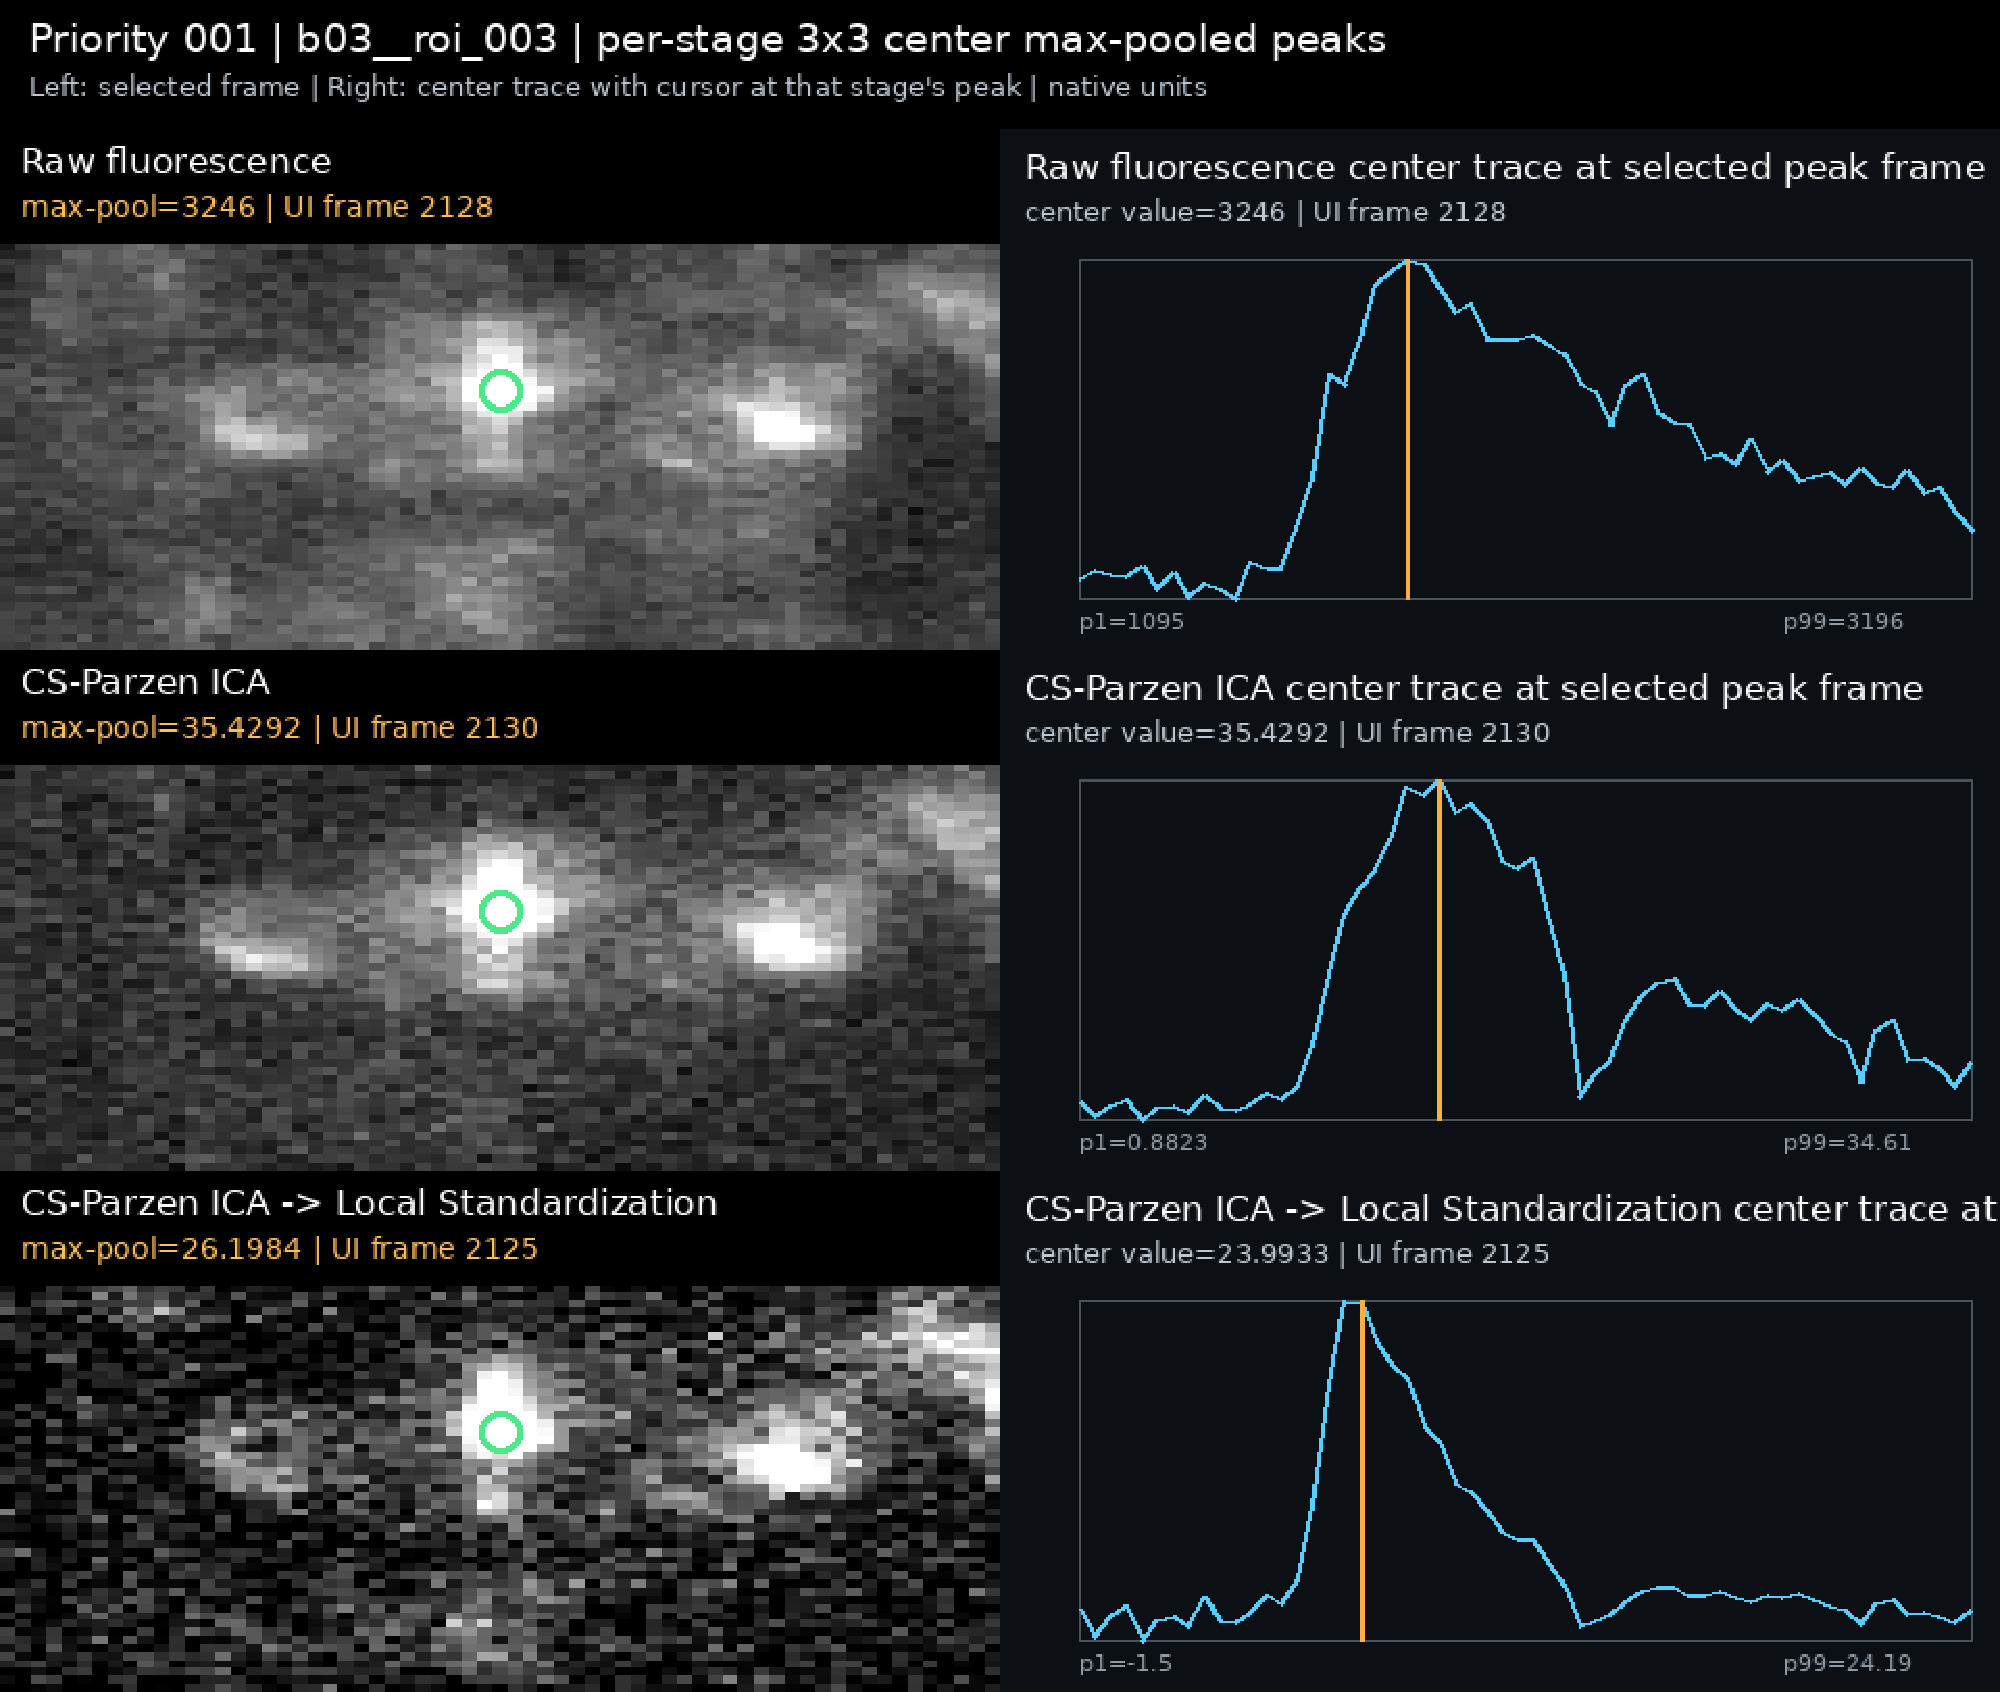
\includegraphics[page=1,width=0.98\linewidth]{figures/final/fig03_trace_atlas_examples.pdf}
  \caption{Frozen representative trace-atlas cases. (a) Hero: ROI~003 in burst~3, the frozen high-observability confirmed site. Left panels show each representation at its own $3\times3$ center max-pooled frame; right panels show the exact center trace with the selected frame marked. Values remain in representation-native units.}
  \label{fig:trace-atlas-cases}
\end{figure}

\begin{figure}[p]\ContinuedFloat
  \centering
  \includegraphics[page=2,width=0.98\linewidth]{figures/final/fig03_trace_atlas_examples.pdf}
  \caption{Frozen representative trace-atlas cases (continued). (b) Antihero: ROI~011 in burst~4, a confirmed but difficult observation site. ``Antihero'' denotes a hard known-positive case, not a negative or artifact.}
\end{figure}

\begin{figure}[p]\ContinuedFloat
  \centering
  \includegraphics[page=3,width=0.98\linewidth]{figures/final/fig03_trace_atlas_examples.pdf}
  \caption{Frozen representative trace-atlas cases (continued). (c) Random inclusion: ROI~010 in burst~3, selected from eligible confirmed four-burst sites with seed 20260824 before inspection of these panels. The original ROI~010 observation-site geometry is retained despite its provisional canonical merge with ROI~015.}
\end{figure}

\subsection{Trace reassessment supports two measurement profiles with incomplete stage preservation}

The reassessment in \Cref{fig:population-trace-summary} assigns all 50
coordinate-defined sites, representing 106 confirmed occurrences, from their
joint Raw, CS--Parzen ICA, and local-standardization trace shapes. The selected
two-class solution contained 38 and 12 sites. It had silhouette 0.261 and
median 80\% subsample adjusted Rand agreement 0.884, although the 10th
percentile agreement was 0.331. A three-class solution was admissible but had
lower silhouette (0.153) and median stability (0.727). Thus, two classes are
the preferred compact description, but the lower stability tail argues
against treating every site label as definitive.

Both classes show an onset-associated response. Trace Class~T1 has a more sustained
positive tail and higher native event peaks, whereas Trace Class~T2 returns toward or
below baseline more rapidly and has lower native peaks across the processed
representations. Amplitude was not used to fit these primary labels. Retaining
20 principal components reproduced the primary assignment exactly, and 12
components produced ARI 0.915; an eight-component compression was less stable
(ARI 0.358). Adding log native amplitude also changed assignments as its block
weight increased, confirming that shape and observability should remain
separate views rather than being collapsed into one nominal class.

\begin{figure}[p]
  \centering
  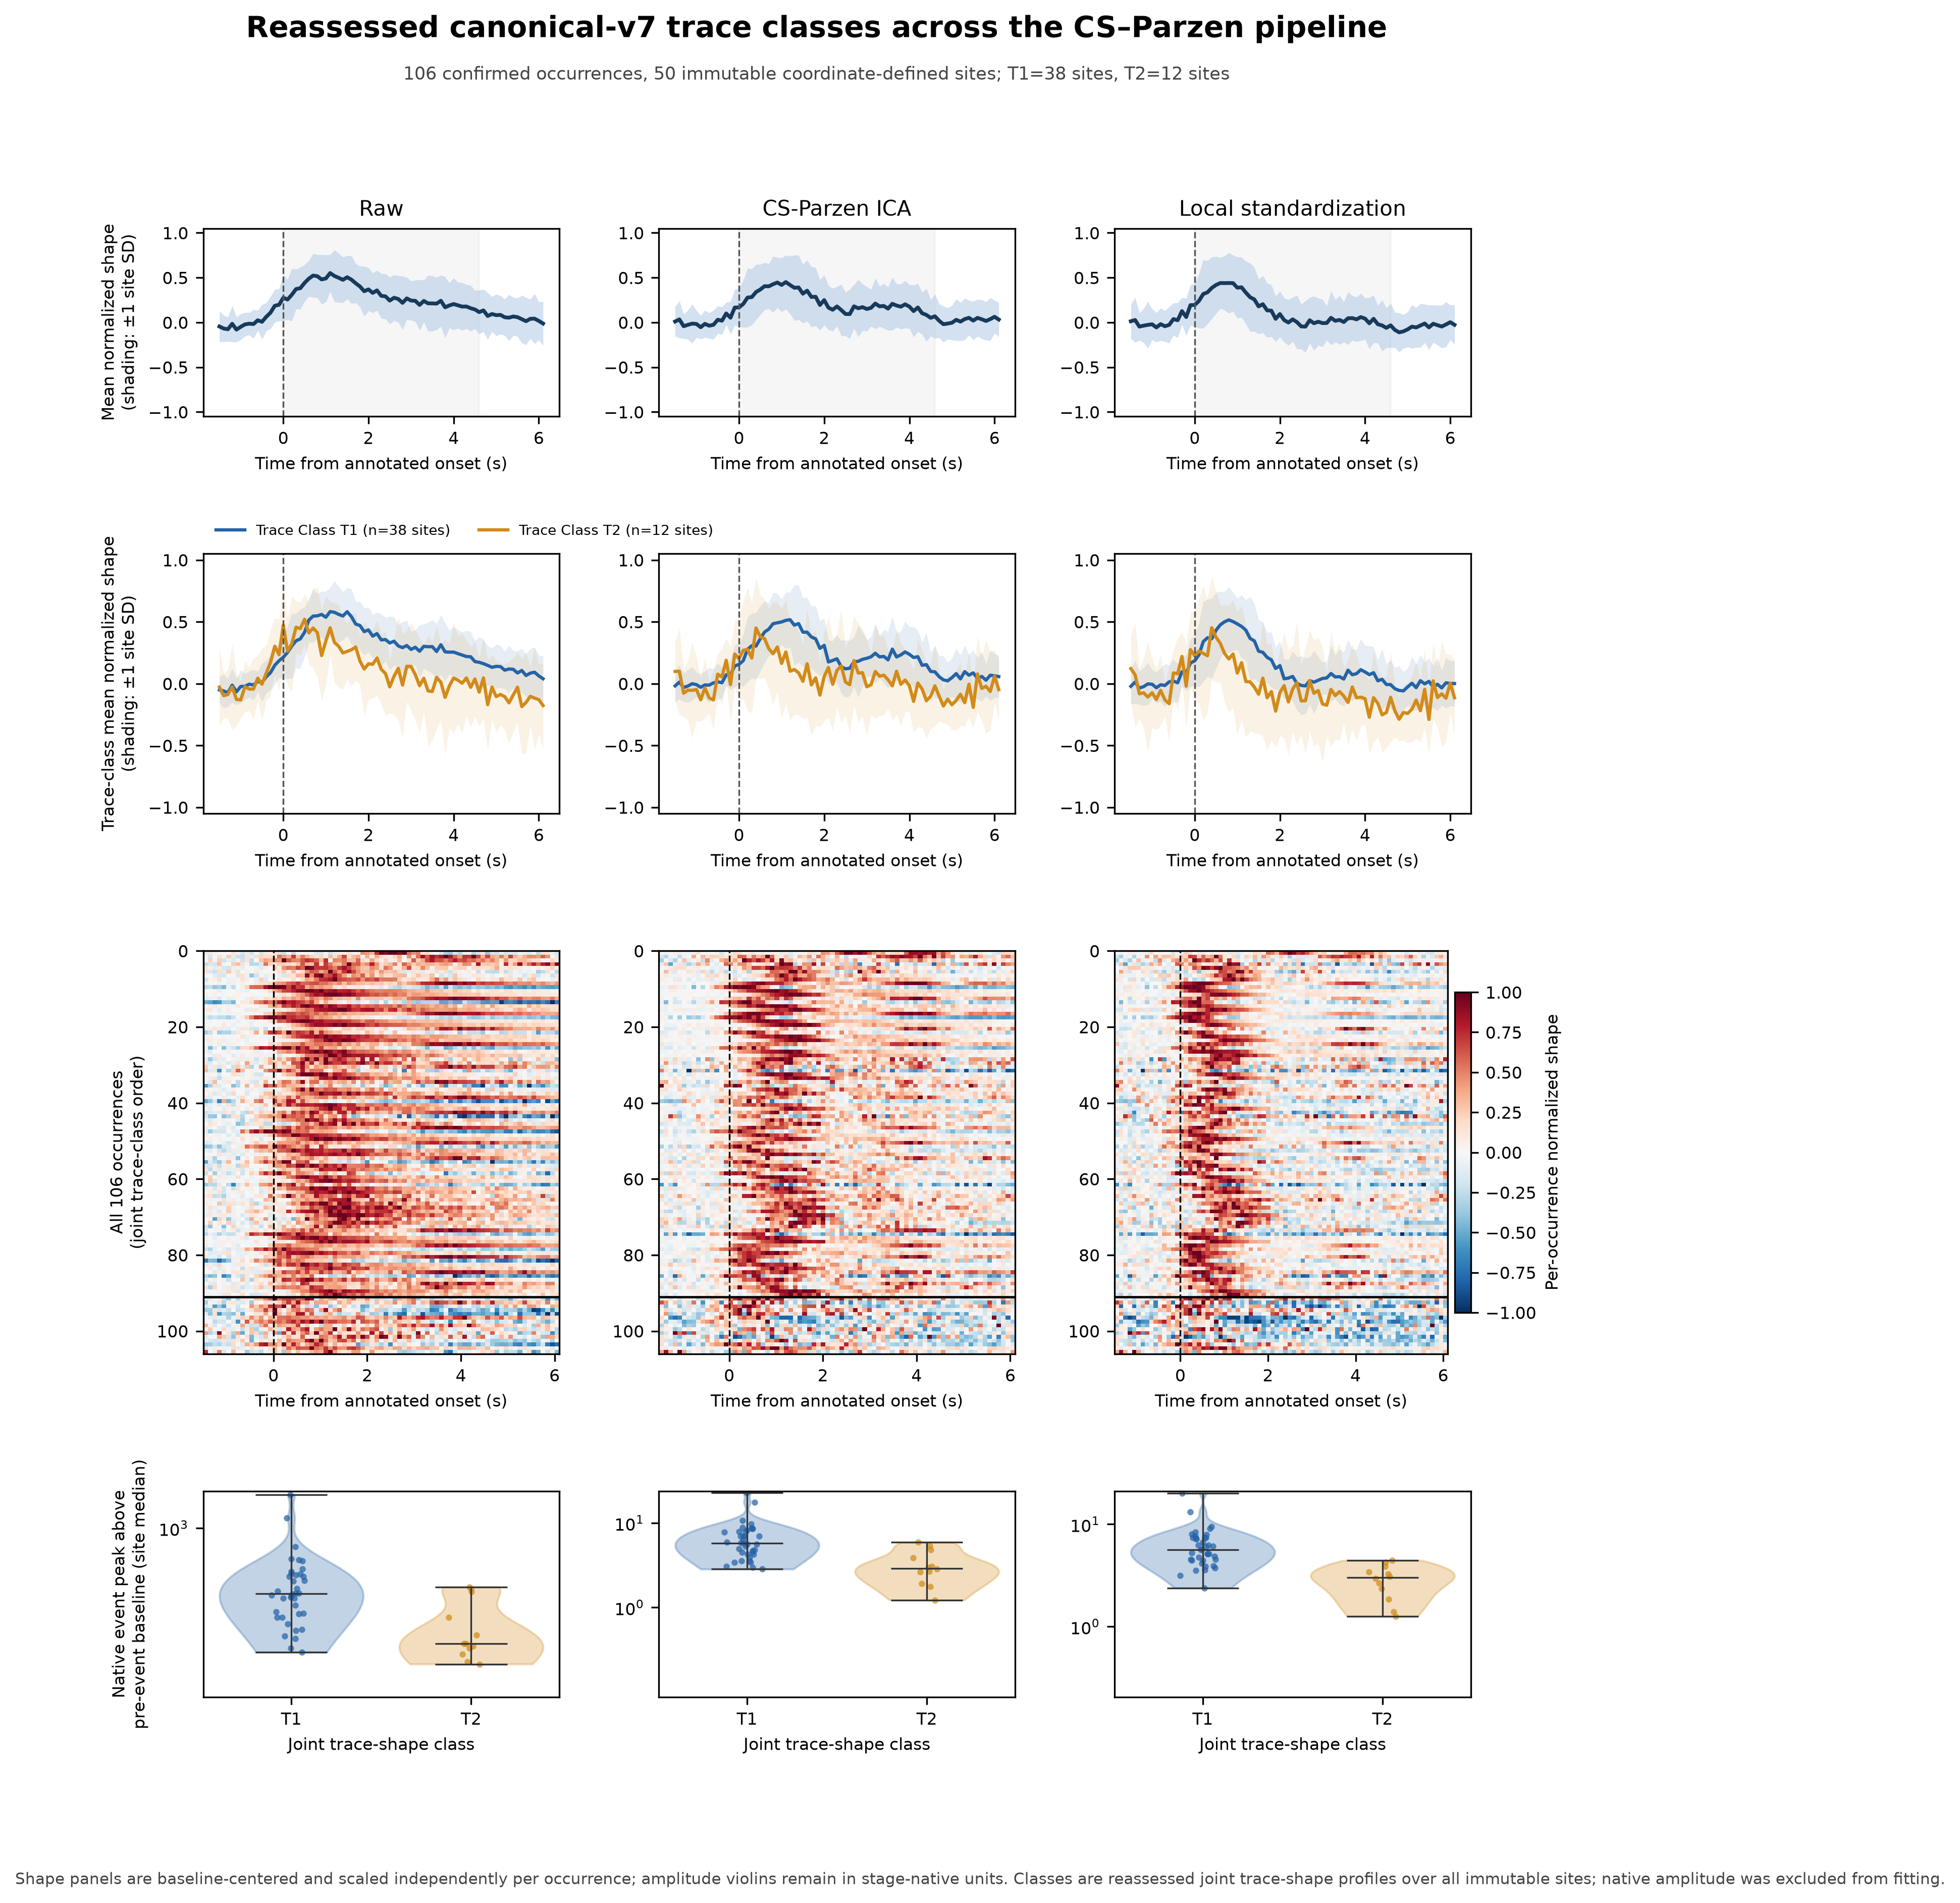
\includegraphics[width=0.98\linewidth]{figures/final/fig04_population_trace_summary.png}
  \caption{Reassessed population trace summary across Raw, CS--Parzen ICA, and local
  standardization. Top row: site-level mean normalized shape with $\pm1$
  site standard deviation. Second row: means and standard deviations for the
  two joint trace-shape classes. Third row: all confirmed occurrences in one
  fixed site/class order across representations; the heavy separator marks the
  class boundary. Bottom row: site-median native event-peak distributions,
  shown in representation-specific units. Traces
  are onset-aligned but not peak-aligned. Shape normalization is performed
  independently per occurrence and representation; the amplitude panels are
  not normalized across representations and amplitude was excluded from class
  fitting.}
  \label{fig:population-trace-summary}
\end{figure}

Independent stage fits did not preserve the smaller profile uniformly
(\Cref{fig:trace-taxonomy-stage-agreement}). Relative to the joint taxonomy,
Raw-only labels had ARI 0.578, CS--Parzen ICA-only labels 0.332, and
local-standardization-only labels 0.414. Every joint Trace Class~T1 site remained in
aligned stage Trace Class~T1, but only seven, four, and five of the 12 joint Trace Class~T2
sites were recovered by Raw, ICA, and local standardization, respectively.
Thirty-nine of 50 sites received the same aligned label in all three
stage-specific fits. This asymmetry suggests that the smaller joint profile is
defined partly by cross-stage information rather than by a stage-invariant
partition; it does not establish that the pipeline changes biological cell
identity.

\begin{figure}[!htbp]
  \centering
  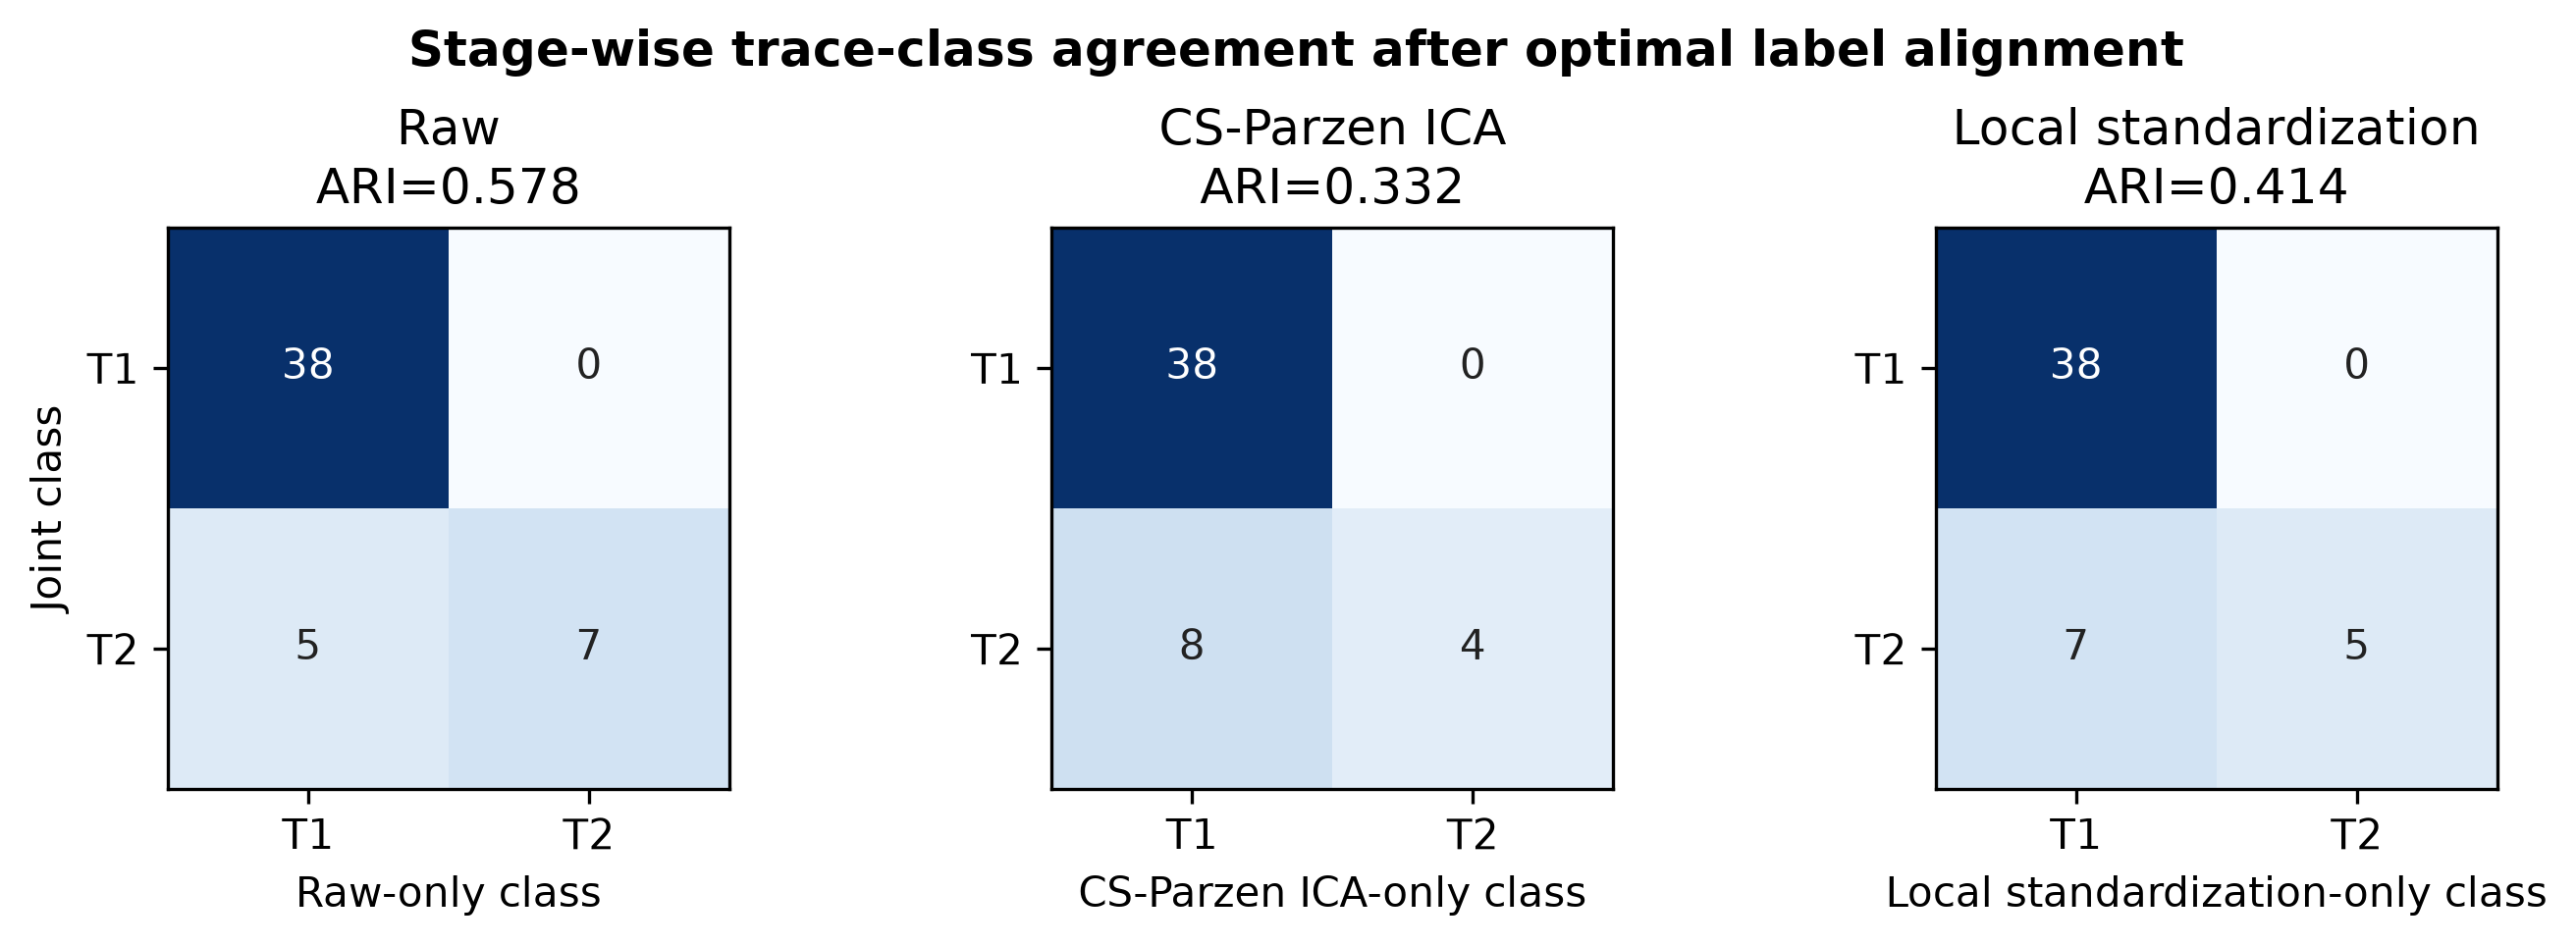
\includegraphics[width=0.98\linewidth]{figures/final/fig04b_trace_taxonomy_stage_agreement.png}
  \caption{Agreement between the joint two-class trace taxonomy and independent
  Raw-, CS--Parzen ICA-, and local-standardization-only fits. Labels were
  optimally permuted for display; adjusted Rand indices are permutation
  invariant. Counts are immutable coordinate-defined sites.}
  \label{fig:trace-taxonomy-stage-agreement}
\end{figure}

Leave-one-burst-out analysis favored a burst-dependent trace state over an
immutable site type (\Cref{fig:trace-taxonomy-lobo}). Eighty-one held-out
assignments from 25 recurrent sites were eligible. Site-blocked agreement with
the class learned from the other bursts was 0.740 (95\% bootstrap interval
0.647--0.833) and increased to 0.840 (0.740--0.927) when burst~2 was excluded.
Agreement by held-out burst was 0.824, 0.368, 0.708, and 1.000 for bursts
1--4, respectively. Only nine of 25 recurrent sites agreed with their
training-derived class in every available fold, and only three retained one
held-out label across all available bursts. The median centroid margin was
0.133, with 39.5\% of assignments below 0.10. Consequently, T1/T2 is retained
as a compact descriptive trace axis, but the evidence does not support two
immutable neuron classes. Burst state and boundary uncertainty are substantial,
with burst~2 the clearest source of instability.

\begin{figure}[p]
  \centering
  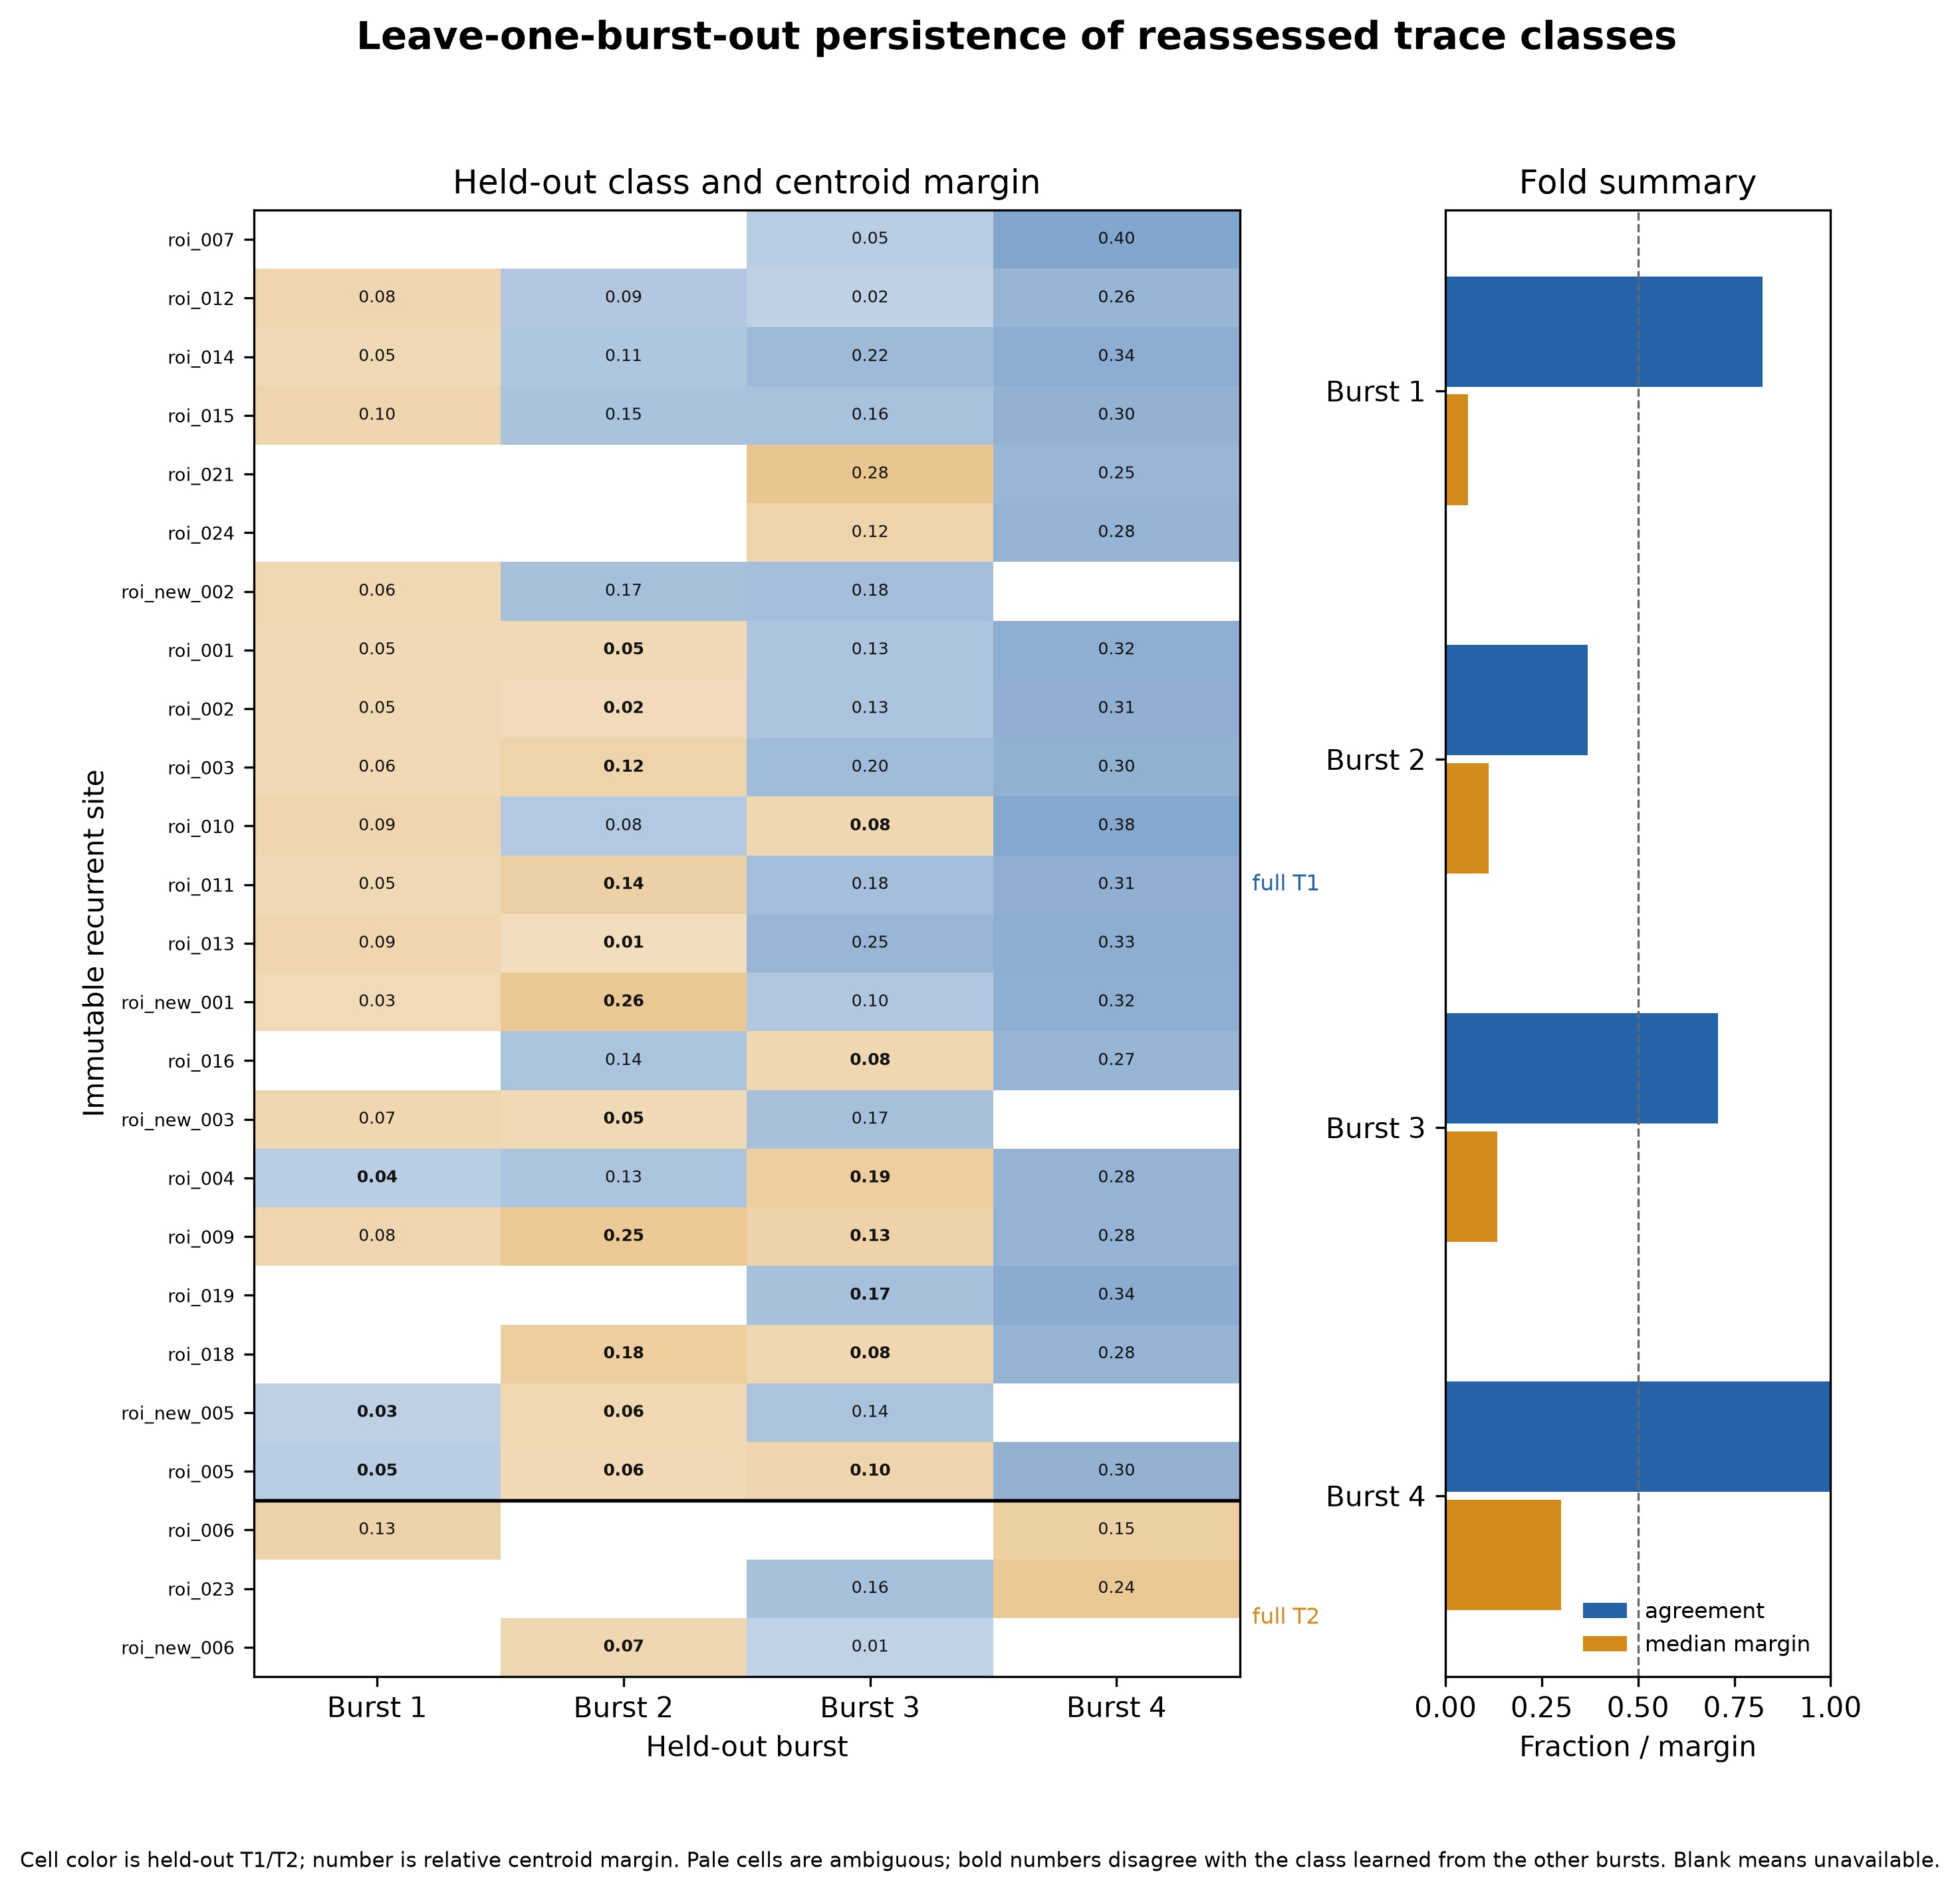
\includegraphics[width=0.98\linewidth]{figures/final/fig04c_trace_taxonomy_lobo_persistence.png}
  \caption{Leave-one-burst-out trace-class persistence for recurrent immutable
  sites. Cell color gives the held-out T1/T2 assignment and the printed value
  is the relative centroid margin; paler cells are closer to the boundary.
  Bold values disagree with the class learned from the other bursts. Blank
  cells indicate that the site was unavailable in that held-out burst. The
  side panel reports fold-level agreement and median margin.}
  \label{fig:trace-taxonomy-lobo}
\end{figure}

\subsection{The diagnostic audit separates transformation effects from missing model internals}

The audit contains 318 unique occurrence--stage rows (106 confirmed
occurrences by three representations) with no duplicate composite keys
(\Cref{fig:pipeline-diagnostic-audit}). Raw-to-ICA center traces had median
shape correlation 0.654 (10th--90th percentile 0.184--0.871) and median peak
shift $+0.2$~s. ICA-to-local-standardization traces were more similar (median
correlation 0.945, 10th--90th percentile 0.821--0.997) with median peak shift
zero. Median positive late-to-early persistence declined from 0.692 in Raw to
0.443 in ICA and 0.188 after local standardization. Thus the first transition
substantially changes waveform shape, whereas the second generally preserves
the immediate response while suppressing its late positive tail.

Burst~2 was also weak in native Raw measurements: its median peak was 283 and
median robust SNR 2.43, compared with peaks 352, 538, and 531 and SNRs 4.87,
8.79, and 10.08 in bursts 1, 3, and 4. This acquisition/event-strength
difference is consistent with, but does not by itself explain, the burst~2
class instability. Six of 106 local Raw crops contained at least one saturated
sample, but no labeled center trace reached the 4095 ceiling.

At the local-standardization stage, the binary T2 label was associated
descriptively with lower robust SNR ($\rho=-0.447$), lower center--annulus
contrast ($\rho=-0.353$), larger effective radius ($\rho=0.307$), and lower
center--annulus trace correlation ($\rho=-0.479$). Persistence itself had only
$\rho=0.188$ with the binary cut, reinforcing that the Ward partition is not a
threshold on one simple persistence statistic. These are post-fit descriptive
associations within one recording; trace-derived associations are not
independent validation.

The audit also identifies a more consequential information gap. Final Raw,
ICA, and local-standardization movies support temporal, neighborhood, and
spatial diagnostics, and candidate-match metadata cover 71 of 106 confirmed
occurrences. The saved output does not contain component activations or
contributions, mixing/unmixing matrices, learned filters, a compatible
reconstruction residual, the true local-standardization denominator, or a
motion field. At the time of the movie-only audit, component attribution and
denominator-failure explanations were therefore blocked.

\begin{figure}[p]
  \centering
  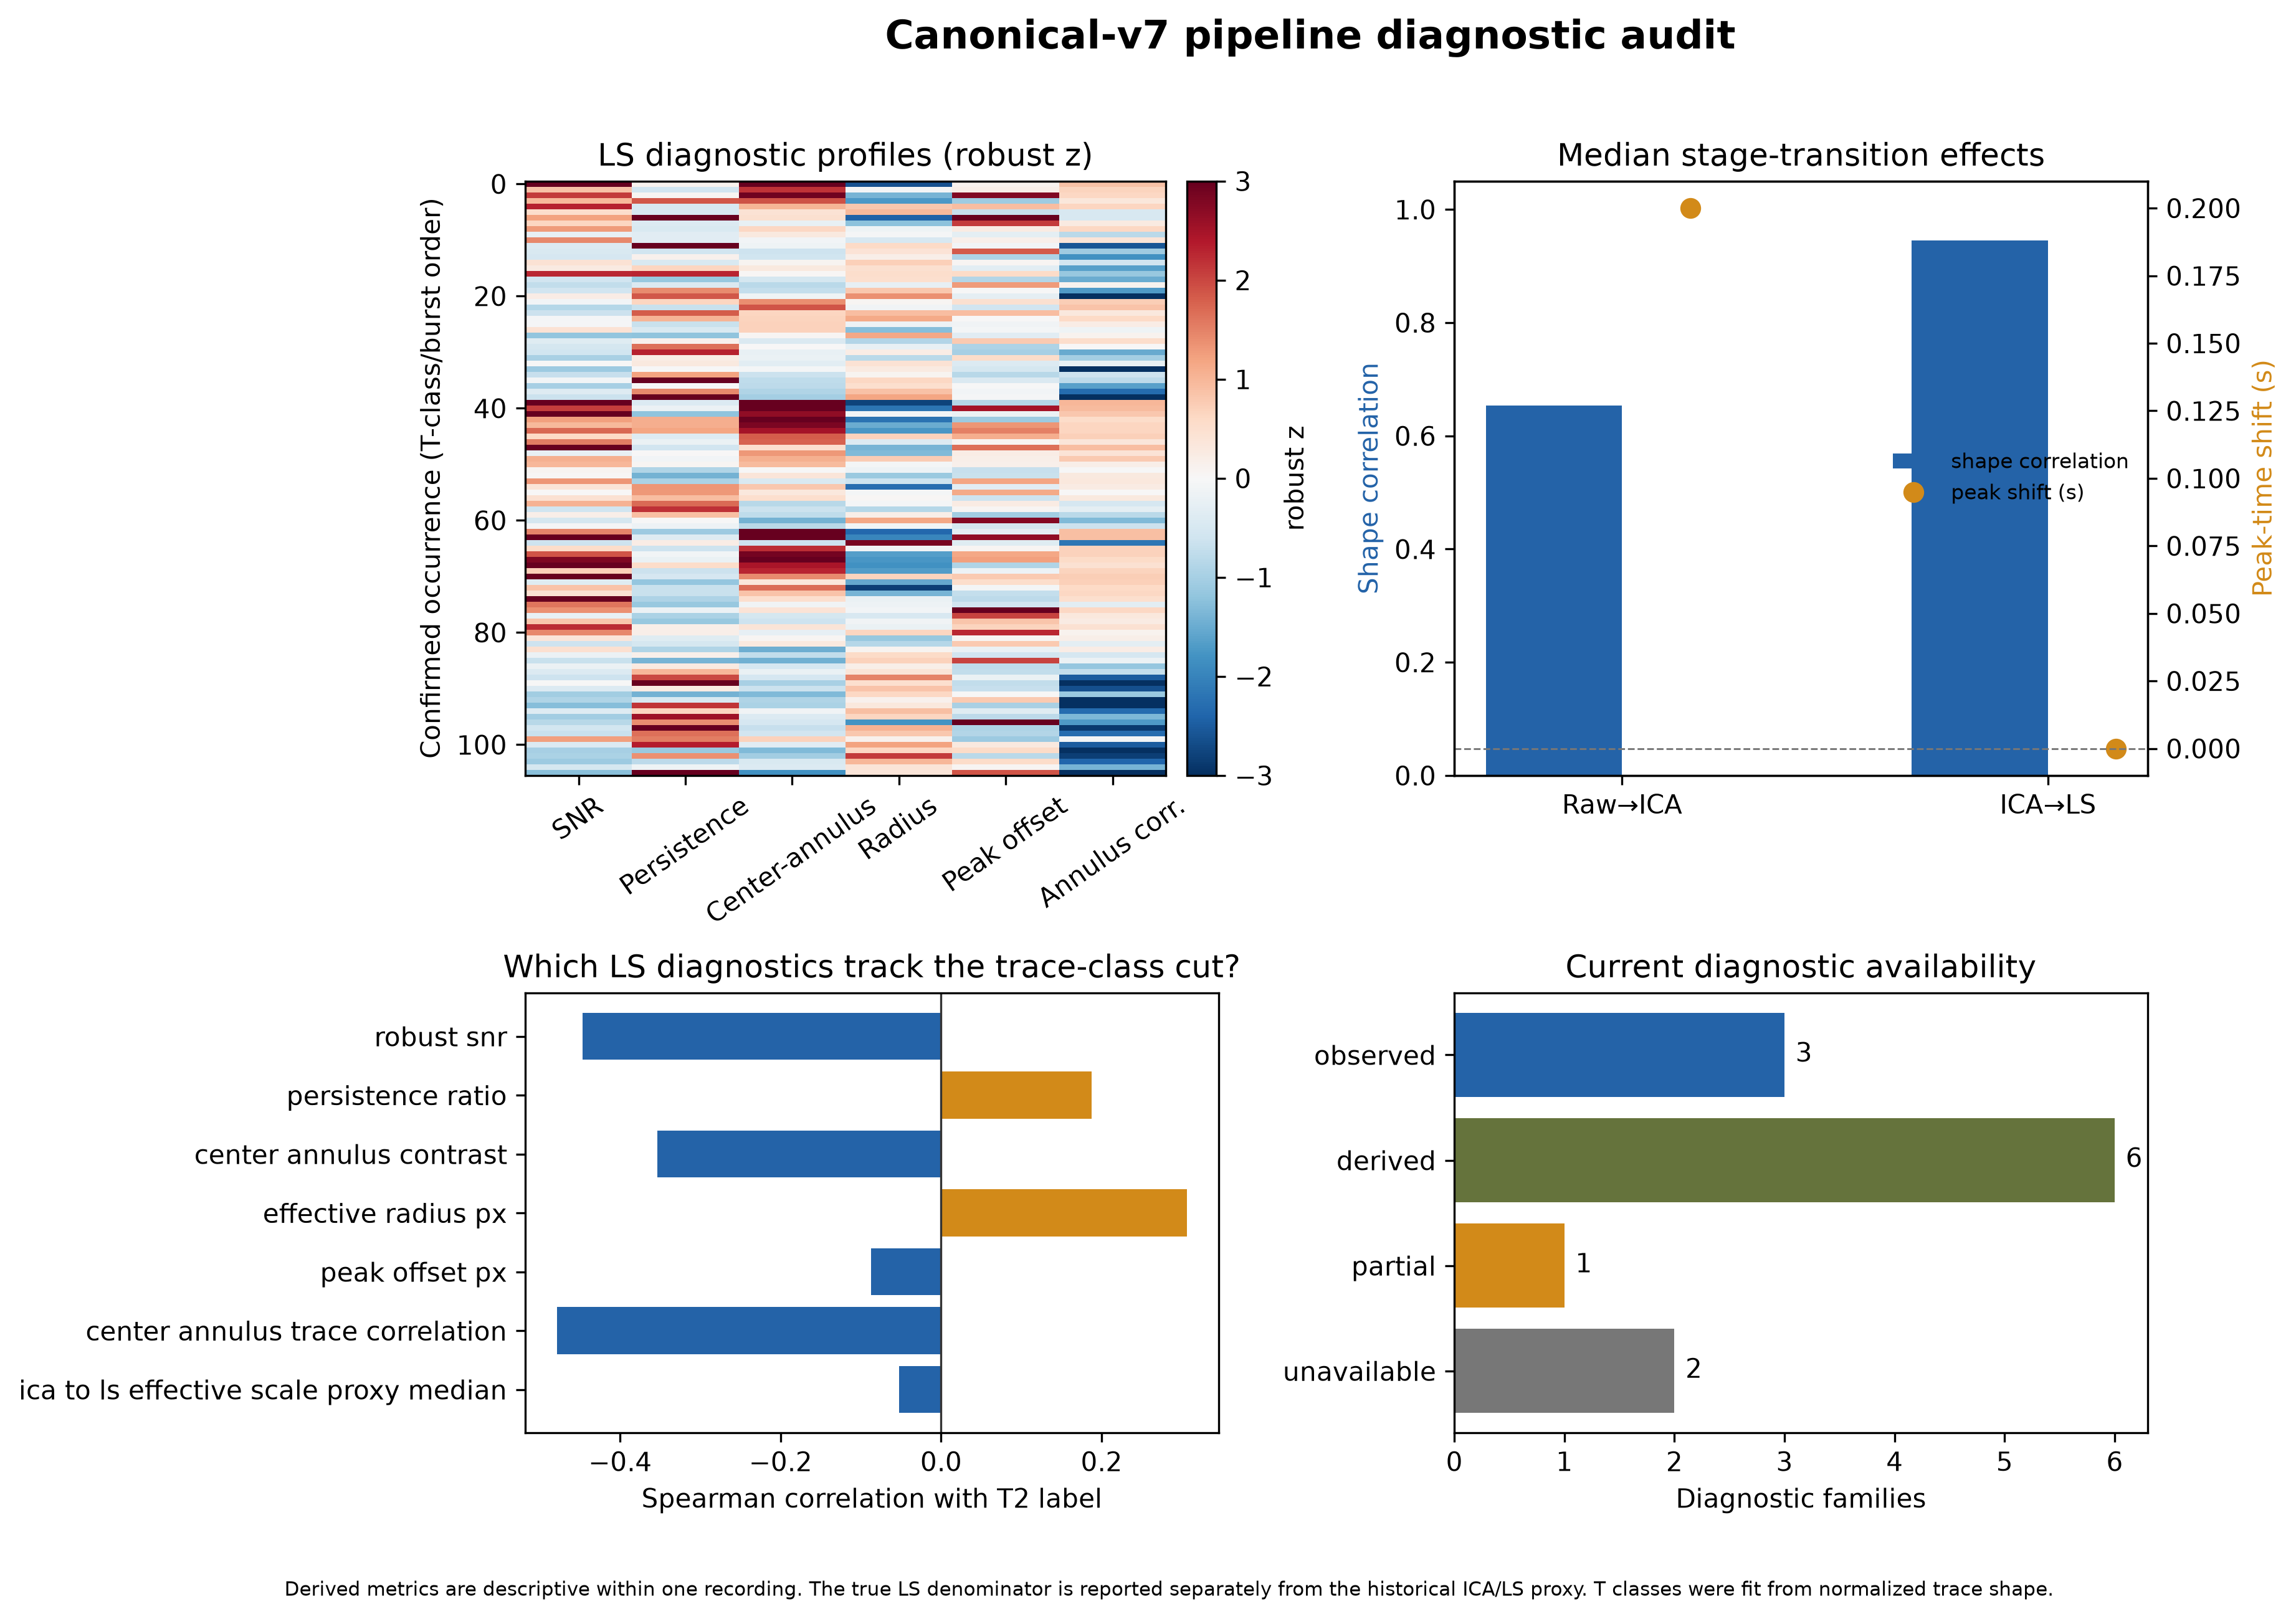
\includegraphics[width=0.98\linewidth]{figures/final/fig05_pipeline_diagnostic_audit.png}
  \caption{Canonical-v7 pipeline diagnostic audit. The heatmap shows robustly
  standardized local-standardization diagnostics for every confirmed
  occurrence. Stage-transition summaries use separate axes for trace
  correlation and peak-time shift. Correlations with T2 are descriptive and
  partially reuse trace information involved in class construction. The
  availability panel distinguishes observed, derived, partial, and unavailable
  diagnostic families.}
  \label{fig:pipeline-diagnostic-audit}
\end{figure}

The first model-internals refresh resolves the temporal-ICA portion of this gap
(\Cref{fig:ica-model-internals}). The frozen long-delay fit contains six
components over lags 0, 1, 2, 4, 8, and 16 frames; component~1 is the designated
persistence component, component~0 is innovation, and components~2--5 form the
reported residual group. Across all 50 unique sites, the full component traces,
mixing/demixing matrices, and energy fractions are now retained. The maximum
sitewise RMS embedding inversion residual was $5.69\times10^{-12}$, confirming
numerical invertibility at floating-point precision. This is deliberately not
reported as evidence of signal recovery or denoising quality. The true
local-standardization denominator is assessed separately below.

\begin{figure}[p]
  \centering
  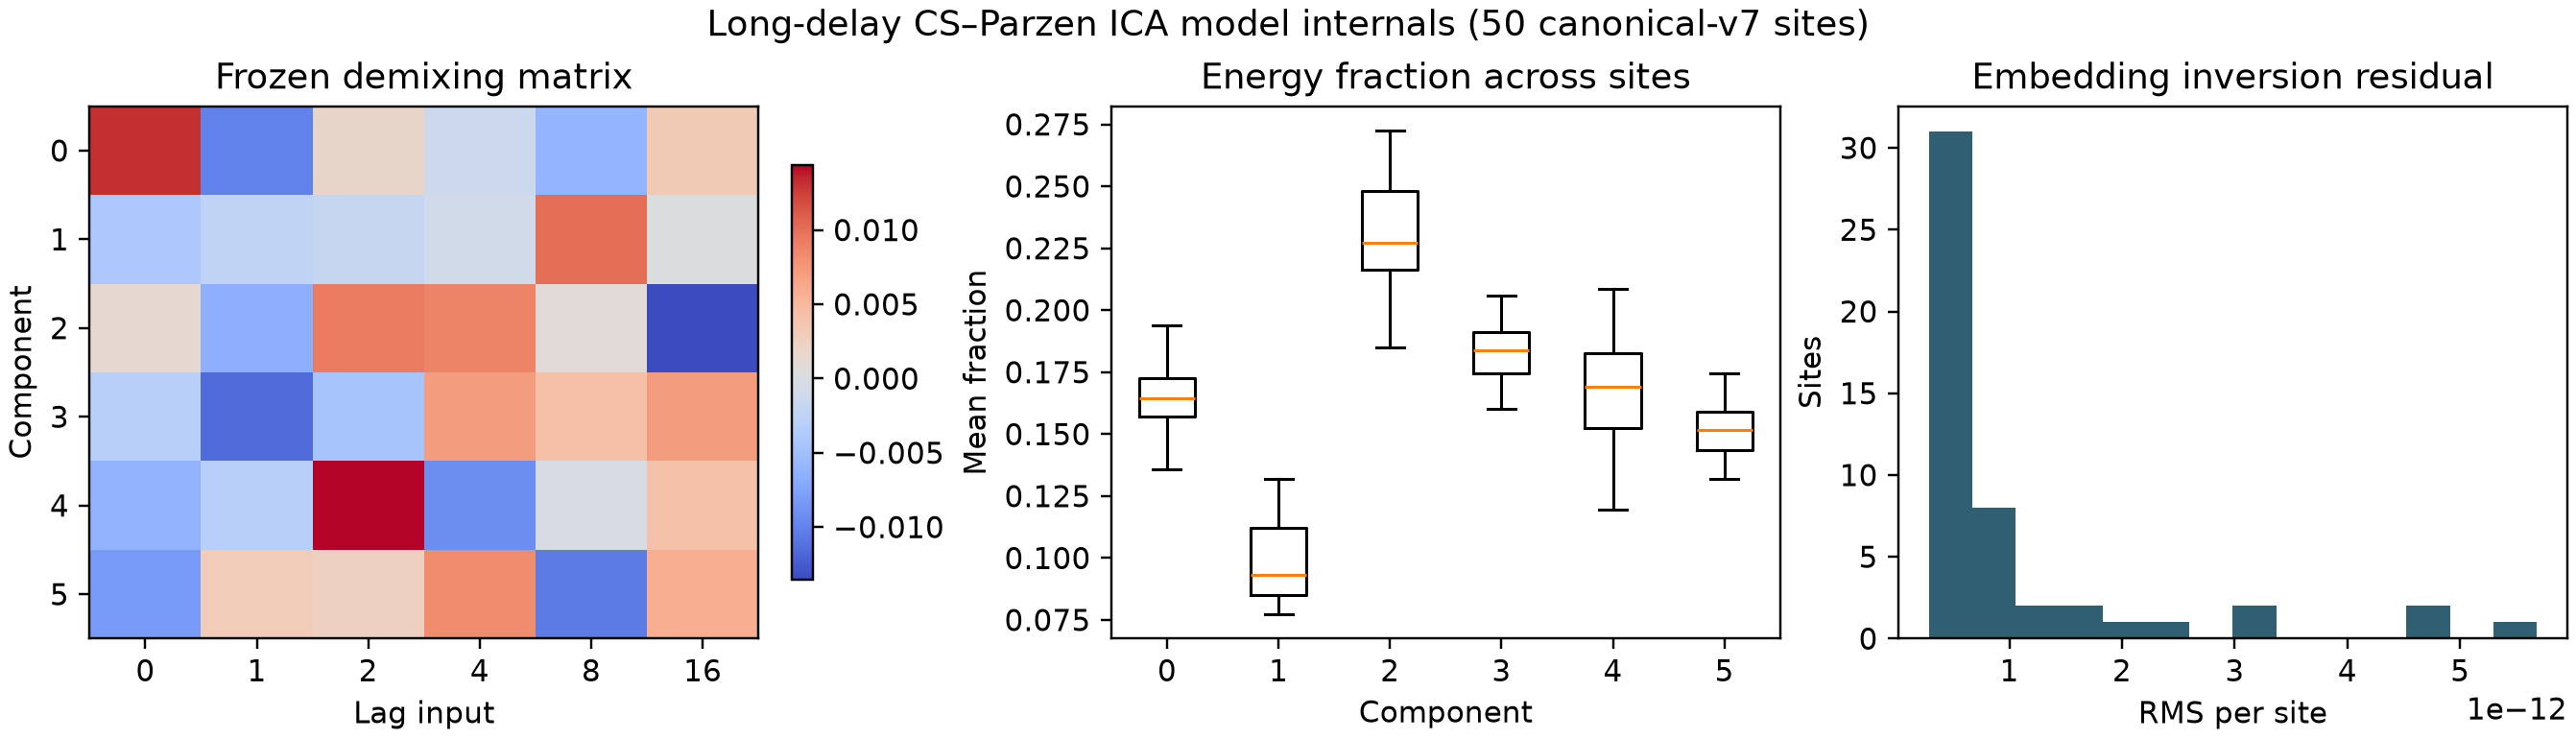
\includegraphics[width=0.98\linewidth]{figures/final/fig06_ica_model_internals.png}
  \caption{Frozen long-delay CS--Parzen ICA internals at the 50 unique
  canonical-v7 sites. Left, the learned demixing coefficients for lagged inputs.
  Middle, per-site temporal means of each component's squared-energy fraction.
  Right, numerical embedding inversion residuals. The right panel audits
  transform invertibility and is not a denoising-reconstruction metric.}
  \label{fig:ica-model-internals}
\end{figure}

The causal-pre-roll-preserving denominator audit reproduced the saved
local-standardization center traces with an overall RMS error of
$6.96\times10^{-7}$ and maximum absolute error of $7.63\times10^{-6}$
(\Cref{fig:ls-denominator-audit}). The frozen global scale floor was 0.371705,
whereas the median denominator across sites and frames was 0.7648. The floor
was not active at any of the 50 canonical-v7 centers during the 560-frame
review interval. Thus, center-trace amplification in this population is driven
by the measured local space--time scale rather than clipping to the global
floor. This does not rule out floor use elsewhere in the full field.

\begin{figure}[p]
  \centering
  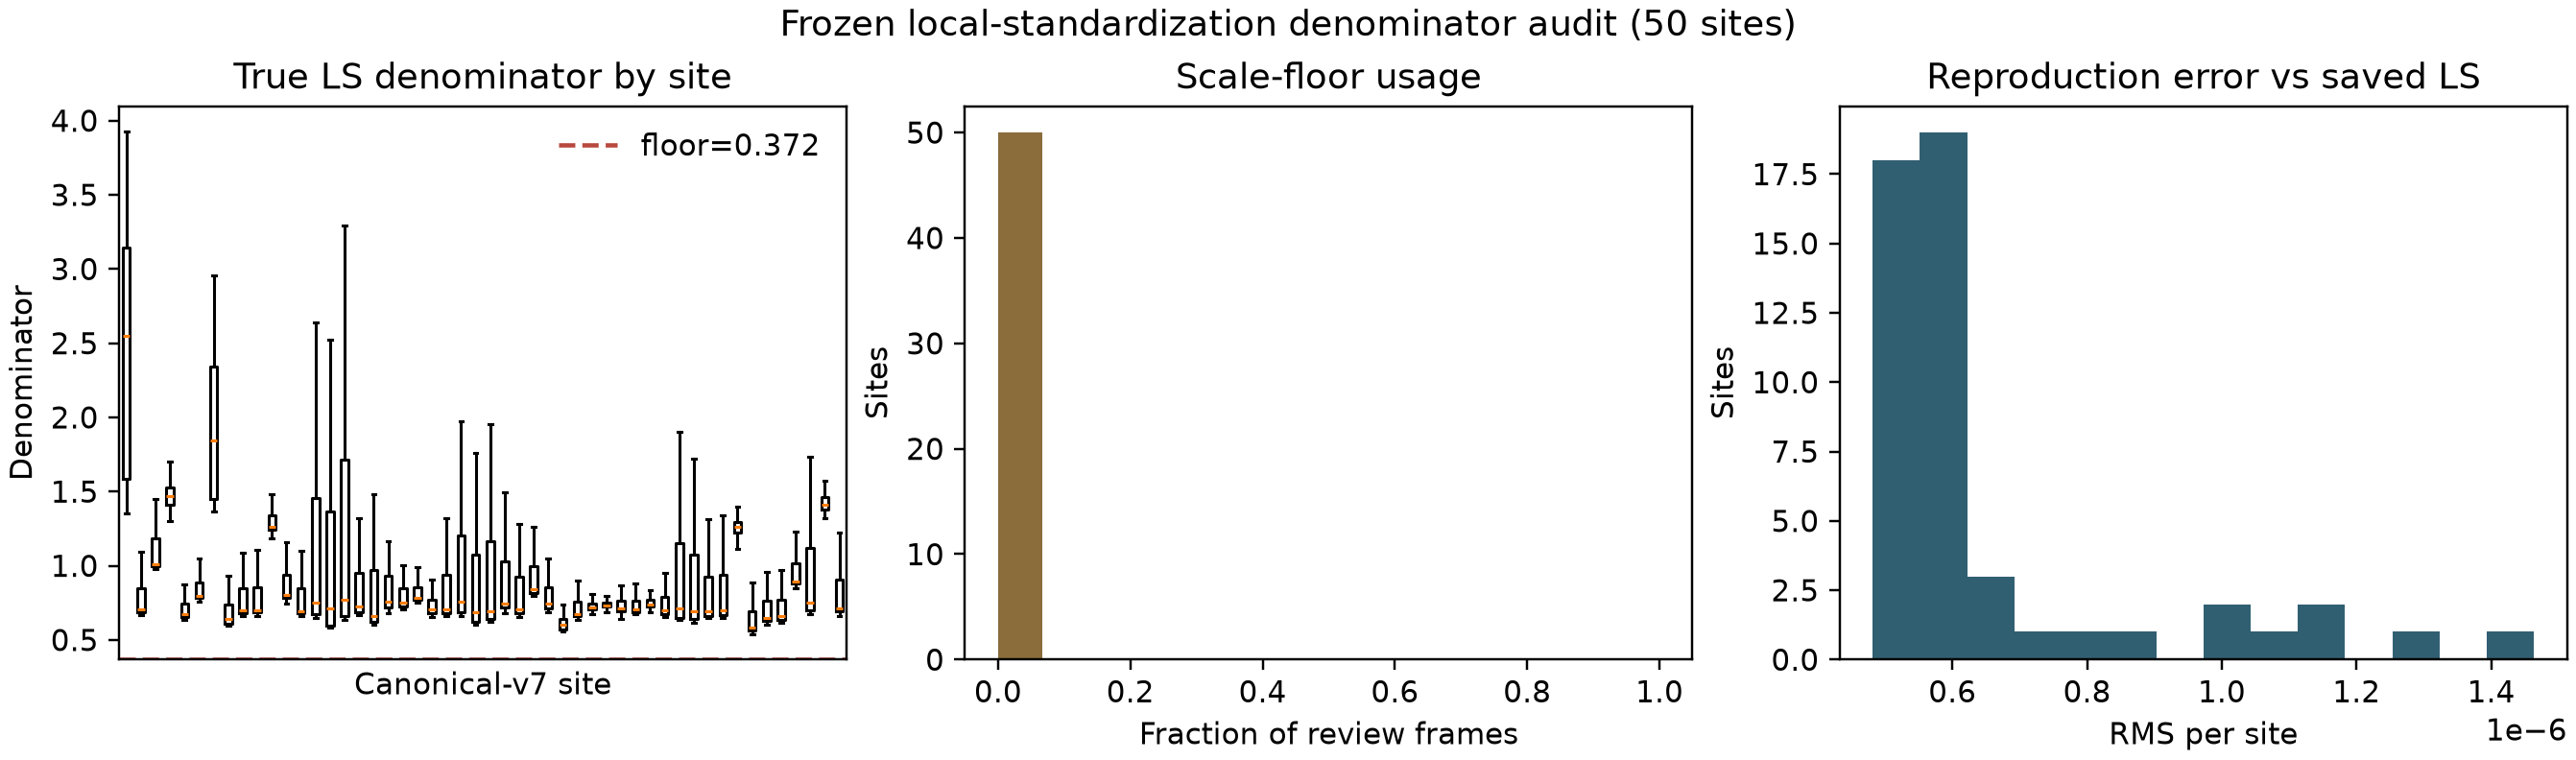
\includegraphics[width=0.98\linewidth]{figures/final/fig07_ls_denominator_diagnostics.png}
  \caption{Exact bounded reproduction of the frozen local-standardization
  denominator at 50 canonical-v7 sites. Left, denominator distributions by
  site with the saved global floor. Middle, the fraction of review frames for
  which the floor was active. Right, numerical agreement between reproduced
  and saved local-standardization center traces.}
  \label{fig:ls-denominator-audit}
\end{figure}

\subsection{Spatial/contextual features improve known-positive ranking without identifying precision}

In the earlier 79-observation full-field screen, carrier-only known-positive
recall at candidate budget 20 was \CarrierRecallBtwenty{}, compared with
\CoherenceRecallBtwenty{} for the cross-fitted local-coherence family and
\Provisional{0.5886} for the cross-fitted lagged-recurrence family. The exact
lag-2/15 lane reached the higher descriptive, post-hoc value
\LagRecallBtwenty{}. These values indicate that spatial and temporal context can
improve the ordering or proposal coverage of known positives. They do not
identify full-field precision because unmatched candidates may be unlabeled
neurons. The protected confirmation will hold proposals and non-maximum
suppression fixed where possible, separate proposal from ranking gains, and
reserve precision estimation for the exhaustively reviewed bounded field.

The complete-trace panel clarified why those contextual features should not be
treated as universal replacements for amplitude. At already confirmed centers,
the frozen carrier attained a site-weighted mean event-localization percentile
of \FullTraceCarrierPercentile{} (95\% site-bootstrap interval
\FullTraceCarrierCILow{}--\FullTraceCarrierCIHigh{}), while Raw, 15-frame
coherence, and lag-2 recurrence attained \FullTraceRawPercentile{},
\FullTraceCoherencePercentile{}, and \FullTraceLagPercentile{}, respectively.
The lagged score's paired difference from the carrier was only
\FullTraceLagDelta{} (95\% interval \FullTraceLagDeltaLow{}--
\FullTraceLagDeltaHigh{}) and did not pass the strictly positive interval gate.
The primary statistic was visibly ceiling-limited: \FullTraceCarrierCeilingCount{}/
\FullTraceOccurrences{} carrier scores, \FullTraceCoherenceCeilingCount{}/
\FullTraceOccurrences{} coherence scores, and \FullTraceLagCeilingCount{}/
\FullTraceOccurrences{} lag scores were exactly 1.0.

Neither prespecified extension improved localization over the carrier. The
Raw/ICA/local-standardization consensus reached
\FullTraceConsensusPercentile{}, and multiscale persistence reached
\FullTracePersistencePercentile{}. They did, however, retain cross-burst
site-rank variation after the strongest amplitude features saturated: median
available burst-pair Spearman correlations were
\FullTraceConsensusRepeatability{} and
\FullTracePersistenceRepeatability{}. Conversely, variance-stabilized
center-minus-annulus contrast reached \FullTraceVSTPercentile{}, supporting its
use as a noise/local-contamination diagnostic rather than the primary event
carrier. Thus the combined evidence assigns features to different roles:
amplitude for event strength at a known center, coherence for proposal and
early-budget ranking, recurrence as secondary temporal context, and
consensus/persistence as exploratory observability features.

\begin{table}[!htbp]
\centering
\scriptsize
\begin{tabularx}{\linewidth}{X r r r}
\toprule
Feature & Mean percentile [95\% CI] & $\Delta$ vs carrier & Median $\rho$ \\
\midrule
Raw center & 0.991 [0.973, 1.000] & -0.003 & -- \\
CS-Parzen ICA center & 0.964 [0.927, 0.992] & -0.030 & -- \\
Local standardization center & 0.935 [0.894, 0.969] & -0.059 & 0.524 \\
Raw center-annulus & 0.907 [0.857, 0.949] & -0.086 & 0.377 \\
VST center-annulus & 0.883 [0.824, 0.934] & -0.111 & 0.492 \\
LS exponential matched filter & 0.958 [0.918, 0.990] & -0.036 & -- \\
Frozen amplitude carrier & 0.994 [0.981, 1.000] & +0.000 & -- \\
Local coherence (15 frames) & 0.994 [0.981, 1.000] & +0.000 & -- \\
Lag-2 recurrence (15 frames) & 0.996 [0.987, 1.000] & +0.002 & -- \\
Raw/ICA/LS consensus & 0.986 [0.963, 0.999] & -0.008 & 0.633 \\
LS multiscale persistence & 0.972 [0.945, 0.992] & -0.022 & 0.649 \\
\bottomrule
\end{tabularx}
\caption{Exploratory full-trace feature panel at confirmed ROI centers. Percentiles compare each confirmed event maximum with all same-duration quiet-window maxima at the same immutable site; intervals use a 5,000-draw site bootstrap. The final column is the median available burst-pair Spearman correlation of site ranks; dashes denote ceiling-induced undefined correlations.}
\label{tab:full-trace-feature-panel}
\end{table}


\begin{figure}[p]
  \centering
  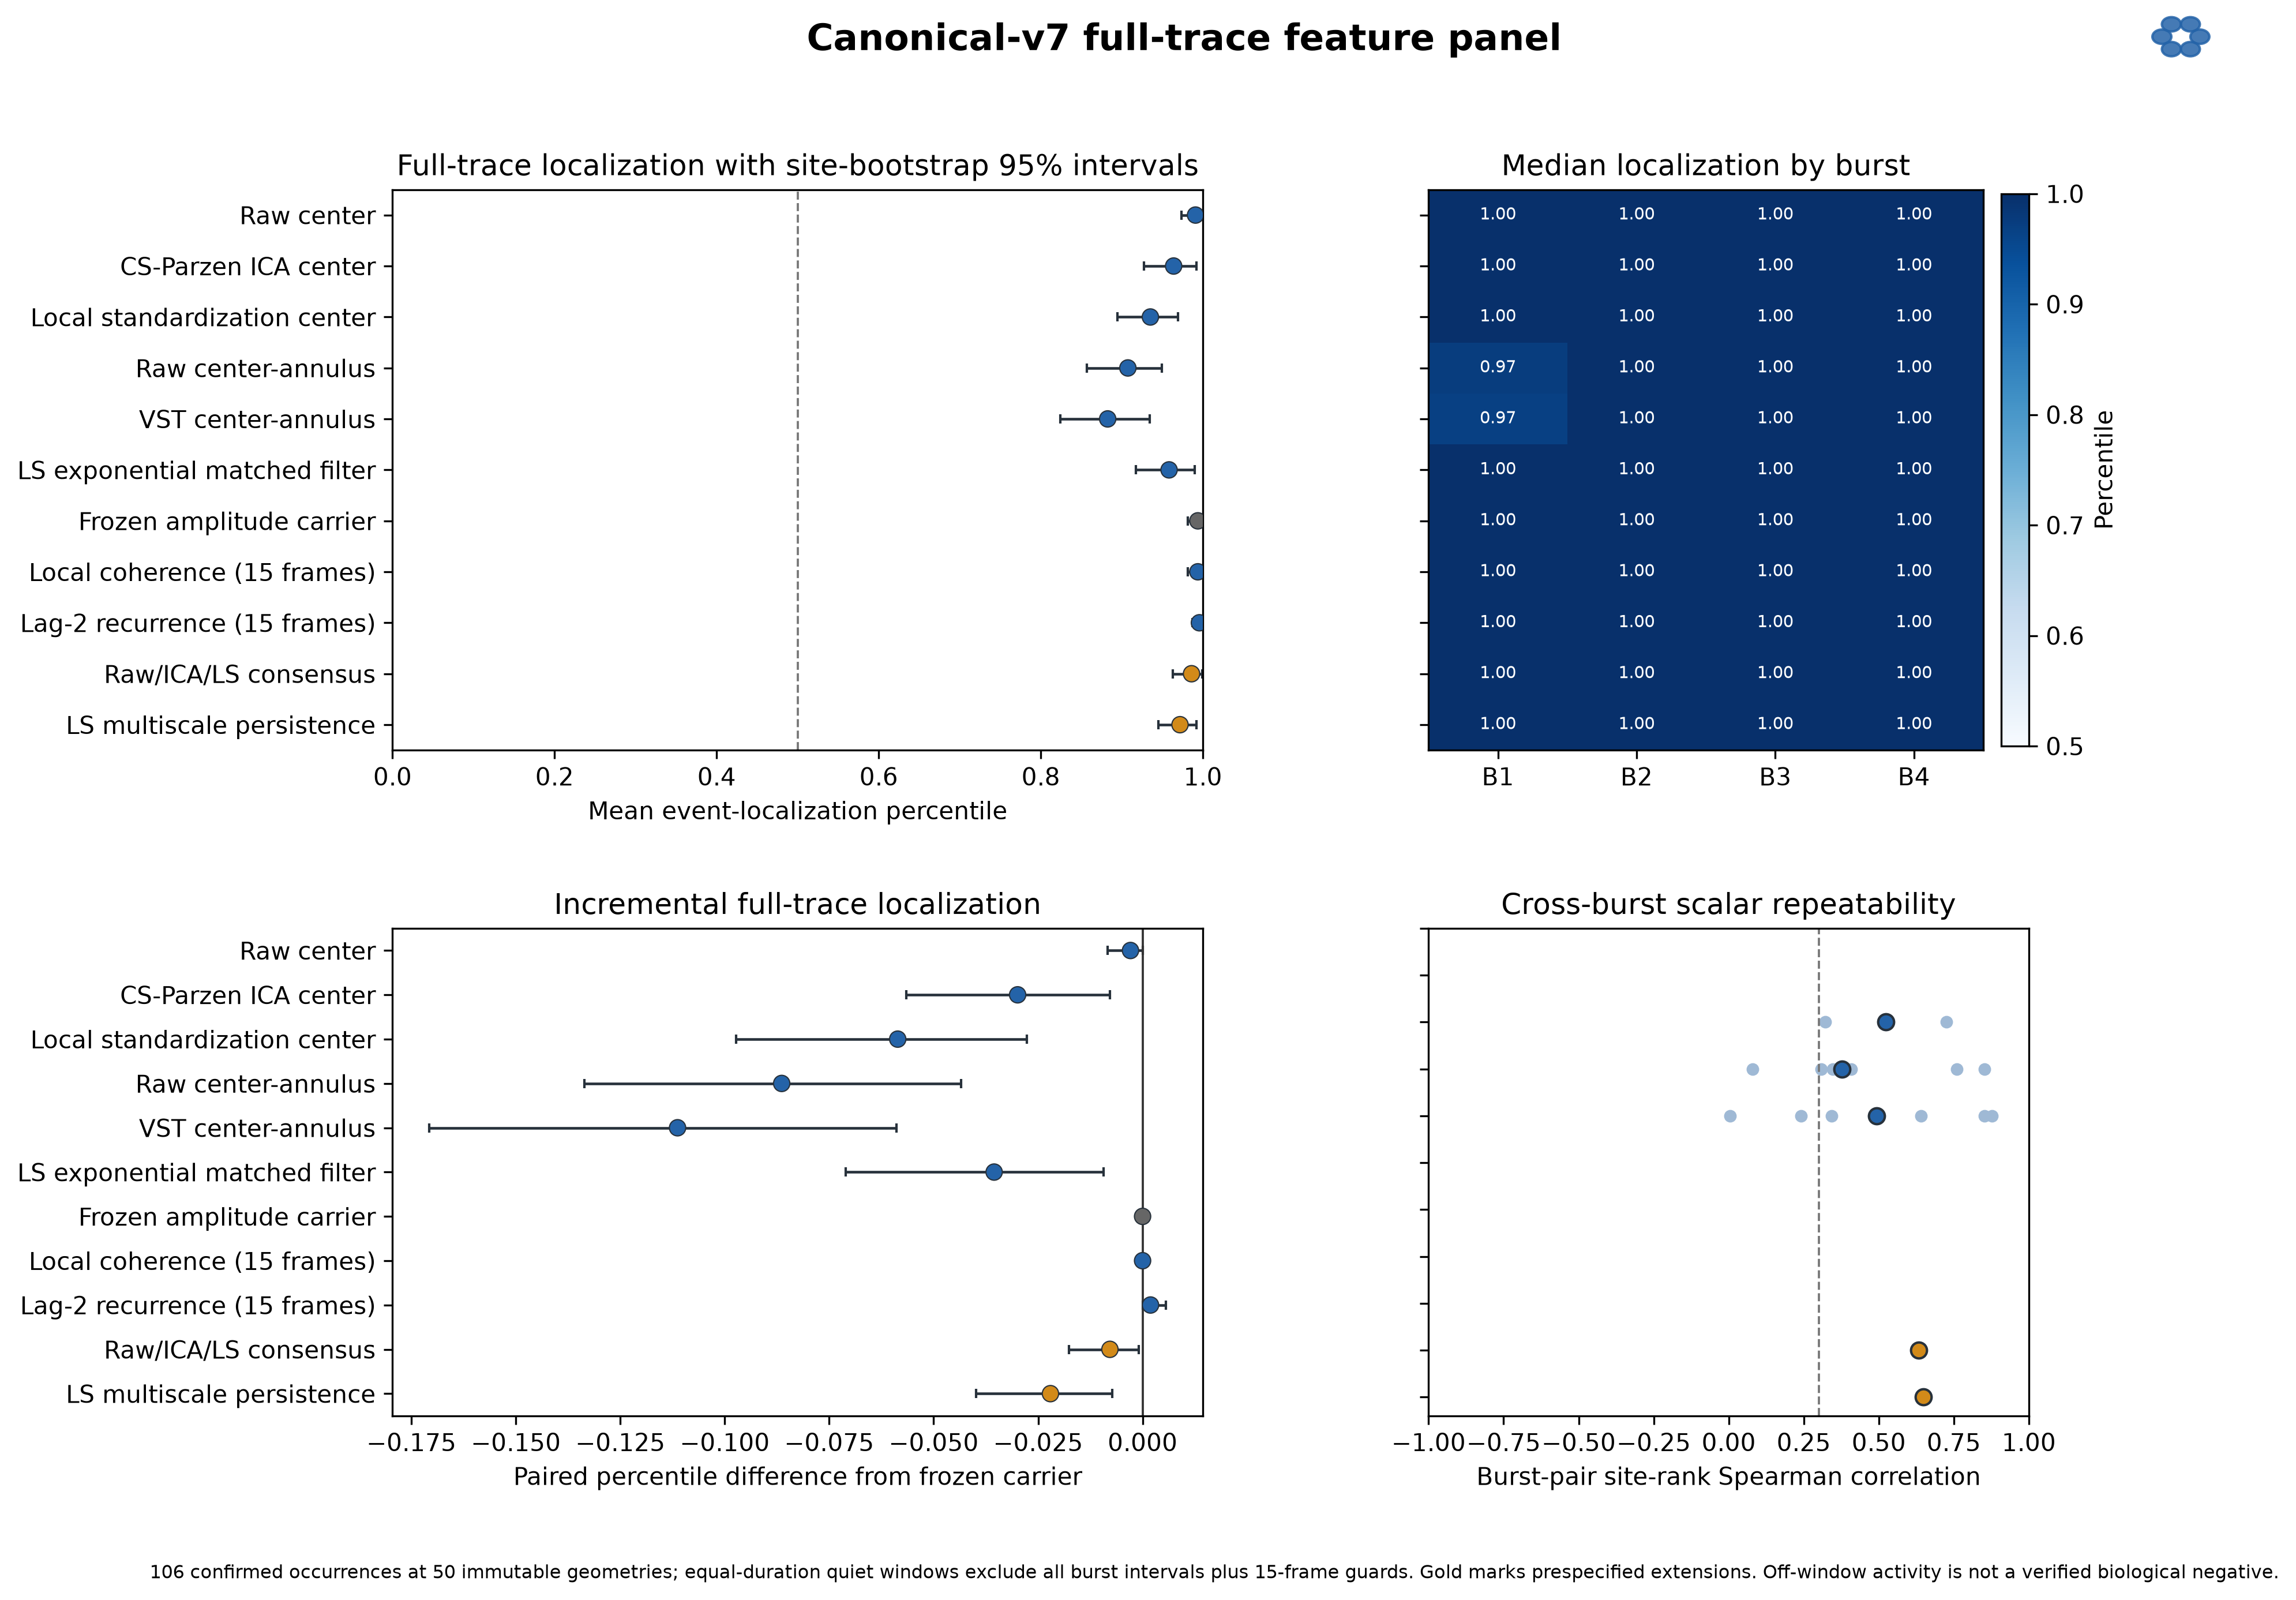
\includegraphics[width=0.98\linewidth]{figures/final/fig08_full_trace_feature_panel.png}
  \caption{Exploratory complete-trace feature panel for 106 confirmed
  occurrences at 50 immutable sites. Event maxima are compared with all
  same-duration guarded quiet-window maxima at the same site. Gold points are
  prespecified extensions. Undefined rank correlations arise when a burst is
  constant at the localization ceiling; quiet windows are not verified
  biological negatives.}
  \label{fig:full-trace-feature-panel}
\end{figure}

\subsection{Automated challenges support localized feature roles but not confirmed complementarity}

Replacing event maxima with frame-level event-versus-quiet retrieval removed
the earlier ceiling. Raw was strongest at \AutoRawAUC{} (95\% site-bootstrap
interval \AutoRawAUCLow{}--\AutoRawAUCHigh{}), followed by the carrier
(\AutoCarrierAUC{}), coherence (\AutoCoherenceAUC{}), lag-2 recurrence
(\AutoLagAUC{}), and the exponential matched filter (\AutoMatchedAUC{}).
All six compact spatial-challenge features had positive true-minus-displaced
AUC intervals. Multiscale persistence showed the largest paired difference,
\AutoPersistenceSpatialDelta{}, but its absolute temporal retrieval and
coordinate-jitter tolerance were lower than the amplitude/context lanes.

At budget 58, \AutoRecoveryCount{}/\FullTraceOccurrences{} original geometries
were recovered by at least one quantitative lane and \AutoRecoveryMisses{} were
missed. The carrier-only site-grouped model had cross-fitted log loss
\AutoCarrierLogLoss{} and ROC AUC 0.605; the role-specific model reached log
loss \AutoExtendedLogLoss{} and ROC AUC 0.826. The log-loss improvement was
\AutoRecoveryDelta{}, but its site-bootstrap interval was
\AutoRecoveryDeltaLow{}--\AutoRecoveryDeltaHigh{} and crossed zero. The
canonical-collapsed 102-row sensitivity was directionally similar, so the
feature panel is promising for error stratification but does not pass the
prespecified complementarity gate.

Reliability and event utility were not interchangeable. Raw center-annulus had
a site variance fraction of \AutoAnnulusReliability{} despite weak temporal
retrieval, whereas the carrier combined strong retrieval with a lower fraction
of \AutoCarrierReliability{}. All selected observed alignments exceeded 500
site-blocked circular shifts (minimum attainable upper-tail
$p=\AutoNullP{}$). Synthetic injections showed monotonic response; the matched
filter rose from mean AUC 0.531 at zero injection to 0.933 at four quiet-MAD
units, exceeding LS amplitude and persistence. These outcomes validate temporal
alignment and operator sensitivity, not neuron identity.

\begin{table}[!htbp]
\centering
\scriptsize
\begin{tabularx}{\linewidth}{X r r r}
\toprule
Feature & Frame AUC [95\% CI] & Spatial $\Delta$ AUC & Site fraction \\
\midrule
Raw center & 0.931 [0.906, 0.952] & 0.147 & 0.510 \\
Frozen amplitude carrier & 0.920 [0.896, 0.941] & 0.152 & 0.580 \\
Local coherence (15 frames) & 0.915 [0.890, 0.938] & 0.171 & 0.741 \\
Lag-2 recurrence (15 frames) & 0.905 [0.878, 0.927] & 0.169 & 0.735 \\
LS exponential matched filter & 0.884 [0.843, 0.917] & -- & 0.687 \\
Raw/ICA/LS consensus & 0.803 [0.776, 0.828] & 0.152 & 0.756 \\
LS multiscale persistence & 0.780 [0.742, 0.817] & 0.217 & 0.770 \\
Raw center-annulus & 0.727 [0.685, 0.773] & -- & 0.866 \\
\bottomrule
\end{tabularx}
\caption{Automated full-trace validation. Frame AUC separates annotated event frames from guarded quiet-reference frames. Spatial differences compare the true center with same-field baseline-matched displaced tissue. Site fraction is a nonparametric variance fraction, not REML ICC. Quiet and displaced references have unknown biological labels.}
\label{tab:automated-feature-validation}
\end{table}


\begin{figure}[p]
  \centering
  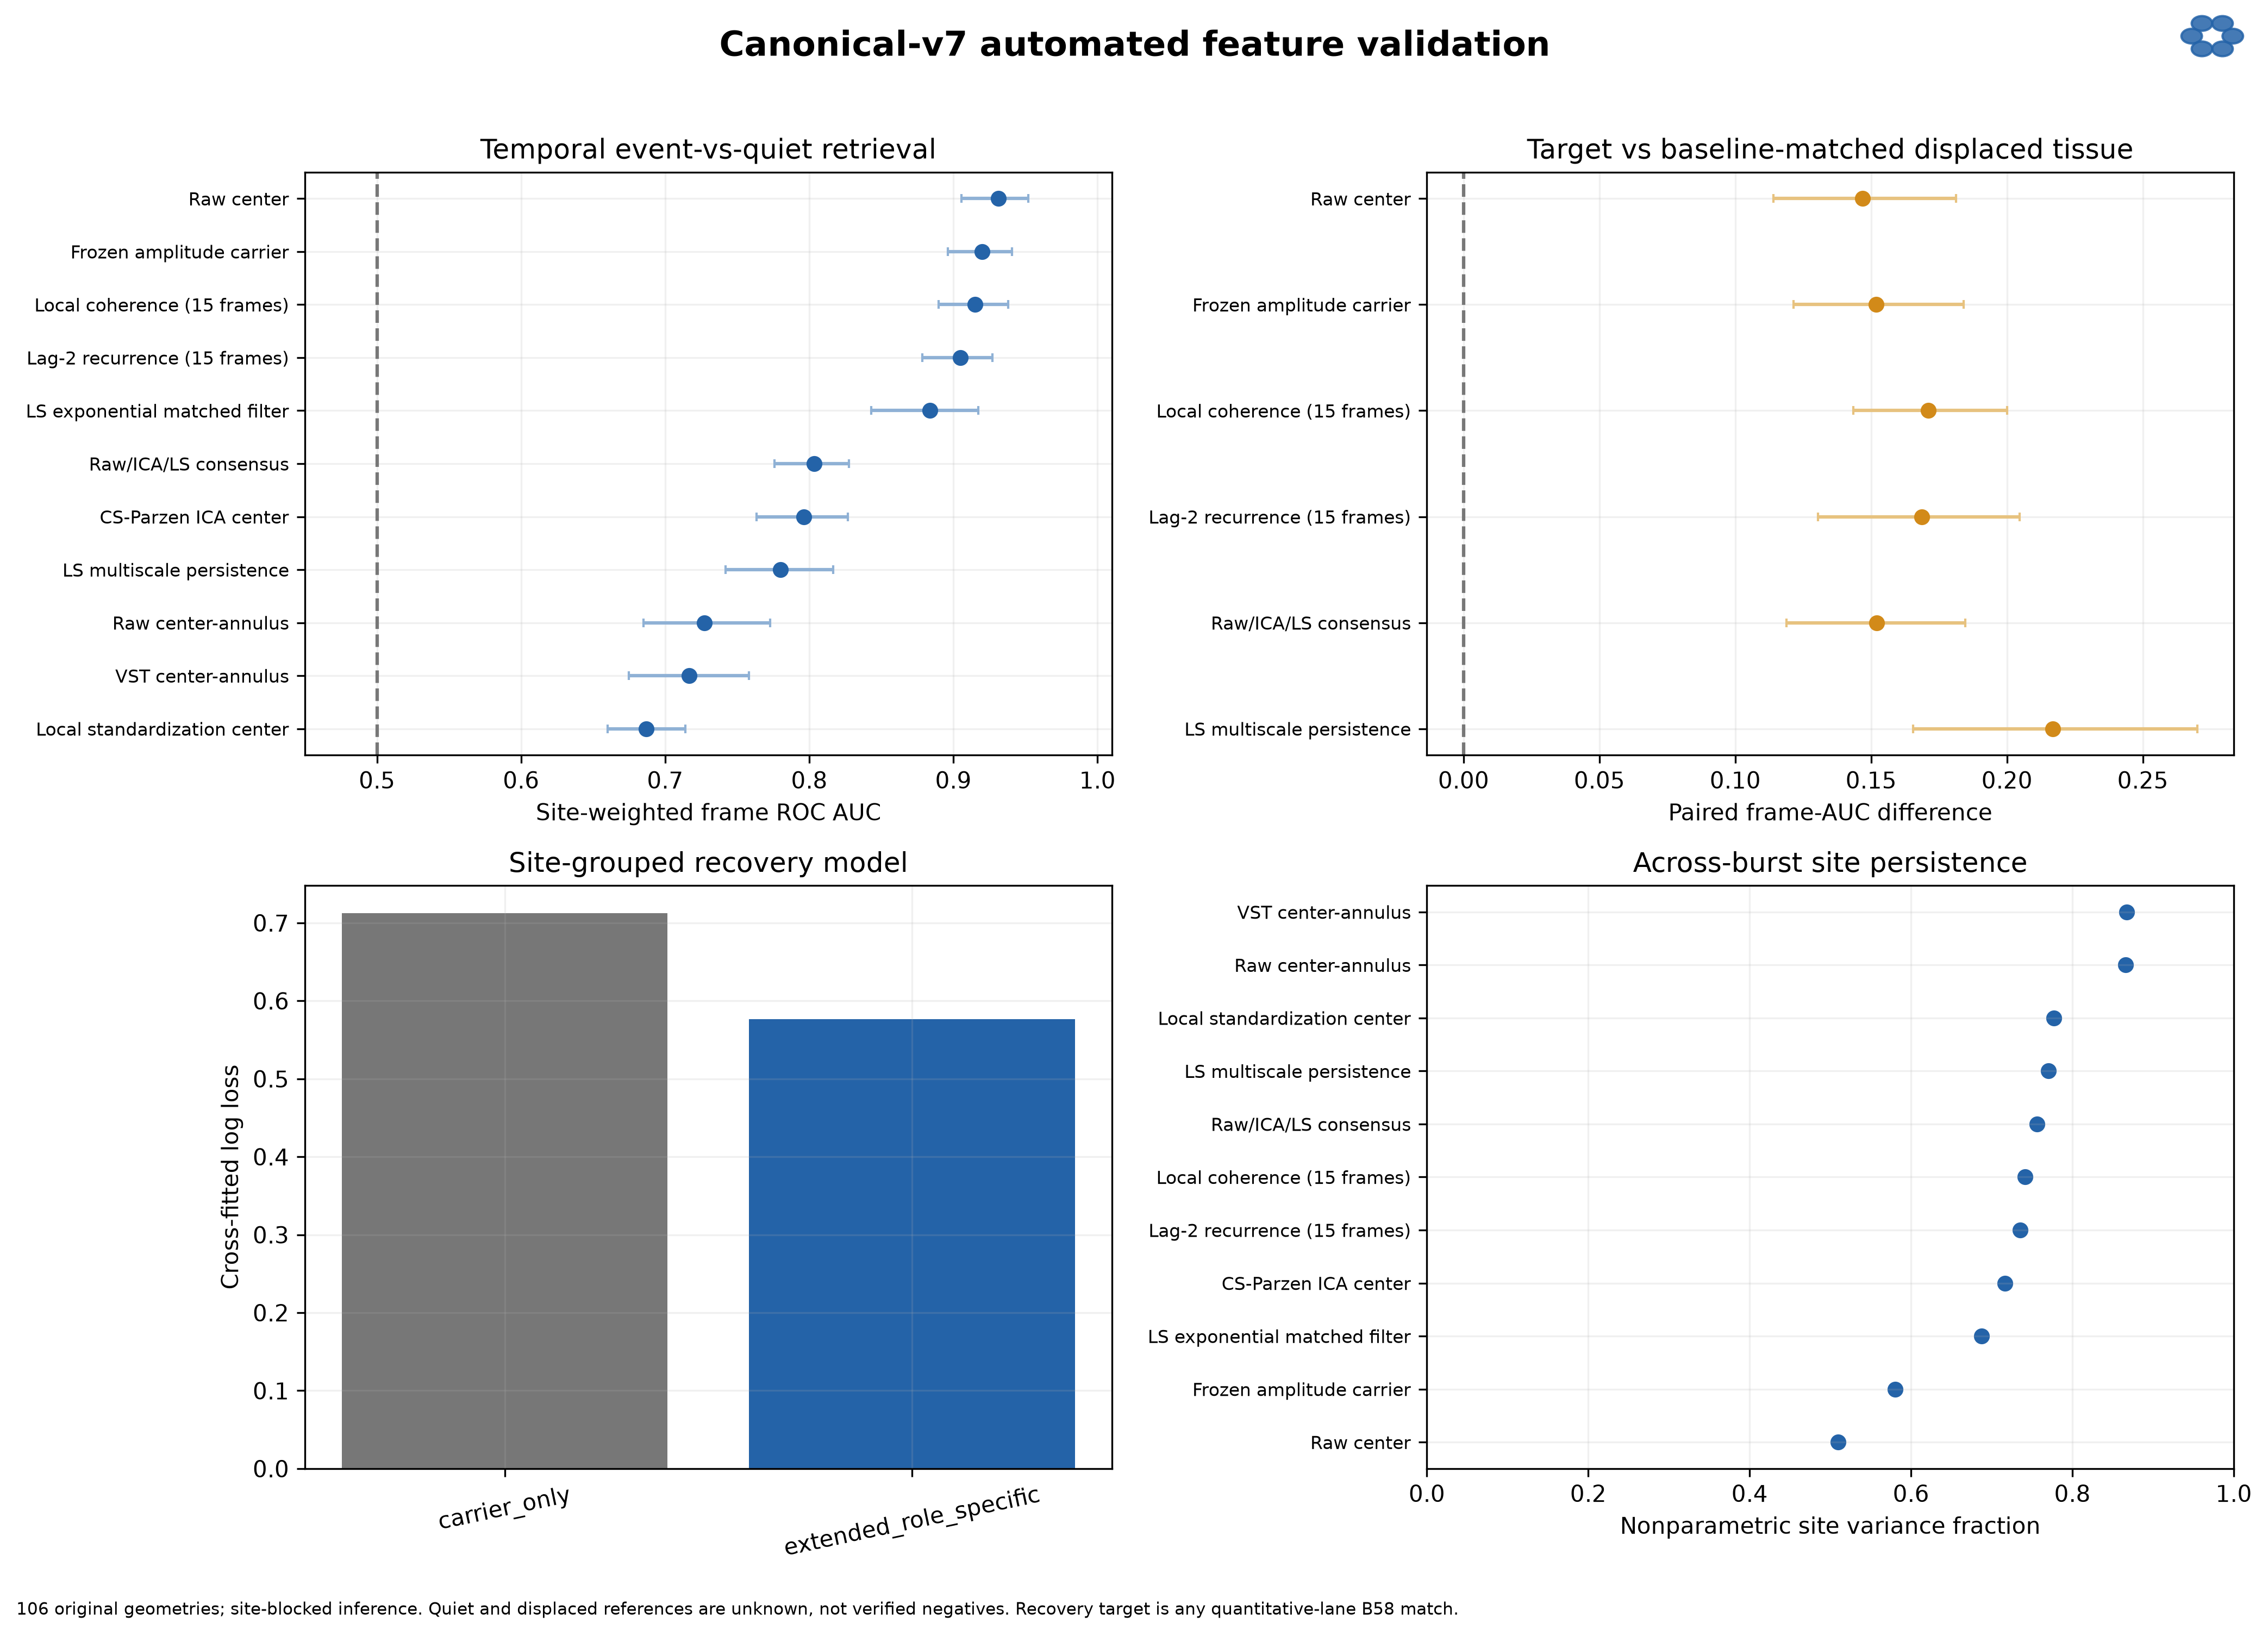
\includegraphics[width=0.98\linewidth]{figures/final/fig09_automated_feature_validation.png}
  \caption{Automated temporal retrieval, spatial displacement, grouped
  recoverability, and repeatability tests. Displaced tissue is an unknown
  control, not a verified negative.}
  \label{fig:automated-feature-validation}
\end{figure}

\begin{figure}[p]
  \centering
  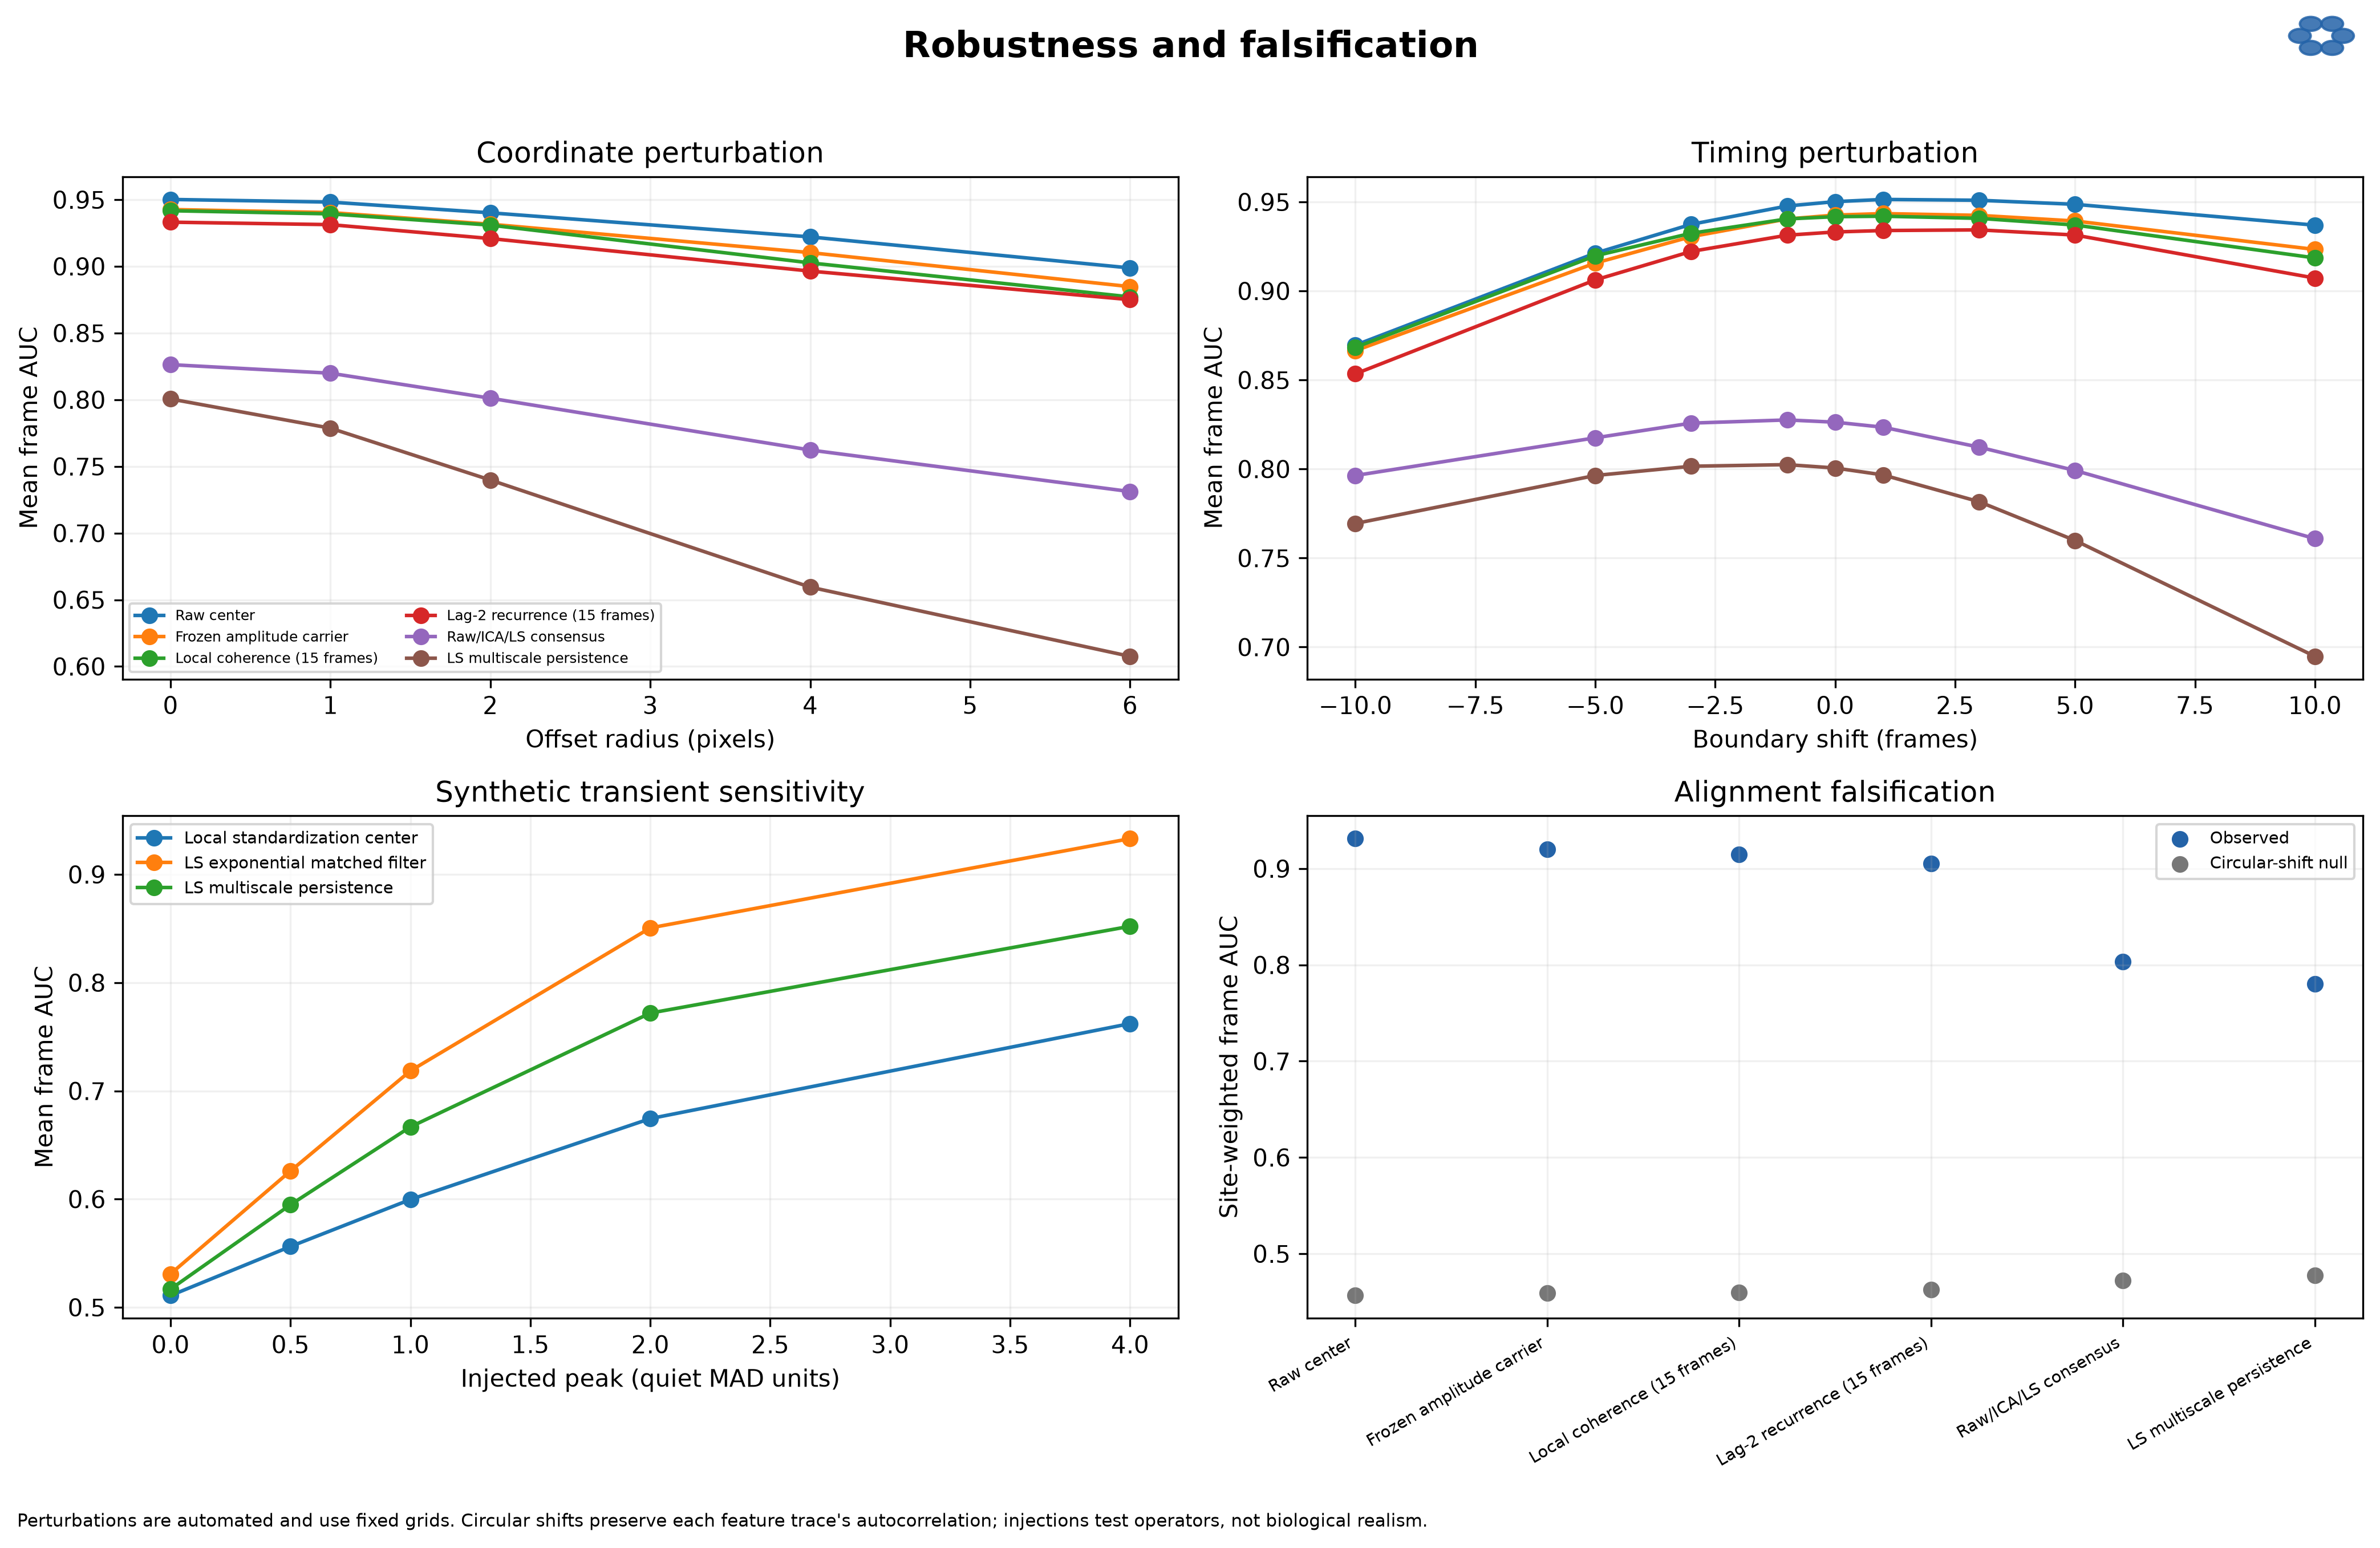
\includegraphics[width=0.98\linewidth]{figures/final/fig10_robustness_falsification.png}
  \caption{Fixed coordinate and timing perturbations, synthetic transient
  sensitivity, and site-blocked circular-shift falsification. The injection is
  one-dimensional and is not a biological or optical simulator.}
  \label{fig:robustness-falsification}
\end{figure}

\subsection{Deep dives separate proposal, ranking, kinetics, and failure modes}

At the frozen B58 operating point, \DeepRecoveredAll{} occurrences were
recovered by all three quantitative lanes, \DeepRecoveredPartial{} by a subset,
and \DeepAllMisses{} by none. Of the all-lane misses, five were uniform
localization misses and four were uniform identity conflicts; the remaining
three involved ranking, non-maximum suppression, or both. Recovered-minus-missed
center-AUC contrasts were positive for carrier, coherence, and lag, but every
site-bootstrap interval crossed zero.

The common-proposal analysis distinguished spatial proposal formation from
ranking on an identical candidate universe. At budget 20, coherence exceeded
carrier by \DeepCoherenceNativeTwenty{} recall in its native proposal stream but
only \DeepCoherenceRankingTwenty{} on common proposals. The corresponding lag-2
contrasts were \DeepLagNativeTwenty{} and \DeepLagRankingTwenty{}. These are
native-versus-common-proposal contrasts, not an additive causal decomposition,
but they indicate that the early-budget value is not explained by reranking
alone.

A fixed calcium-kinetic bank selected \DeepKineticKernel{} in every
leave-one-burst-out fold. Its overall site-weighted frame AUC was
\DeepKineticAUC{}, and the unweighted mean of held-burst AUCs was
\DeepKineticLOBOAUC{}. Across 20 repeated site-grouped splits, compact
carrier/coherence/lag recovery modeling changed log loss from
\DeepCarrierLoss{} to \DeepCompactLoss{}. The broader role-specific model was
stronger in point estimates, but only 12 all-lane misses make all recovery
models exploratory.

\subsection{Canonical-v8 review separates localization gain from identity reassignment}

The identity-aware review changed the interpretation of the 12 all-lane B58
misses without changing the canonical-v7 coordinates or labels. Under the fixed
six-pixel cross-stage consensus search, two response-maximizing candidates
collided with another geometry of the same canonical identity and six collided
with a different canonical identity. Only four candidates---ROI~19, ROI~22,
ROI~25, and ROI~27---were identity-clear within six pixels. Consequently, eight
of 12 apparent local improvements cannot be called coordinate corrections.

The reviewer-suggested ROI~23 shift approached ROI~26, while the ROI~12
consensus landed exactly on ROI-new-002 and the suggested shift lay 2.24 pixels
from it. ROI~10 and ROI~15 formed a same-canonical-identity cluster, and all
three ROI~11 occurrences shifted toward ROI-new-001. Among the identity-clear
cases, ROI~22 remained noise-dominated, ROI~19 was plausible but noise-limited,
ROI~27 retained a credible crowded-field transient consistent with
non-maximum-suppression failure, and ROI~25 remained a noisy ranking case. This
canonical-v8 result is a reviewed failure-interpretation update, not a revised
truth set or evidence of one-to-one biological source recovery.

The strict detector result therefore remains $94/106=88.7\%$, and the existing
canonical-collapsed sensitivity remains $93/102=91.2\%$
(\Cref{tab:identity-aware-v8}). Excluding the eight collision occurrences gives
an audit-conditioned $94/98=95.9\%$ sensitivity among currently
identity-resolved occurrences, but this is not an updated detector recall. Even
if all four identity-clear hypotheses were later validated and recovered, the
corresponding strict-recall ceiling would be $98/106=92.5\%$. Neither
sensitivity licenses counting an identity collision as a detection.

\begin{table}[!htbp]
\centering
\caption{Canonical-v8 identity-aware interpretation of the frozen B58 recovery
result. Only strict recall is an official detector metric. Audit-conditioned
and hypothetical values are sensitivities, not replacement performance
estimates.}
\label{tab:identity-aware-v8}
\small
\begin{tabularx}{\linewidth}{>{\raggedright\arraybackslash}p{0.31\linewidth} >{\raggedright\arraybackslash}p{0.20\linewidth} X}
\toprule
Quantity & Value & Interpretation \\
\midrule
Strict recovered occurrences & $94/106=88.7\%$ & Frozen official known-positive recall; unchanged by v8. \\
Canonical-collapsed sensitivity & $93/102=91.2\%$ & Existing duplicate-collapsed sensitivity; unchanged by v8. \\
All-lane misses & $12/106=11.3\%$ & Frozen miss count entering the identity-aware audit. \\
Same-identity collisions & $2/12=16.7\%$ & Candidate approaches another geometry assigned to the same canonical identity. \\
Different-identity collisions & $6/12=50.0\%$ & Candidate approaches a different labeled canonical identity. \\
Identity-clear hypotheses & $4/12=33.3\%$ & ROI 19, 22, 25, and 27 remain unresolved localization, noise, ranking, or NMS hypotheses. \\
Identity-resolved conditional sensitivity & $94/98=95.9\%$ & Descriptive sensitivity after excluding eight collision occurrences from the evaluable denominator; not official recall. \\
Four-case rescue ceiling & $98/106=92.5\%$ & Hypothetical strict recall if every identity-clear candidate were independently validated and recovered. \\
\bottomrule
\end{tabularx}
\end{table}


The automated identity-aware feature panel then tested cross-stage offset
stability, point/disk/footprint extraction, response-footprint morphology,
local competition, and neighboring-trace leakage without fitting a classifier
to the four identity-clear misses (\Cref{fig:identity-aware-features}). Median
pairwise offset-direction cosine was 0.972 for collision cases versus 0.448 for
identity-clear misses, while median offset-vector spread was 1.13 versus 1.83
pixels. This is consistent with a strong neighboring source pulling multiple
representations in the same direction; it is not evidence that the collision
coordinate belongs to the missed identity.

Local-standardized candidate traces also retained more neighboring-trace
structure in collision cases. Median candidate--neighbor partial correlation
after removing the original-center trace was 0.474 for collisions and 0.182
for identity-clear misses; median nonnegative neighbor weight was 0.460 versus
0.187. ROI~12 was the limiting example, with partial correlation and neighbor
weight both equal to 1.0 at the candidate that coincided with ROI-new-002.

Footprint morphology was not a strong separator: median eccentricity was 0.774
for collisions and 0.810 for identity-clear misses, with median solidity 0.781
and 0.714. Response-weighted extraction increased median local-standardized
event peak relative to pre-event MAD from 4.06 to 22.99 in collision cases and
from 3.97 to 12.67 in identity-clear misses. Because the footprint weights were
selected from the same event response, these gains establish extraction
sensitivity rather than prospective recovery or identity specificity.

Among identity-clear cases, ROI~19 had perfectly aligned stage offsets and low
neighbor leakage, making it the cleanest localization hypothesis despite weak
spatial support. ROI~25 also had consistent offsets and low leakage but an
irregular footprint. ROI~22 and ROI~27 had inconsistent stage offsets, favoring
noise or crowded-field instability over a stable point correction.

The broader frozen validation suite strengthened the proposal-absence
interpretation. No identity-clear miss had a frozen candidate within eight
pixels by budget 100 in any carrier, coherence, or lag lane. These cases are
therefore not merely B58 ranking failures in the audited candidate inventory.
Collision cases retained some nearby candidates because the inventory can
approach the competing identity. Leave-one-stage-out candidate gain was 1.54
for collisions and 1.31 for clear misses, but the exact occurrence-grain
permutation value was 0.371.

Multi-neighbor fits explained median 52.3\% of collision-candidate variance
versus 8.8\% for clear misses. After subtracting neighboring traces, median
event peak/MAD was 4.02 versus 5.48. Pre-event-frozen footprints retained
median peak/MAD 11.98 and 9.51, respectively, demonstrating prospective
within-recording extraction sensitivity without target-event footprint
selection. Recovered-site response maximization shifted a median 2.24 pixels,
while quiet pseudo-events shifted 5 pixels, confirming that unconstrained
recentring itself creates displacement. Cross-burst transfer produced 34
collision source--target pairs but only one clear pair and therefore could not
compare the groups. None of three exact eight-versus-four descriptive tests
was small ($p=0.371$, 0.169, and 0.308).

\subsection{Expanded automated tests prioritize observability context and abstention}

Ten additional frozen test families evaluated identity-grouped prediction,
site-bootstrap stability, conditional importance, prospective transfer,
controlled mixtures, metamorphic behavior, selective risk, recovered-only
anomaly detection, and graph crowding (\Cref{fig:expanded-automated-v3}). The
full panel reached identity-grouped ROC AUC 0.833 and log loss 0.498, compared
with AUC 0.611 and log loss 0.690 for carrier alone. These values strengthen
within-recording error stratification rather than establish generalization.

Across 100 site-bootstrap sparse fits, variance-stabilized center-annulus was
selected in 97\%, multiscale persistence in 73\%, lag-2 recurrence in 39\%, and
the matched filter in 29\%. Within-burst conditional permutation increased log
loss by 0.0484, 0.0244, and 0.0234 for the first three features. The annular
result is not necessarily neural: its weak event retrieval and high stability
indicate persistent observability, background, or acquisition context.

Confidence-based abstention reduced internal error from 20.8\% at full coverage
to 9.4\% at 50\% coverage. Recovered-only isolation-forest and robust-distance
scores separated misses with AUC 0.814 and 0.760. A simple five-neighbor graph
statistic had negligible association with recovery ($r=-0.009$), showing that
distance-only crowding is inadequate. Controlled mixtures and metamorphic
checks behaved directionally: neighboring transients could inflate peak/MAD,
common mode reduced event contrast while increasing lag recurrence, frozen
intensity scaling preserved peak/MAD, and temporal shifts changed fixed-window
retrieval. These one-dimensional checks validate operators, not movie
formation.

\begin{figure}[p]
  \centering
  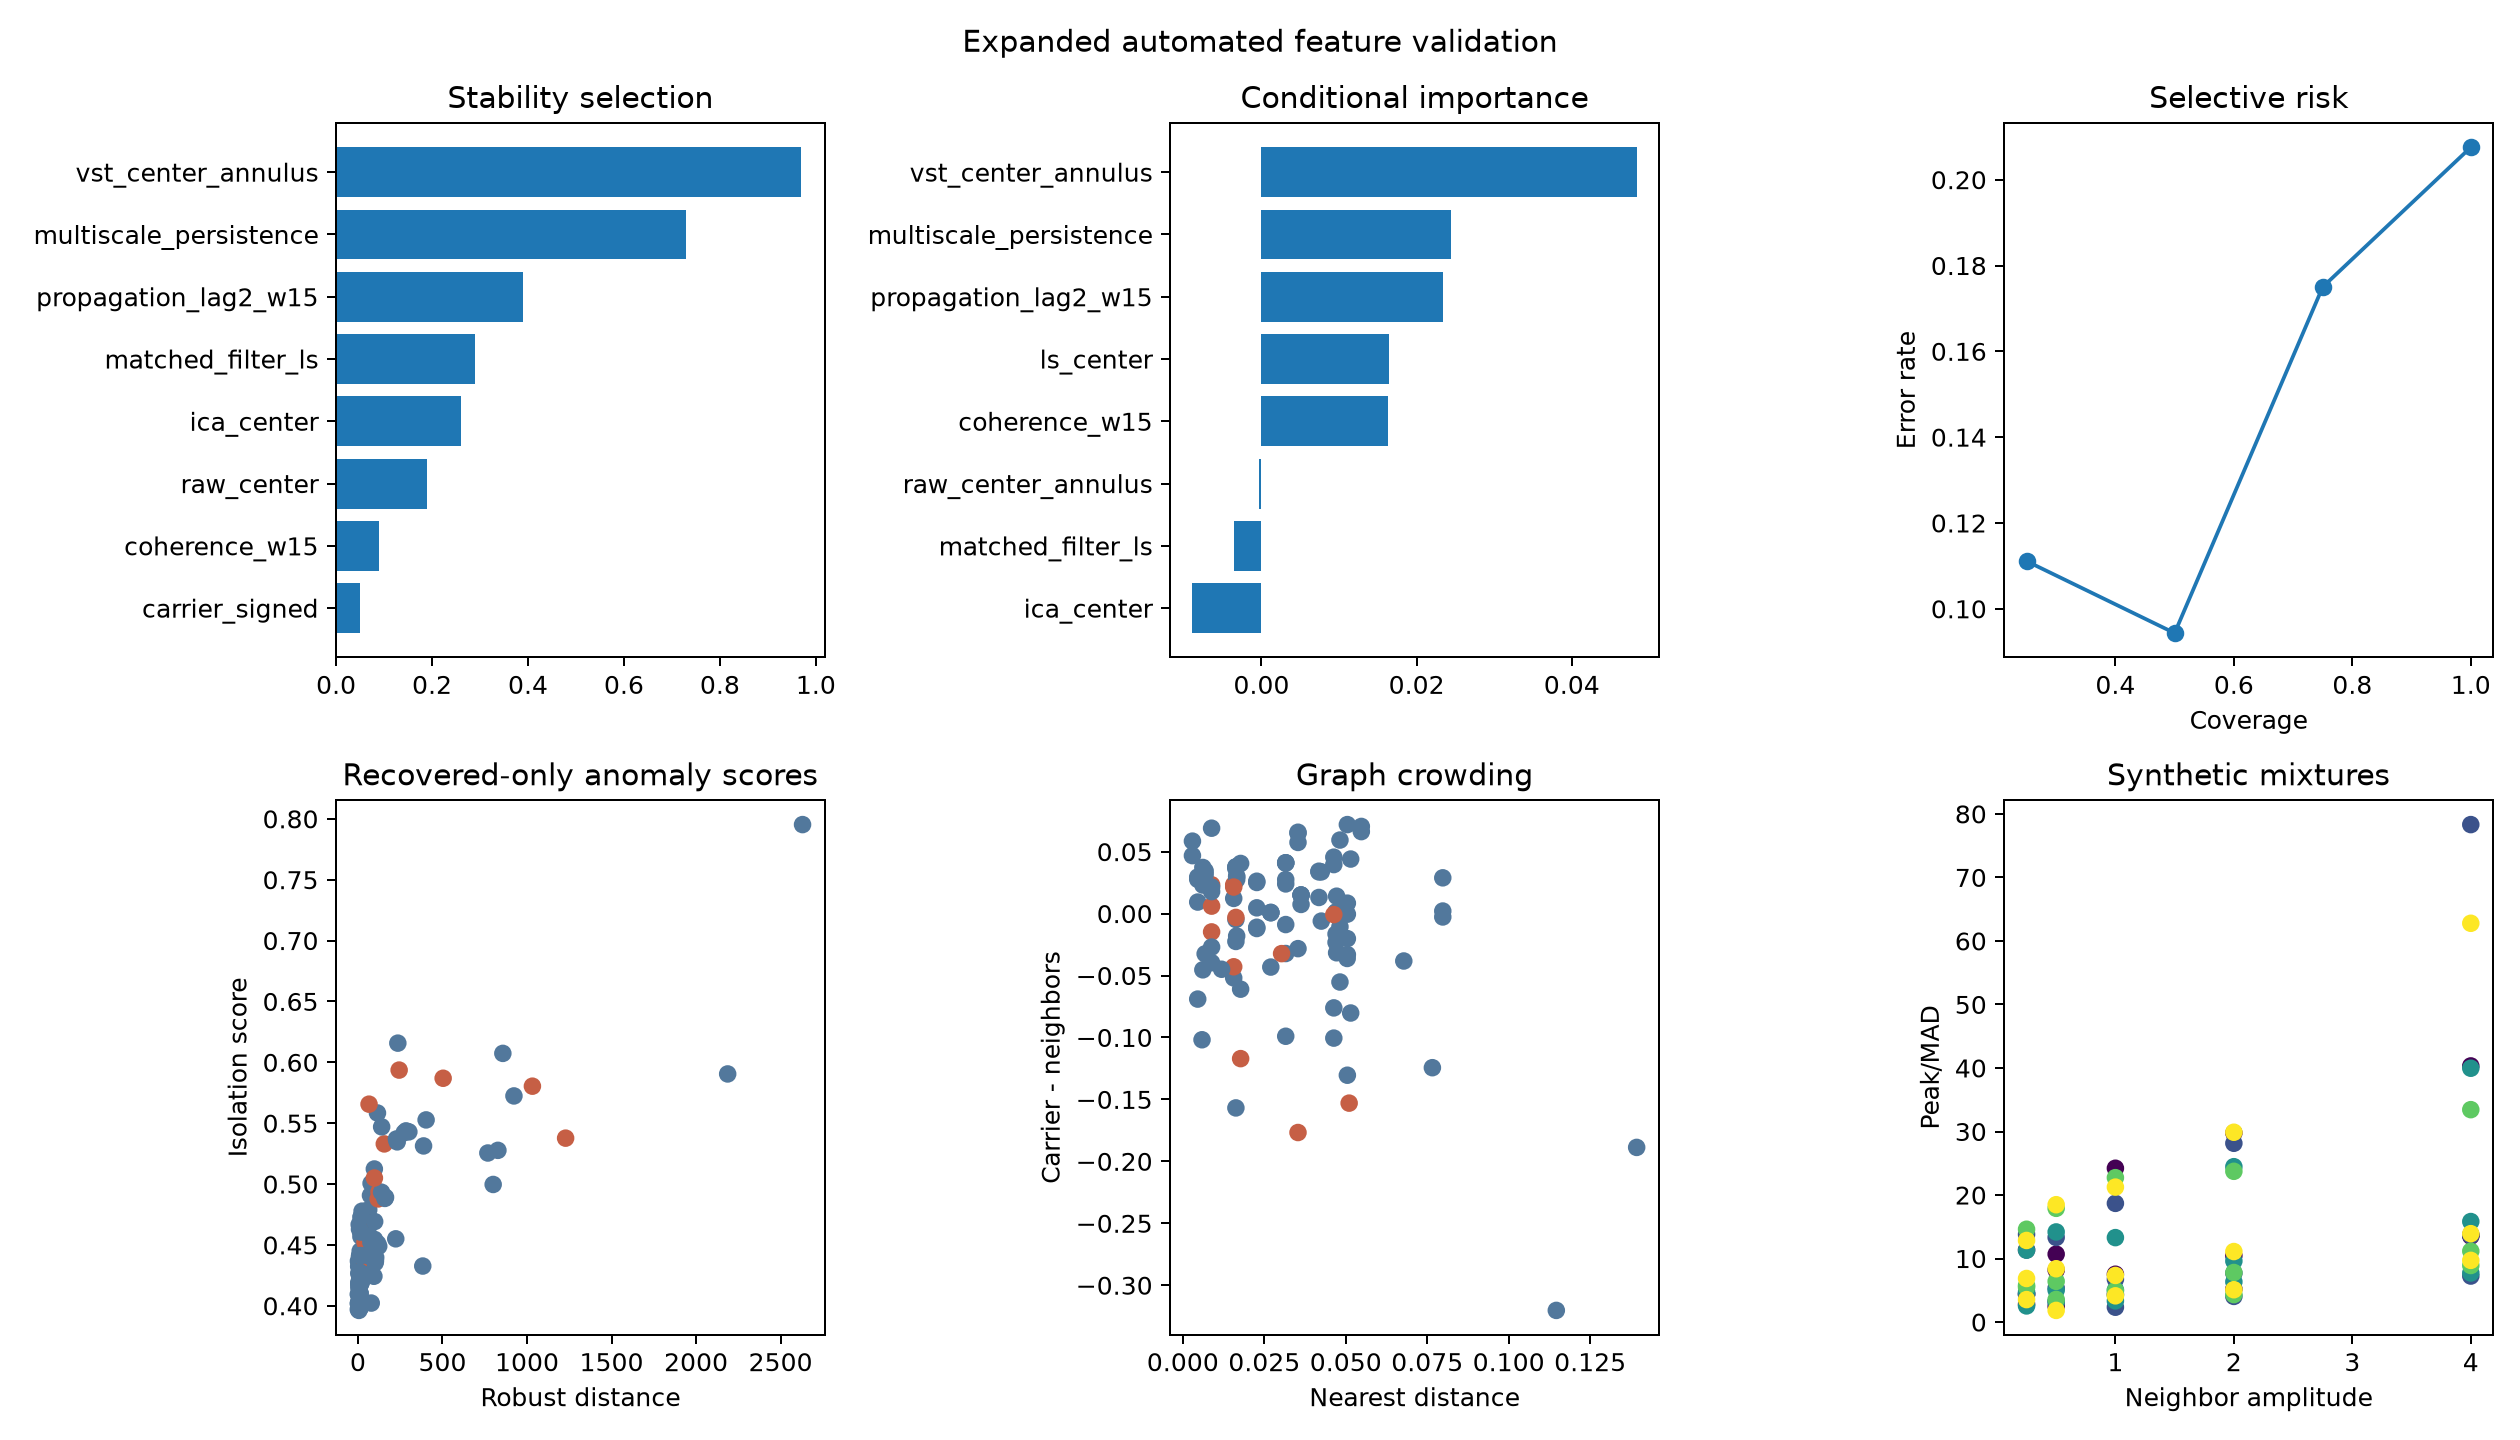
\includegraphics[width=0.99\linewidth]{figures/final/fig14_expanded_automated_validation.png}
  \caption{Expanded automated validation. Stability, importance, selective
  risk, anomaly, graph, and synthetic panels are exploratory within one
  recording; unmatched candidates remain unknown and synthetic mixtures are
  one-dimensional.}
  \label{fig:expanded-automated-v3}
\end{figure}

\begin{figure}[p]
  \centering
  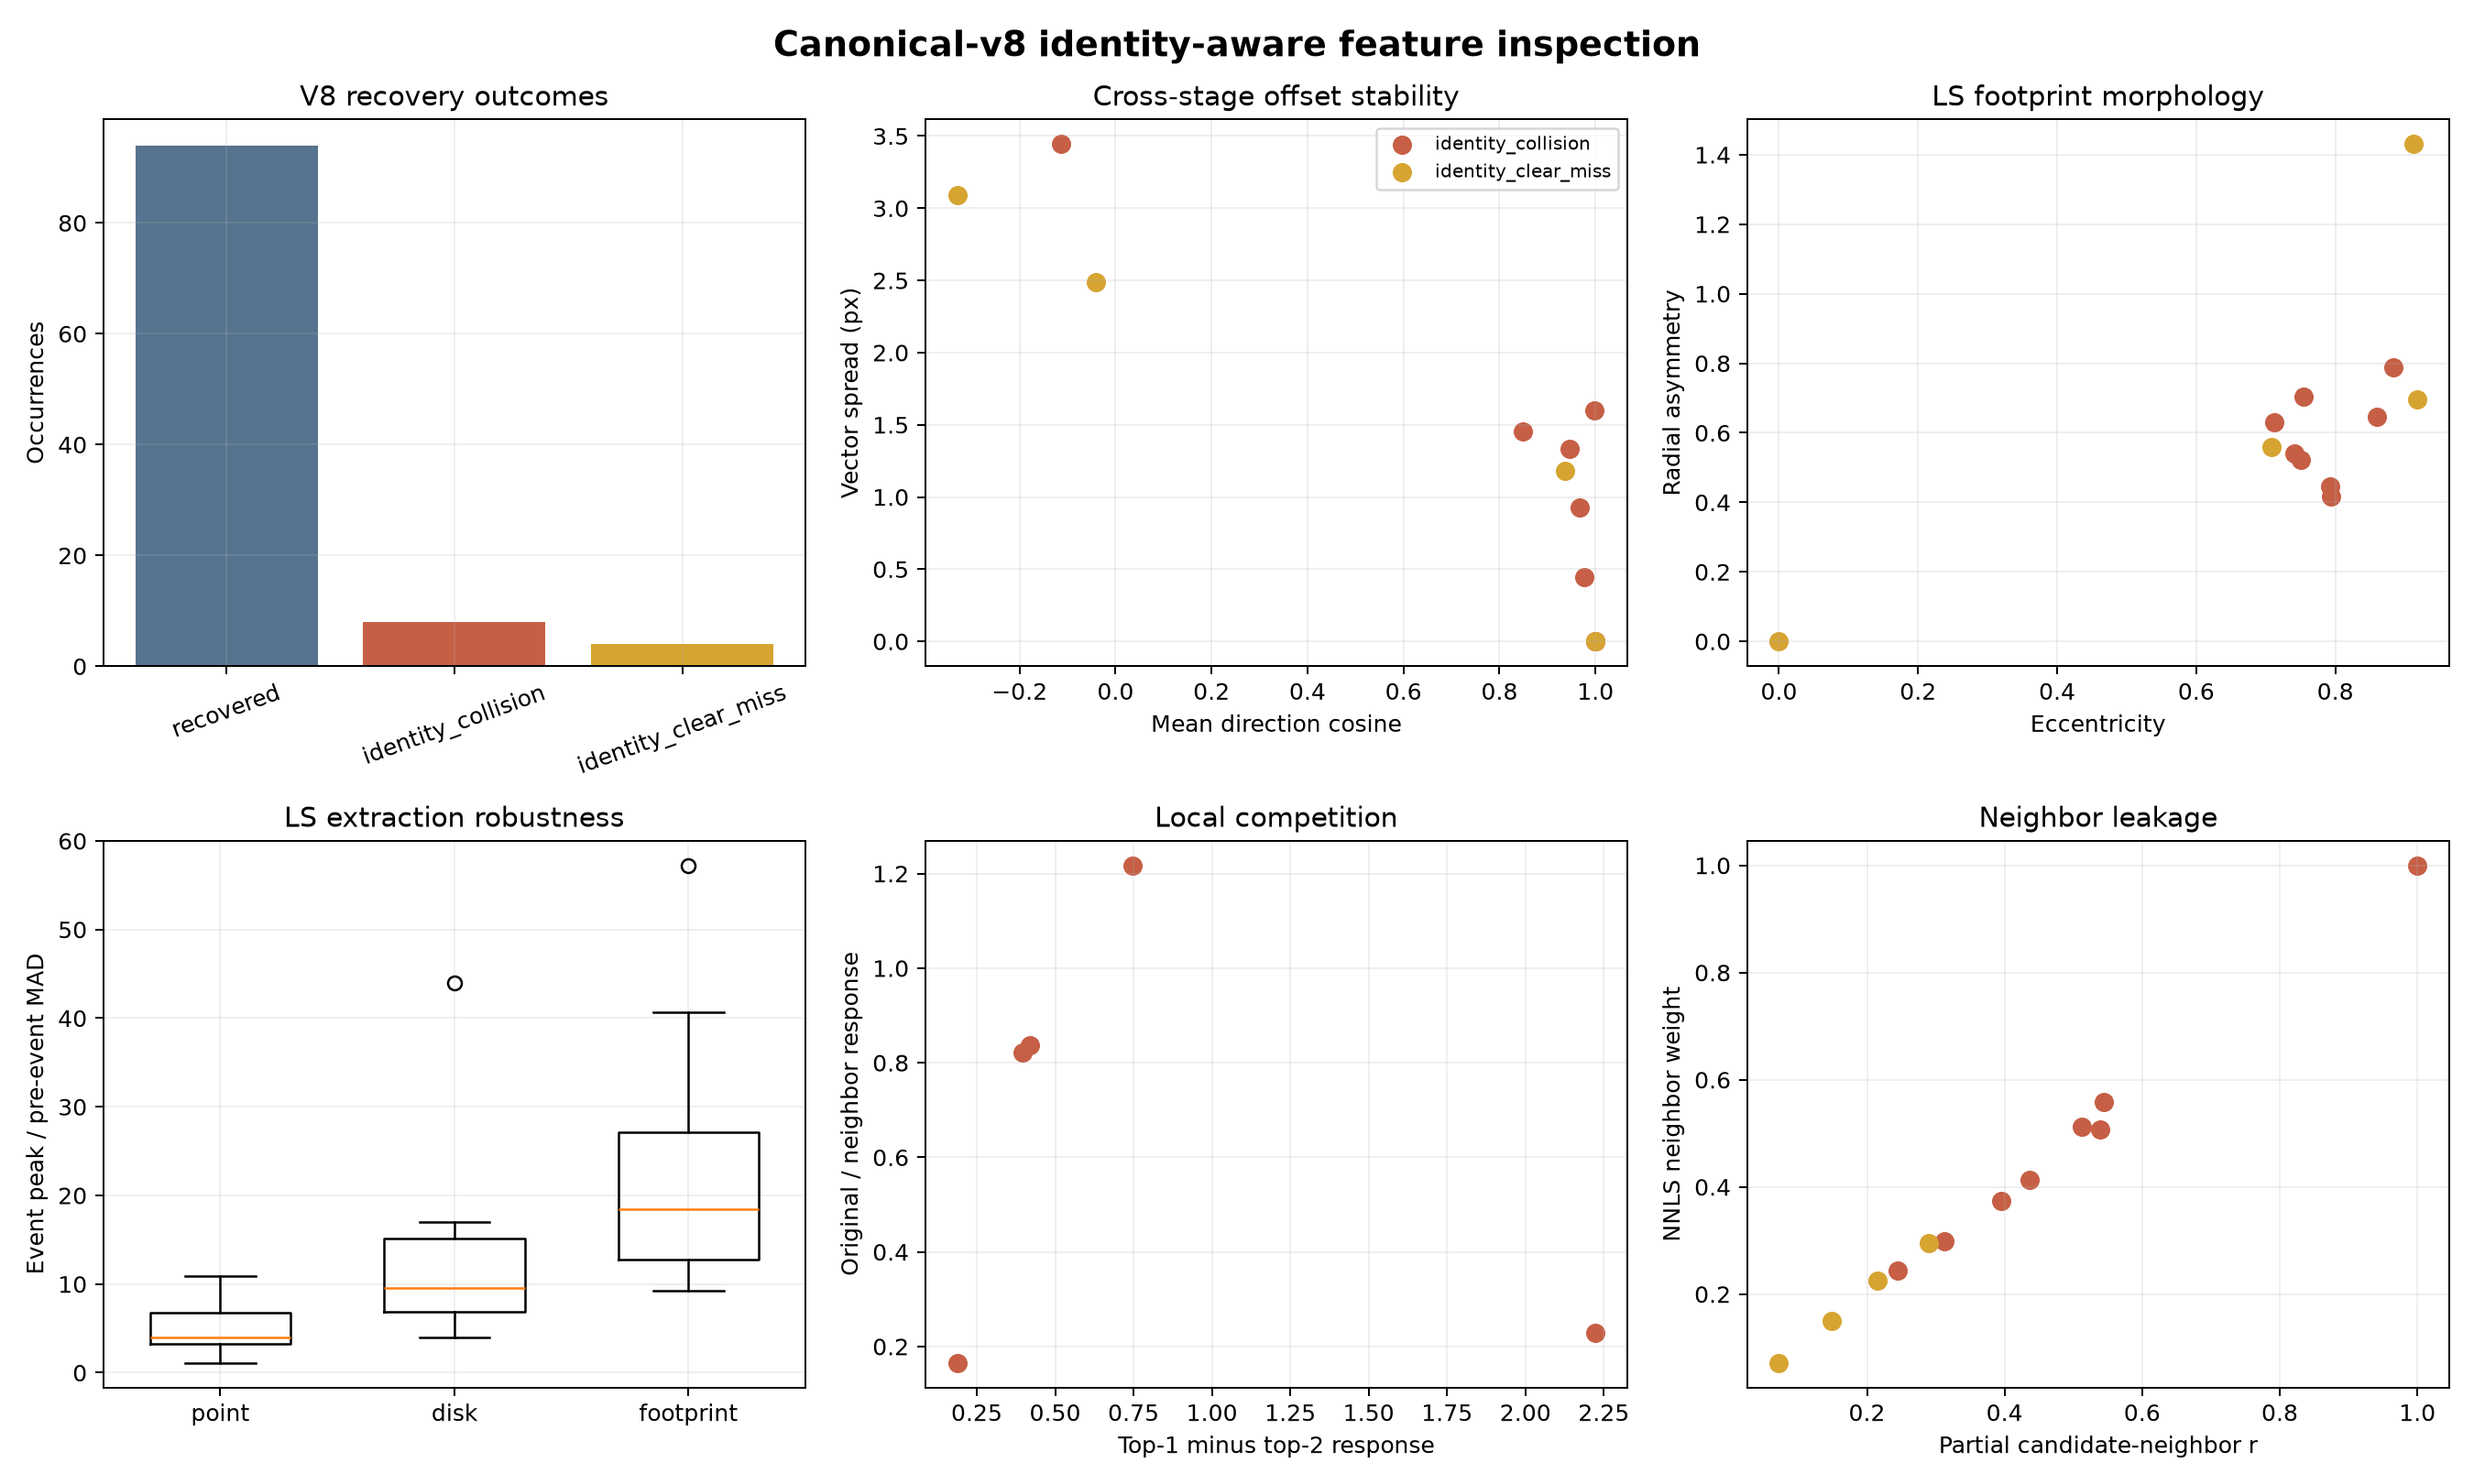
\includegraphics[width=0.99\linewidth]{figures/final/fig13_identity_aware_feature_inspection_v8.png}
  \caption{Canonical-v8 identity-aware feature inspection. The three-outcome
  panel is descriptive; collision and identity-clear groups contain eight and
  four misses. Footprint extraction is response-selected from the same events,
  and nearest labeled geometry is not exhaustive biological truth.}
  \label{fig:identity-aware-features}
\end{figure}

\begin{figure}[p]
  \centering
  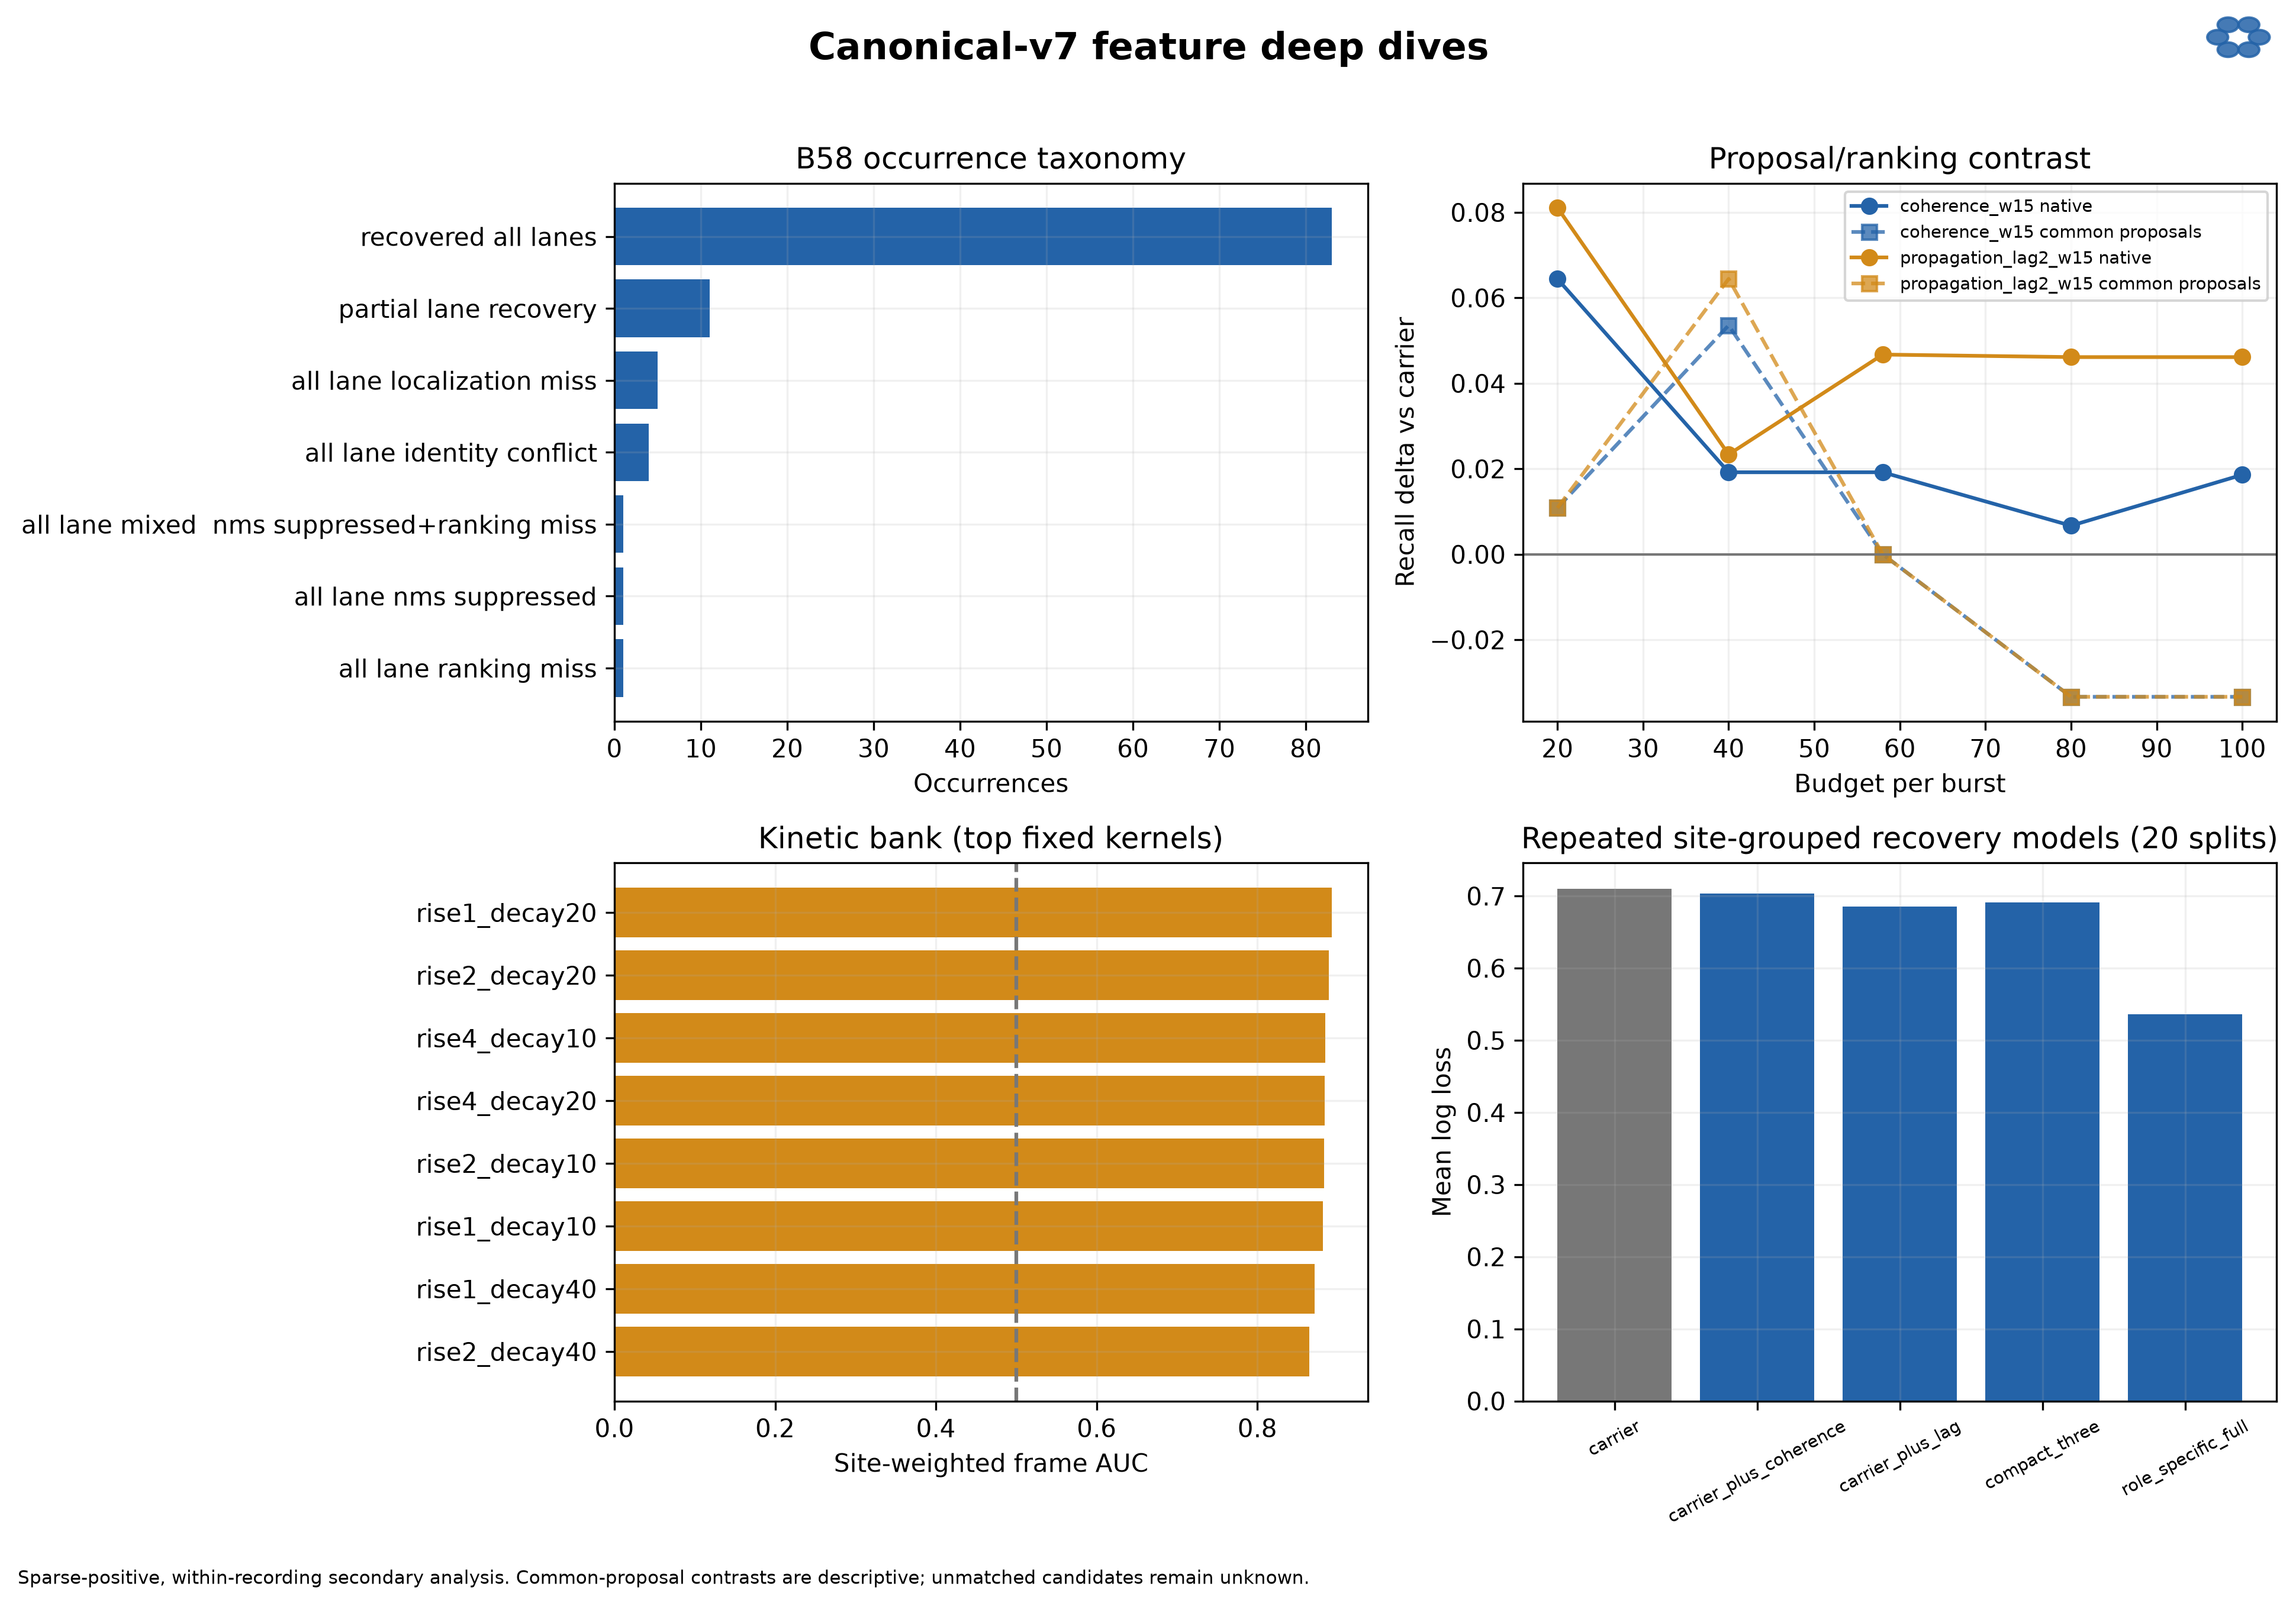
\includegraphics[width=0.98\linewidth]{figures/final/fig11_feature_deep_dives.png}
  \caption{Prespecified feature deep dives: exact B58 failure taxonomy,
  native-versus-common-proposal contrasts, a fixed kinetic filter bank, and
  repeated site-grouped recovery models. Sparse positives and small failure
  counts limit interpretation.}
  \label{fig:feature-deep-dives}
\end{figure}

\begin{figure}[!htbp]
  \centering
  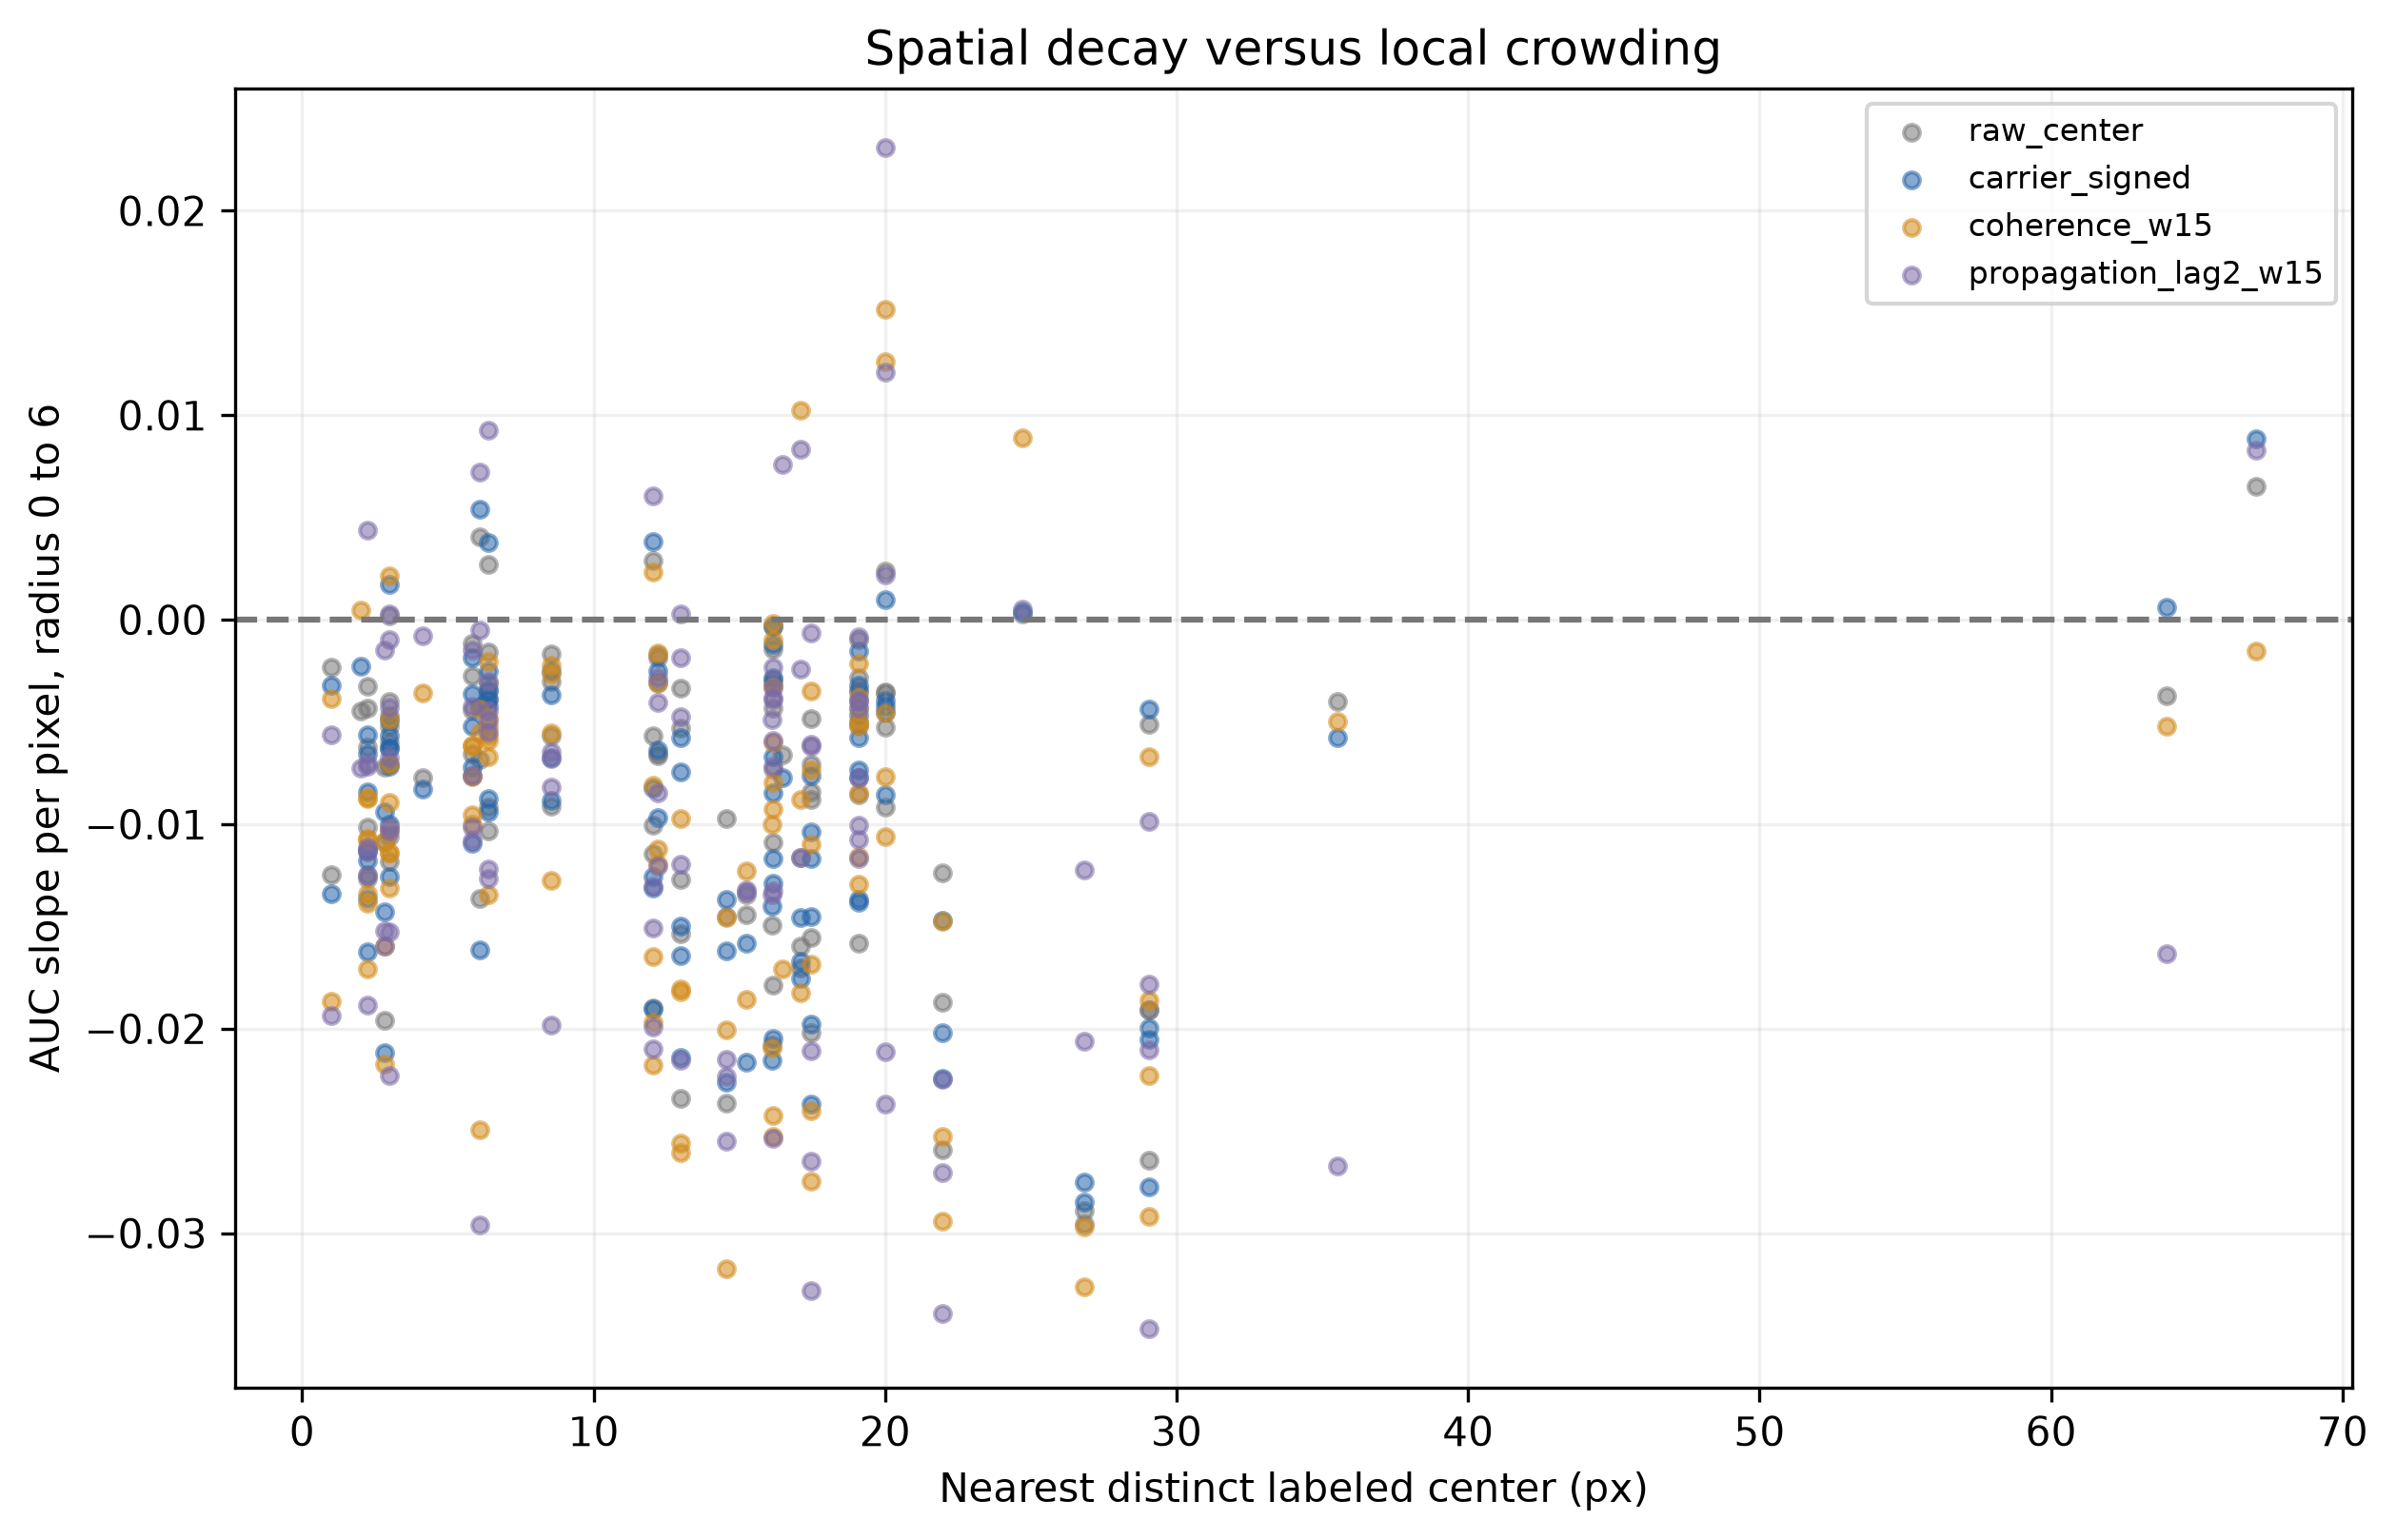
\includegraphics[width=0.86\linewidth]{figures/final/fig12_spatial_decay_crowding.png}
  \caption{Radius-0-to-6 retrieval decay versus the nearest distinct labeled
  center. Duplicate burst occurrences at one immutable site are not counted as
  spatial neighbors; labeled-center density is an incomplete crowding proxy.}
  \label{fig:spatial-decay-crowding}
\end{figure}

\DraftFigure{Recall-versus-candidate-budget curves for the frozen representation panel, proposal-union ceilings, same-proposal ranking comparisons, and failure categories. A separate panel will report bounded-field precision--recall after blinded exhaustive review.}{Detection implications under positive--unlabeled annotation.}{fig:detection-implications}

\subsection{Acquisition structure is a potential determinant of observability}

Preliminary quiet-frame analysis reported an intensity--variance slope of approximately \QuietVarianceSlope{} with weighted $R^2$ between \QuietVarianceWeightedRtwo{}. The audit also identified a provisional field boundary near \ProvisionalFieldBoundaryX{} and a left--right global-trace correlation of \LeftRightGlobalCorrelation{}. These observations motivate stratification by field, saturation, baseline intensity, motion, and local effective rank. The final analysis will determine whether recurrently difficult sites are explained by biological event magnitude, acquisition position, local contamination, or a combination of these factors.

\DraftFigure{Variance-versus-intensity fit, saturation and motion maps, field-boundary diagnostics, temporal spectra, and a comparison of the canonical recording with any available unlabeled recordings.}{Acquisition physics and recording-quality context.}{fig:acquisition-qc}

\subsection{Detection occurrences form recurring measurement-profile classes}

The maximum-filter audit revealed that flat feature-map plateaus could contribute adjacent pixels to a nominal non-maximum-suppressed candidate list. We therefore repeated the frozen analysis with explicit Euclidean object separation and a label-free event-maximum tie breaker. Both compact lanes retained their positive known-positive-recall gains across the prespecified 4, 6, and 8 pixel sensitivity settings. At the primary 6 pixel, budget-20 operating point, the cross-lane union contained 86 distinct detection occurrences at 36 consolidated spatial detection sites.

We constructed an 11-variable profile for every detection occurrence using native and residual peak amplitude, robust signal-to-noise ratio, spatial specificity, annulus coupling, signed event area, relative peak time, lane agreement, candidate rank, cross-burst recurrence, and quiet intensity. Continuous measurement features were robustly standardized within burst so that clustering would not merely reproduce burst intensity. Expert labels were excluded from fitting. Candidate solutions with two through six classes were compared using silhouette separation and bootstrap adjusted Rand stability, with a minimum of five occurrences and two bursts per class. The selected three-class solution had silhouette 0.284 and mean bootstrap adjusted Rand index 0.724; every class occurred in all four bursts.

\begin{table}[!htbp]
\centering
\caption{Frozen label-free detection-profile classes. Medians are reported in native intensity units where applicable. Known-positive overlap is descriptive only and is not precision.}
\label{tab:detection-profile-classes}
\small
\begin{tabular}{p{0.29\linewidth}rrrrr}
\toprule
Class & Occurrences & Sites & Raw peak & Residual peak & Spatial specificity \\
\midrule
Localized, high-signal, recurrent & 35 & 12 & 618.7 & 280.4 & 0.319 \\
Broad, low-signal, early/episodic & 8 & 6 & 269.5 & 94.0 & 0.170 \\
Broad, lower-signal, recurrent & 43 & 24 & 271.6 & 97.2 & 0.192 \\
\bottomrule
\end{tabular}
\end{table}


\begin{figure}[!htbp]
  \centering
  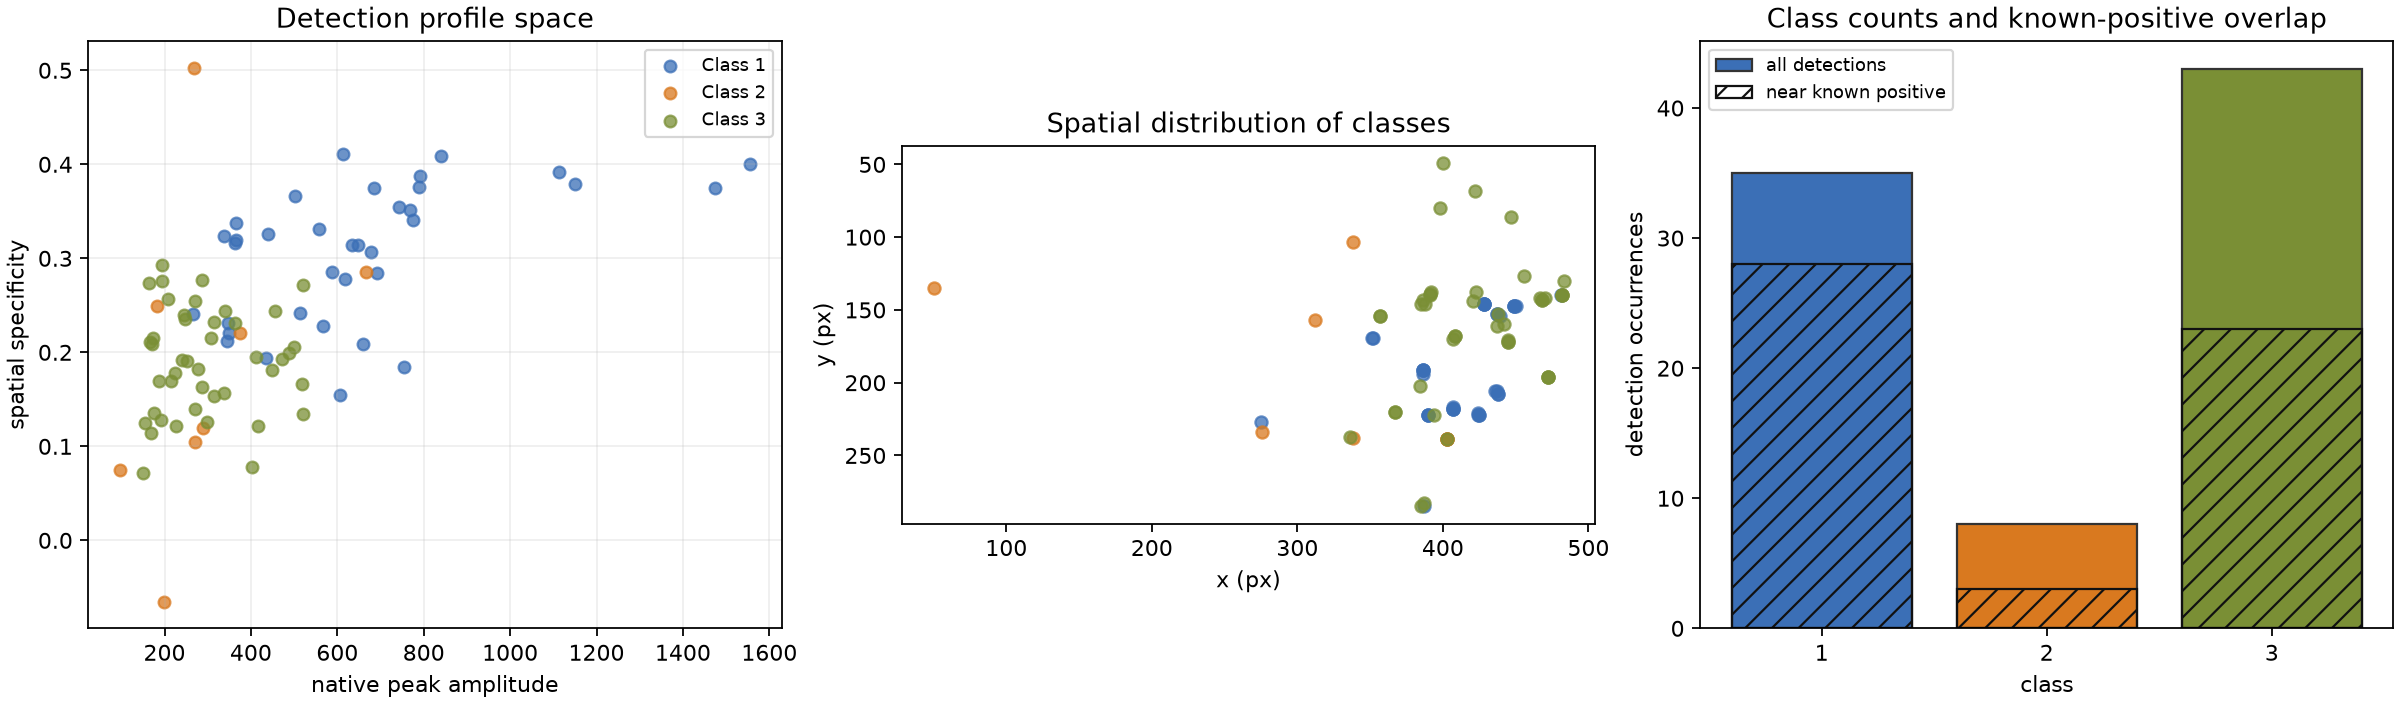
\includegraphics[width=0.98\linewidth]{figures/final/detection_class_overview.png}
  \caption{Label-free detection-profile taxonomy. Points are distinct strict-NMS detection occurrences. Class fitting did not use expert labels; hatched counts show post-freeze proximity to a sparse known-positive annotation and must not be interpreted as precision.}
  \label{fig:detection-profile-overview}
\end{figure}

\begin{figure}[!htbp]
  \centering
  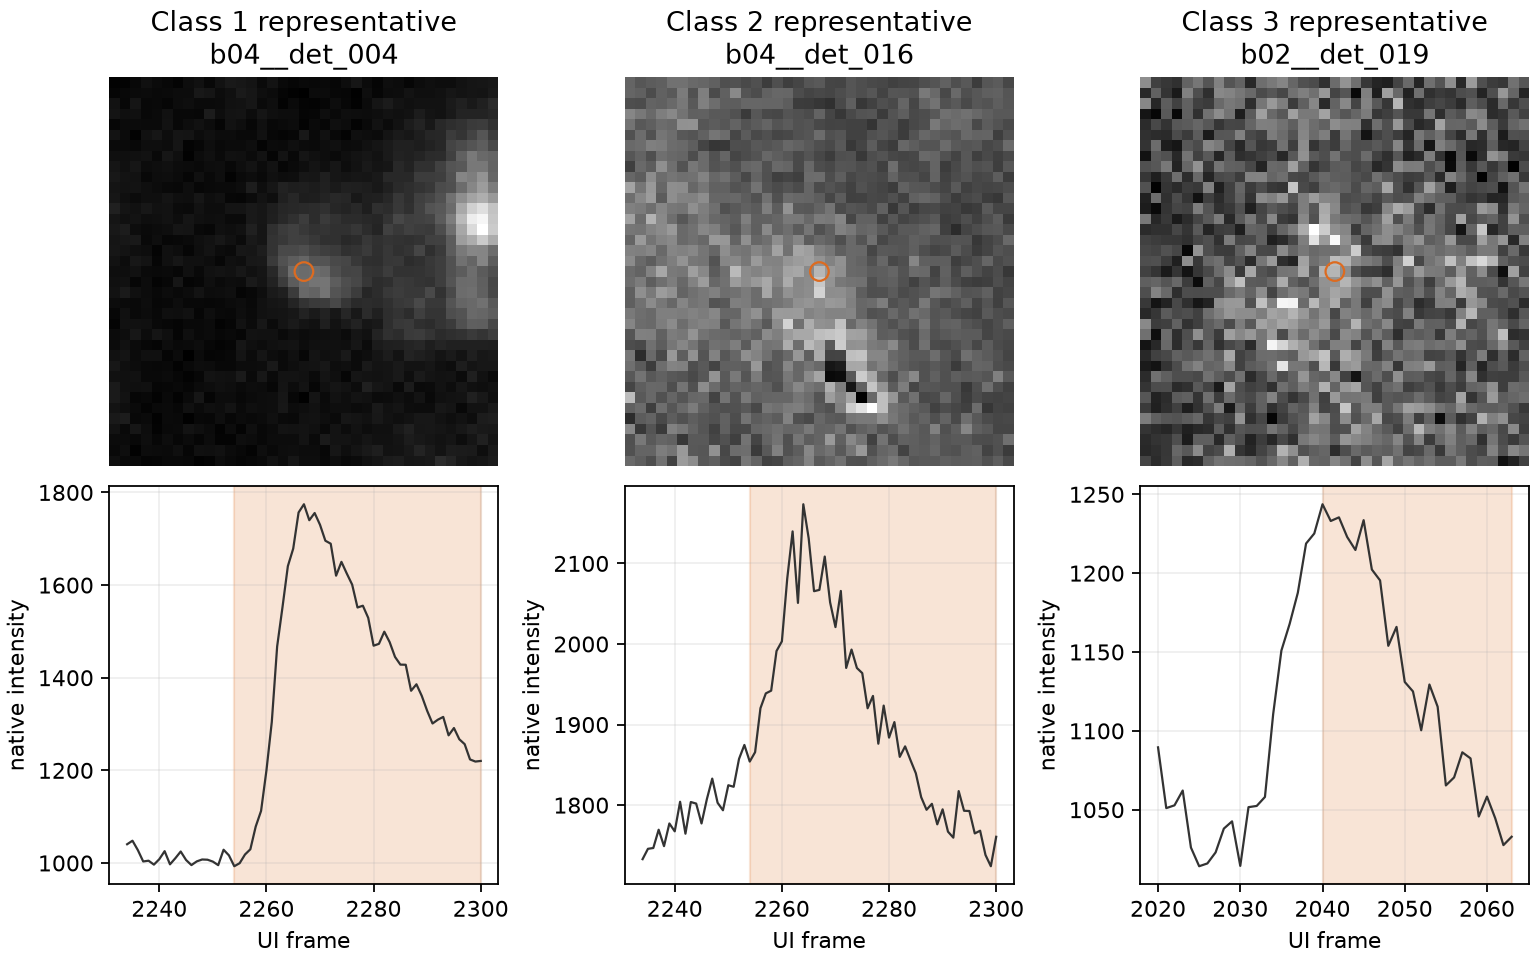
\includegraphics[width=0.98\linewidth]{figures/final/detection_class_representatives.png}
  \caption{Representative occurrence nearest each frozen class centroid. The top row shows event-maximum minus pre-event baseline crops; the bottom row shows native exact-site traces with the evaluated burst interval shaded. Classes describe measurement events, not biological cell types.}
  \label{fig:detection-profile-representatives}
\end{figure}

The largest localized, high-signal class contained 35 occurrences and showed the greatest overlap with sparse known positives (28 occurrences). The broad, low-signal early-peaking class contained eight occurrences, and the broad, lower-signal recurrent class contained 43. These overlap counts characterize already frozen classes; unmatched detections remain unknown rather than negative. The result supports discussion of recurring detection-event archetypes while preserving the positive--unlabeled boundary.

We next joined the frozen classes to adjudicated identity certainty without refitting or renaming the classes. In the frozen-v1 adjudicated subset, the strict budget-20 union matched 10 of 19 confirmed observations but none of five identity-uncertain observations (two-sided Fisher exact $p=0.053$); the single probable observation was retained as a separate category. This small subset suggests a possible observability gradient but is insufficient for a stable class-composition comparison. In expanded canonical v7, the union matched 34 of 54 confirmed and 10 of 22 identity-uncertain observations (Fisher exact $p=0.203$). Thus the expanded data do not establish a difference in overall detection coverage by certainty.

At the occurrence grain, confirmed observations contributed 8, 2, and 24 matches to Classes 1--3, whereas identity-uncertain observations contributed 0, 4, and 6. Because observations recur within identities, this table is descriptive only. The canonical-identity analysis below supersedes the earlier occurrence-level permutation result for inferential reporting.

Class membership was also longitudinally coherent. Among 50 ordered within-site transitions from 22 multiply detected sites, 42 (84\%) remained in the same class. Class 1 remained Class 1 in 22 of 24 transitions, Class 2 in 2 of 2, and Class 3 in 18 of 24. These results support treating the classes as recurring measurement regimes, while the observed transitions caution against assigning an immutable biological type to a spatial site.

\begin{figure}[!htbp]
  \centering
  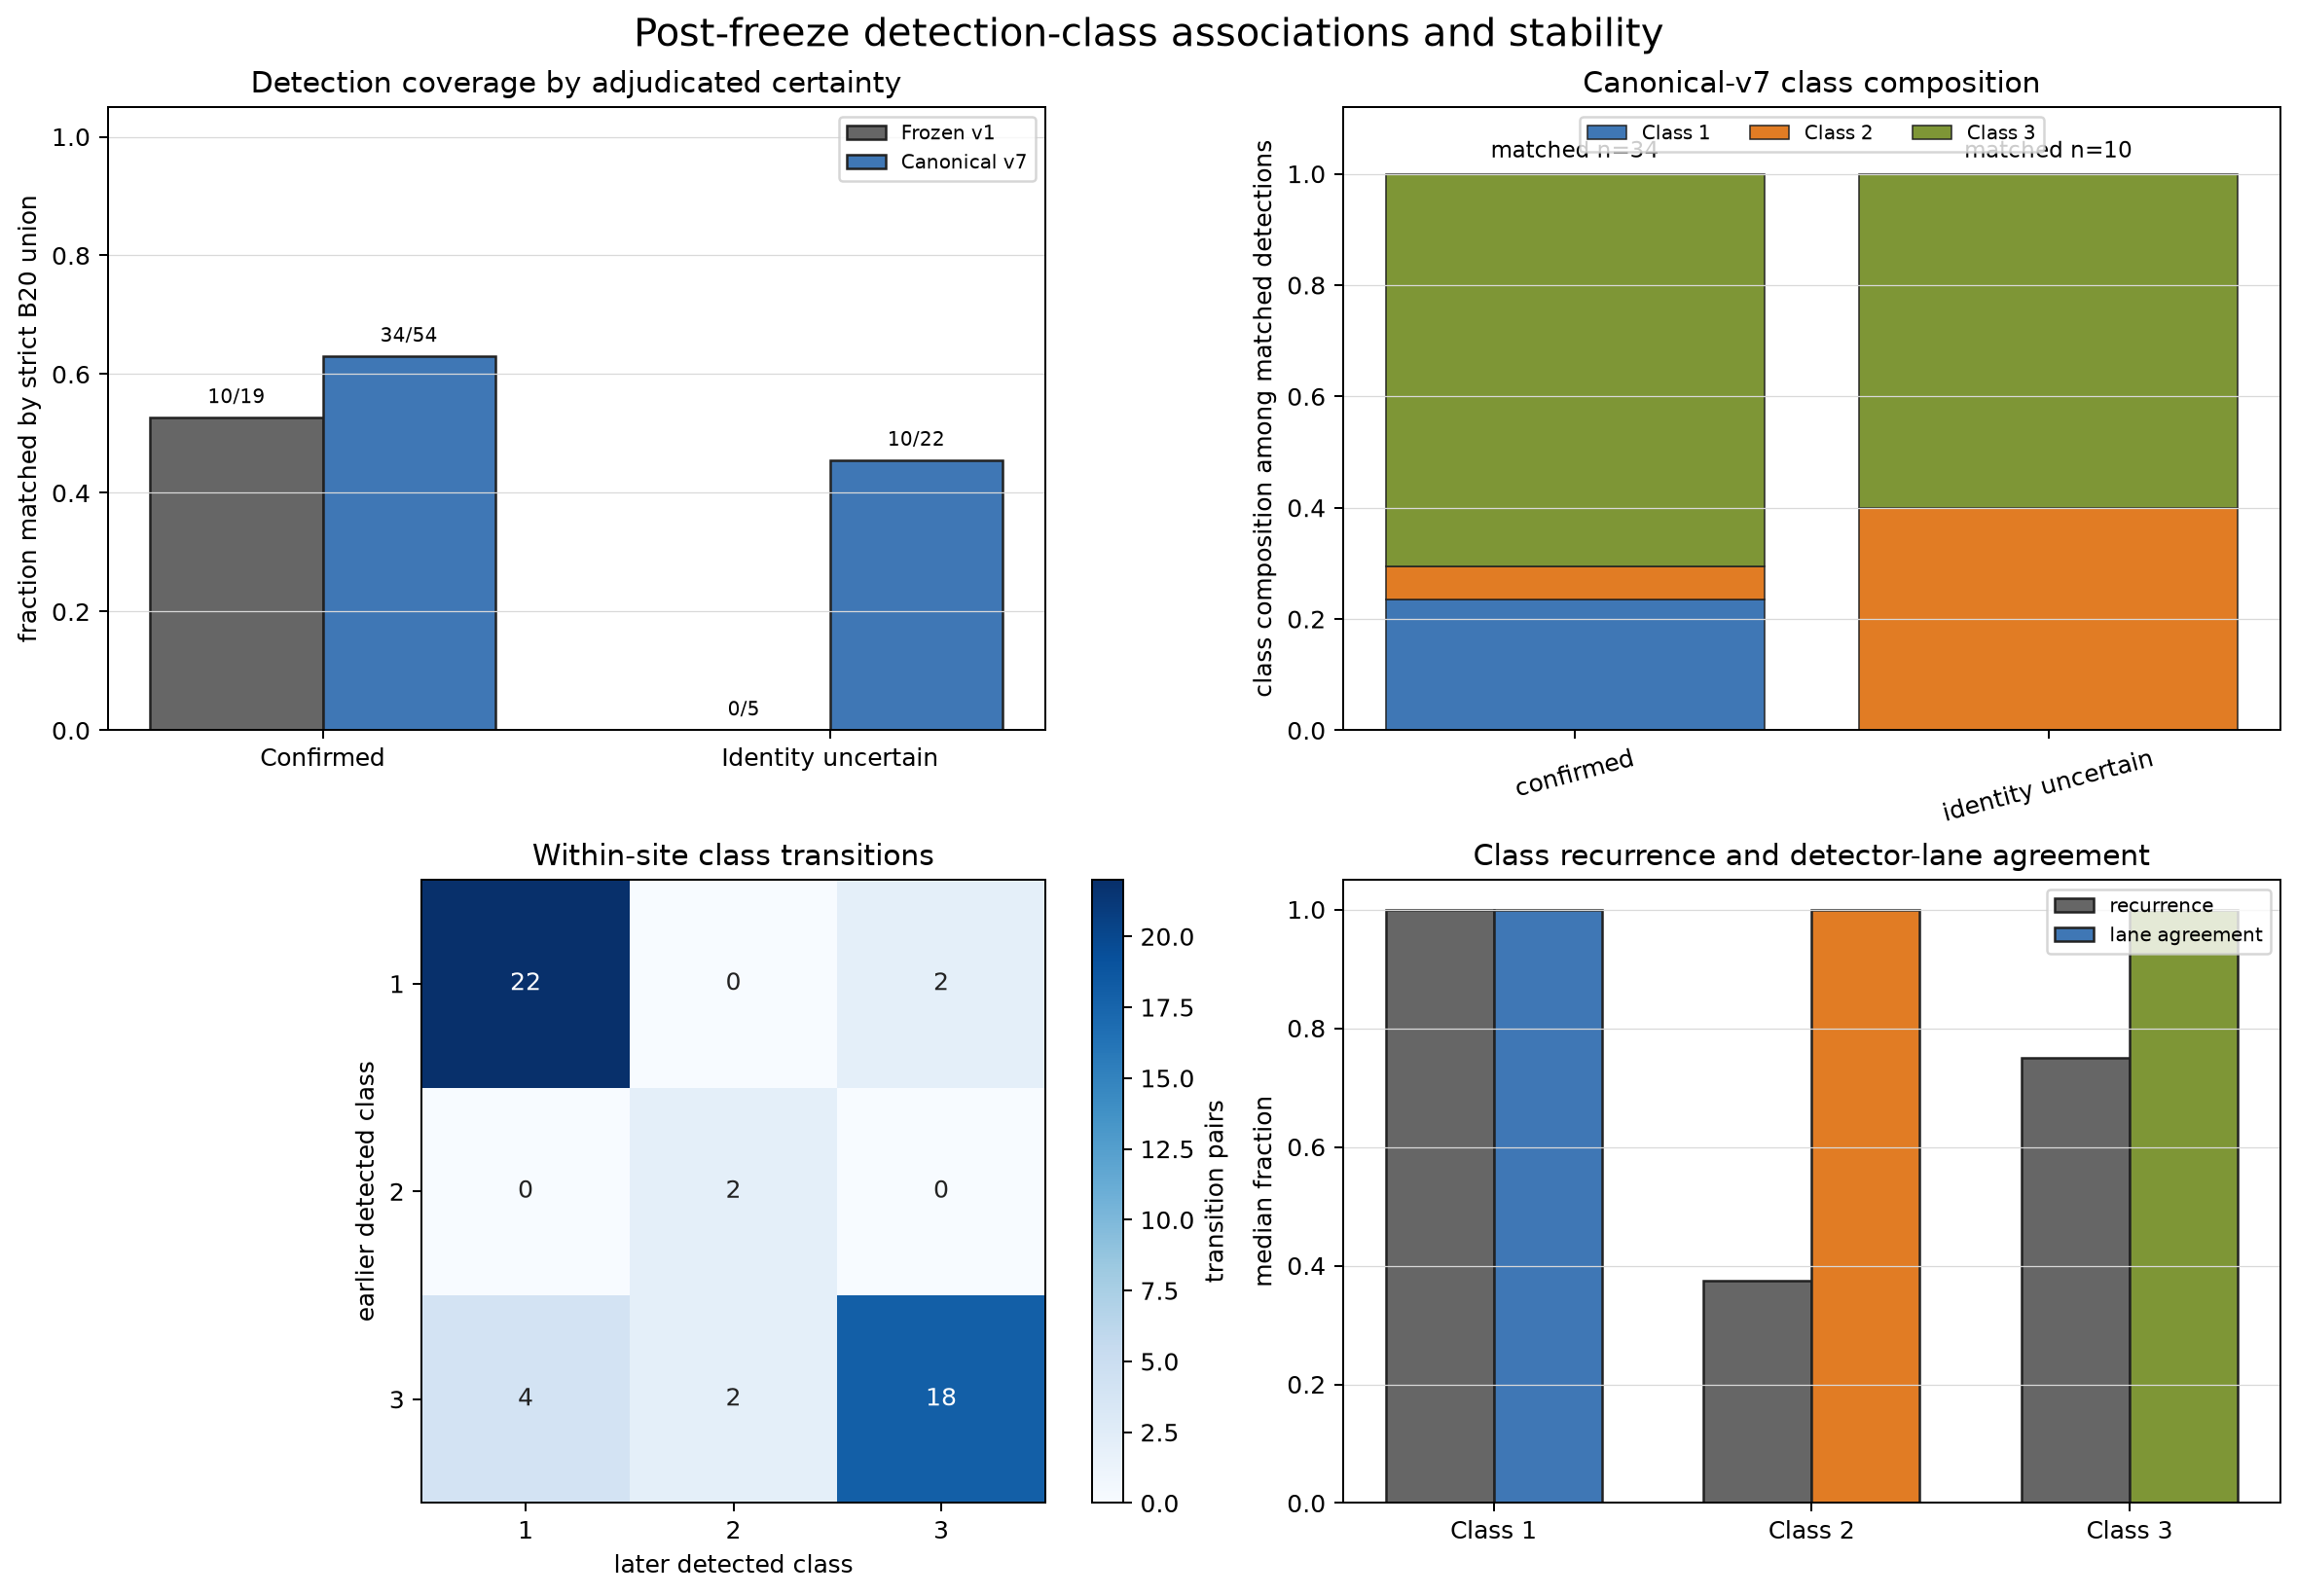
\includegraphics[width=0.98\linewidth]{figures/final/detection_class_extensions.png}
  \caption{Post-freeze class extensions. Detection coverage is reported against adjudicated certainty for frozen v1 and candidate-assisted canonical v7; class composition is shown only where both confirmed and identity-uncertain matched observations are available. The transition matrix follows repeated detection sites across ordered bursts. All associations are descriptive and do not redefine the frozen classes.}
  \label{fig:detection-class-extensions}
\end{figure}

Further post-freeze profiling separated reviewer uncertainty from clustering ambiguity. We defined a relative centroid margin from the nearest and second-nearest frozen class centers; this is a geometric separation measure, not a calibrated probability. Median margins were 0.511, 0.440, and 0.474 for Classes 1--3. Confirmed and identity-uncertain canonical-v7 matches had similar margins (0.473 versus 0.511; Mann--Whitney $p=0.790$). Thus uncertain identity was not explained by detections simply lying near a class boundary.

Reviewer morphology provided a more direct association. Among 45 matched adjudicated canonical-v7 observations, localized-boundary morphology contributed 8, 3, and 27 observations to Classes 1--3, whereas ambiguous or non-neuronal boundary morphology contributed 0, 4, and 3 ($V=0.503$). Challenging or structured contexts contributed 0, 5, and 5 observations, isolated contexts 8, 2, and 20, and overlapping contexts 0, 0, and 5 ($V=0.411$). These candidate-assisted associations reinforce the interpretation of Class 1 as spatially localized and Class 2 as a broad or difficult measurement regime, but they are not independent class validation.

Spatial effects were evaluated at the 36-site consolidated grain to avoid counting recurrent sites repeatedly. Relative to the provisional $x=286$ field boundary, the left/right site counts were 1/9 for Class 1, 2/4 for Class 2, and 0/20 for Class 3. The post hoc site-label permutation value was $p=0.041$ ($V=0.433$). Because only three sites lay left of the boundary and the boundary remains provisional, this result motivates acquisition-field stratification rather than an anatomical class claim. Conversely, burst composition showed little evidence of drift ($V=0.178$, permutation $p=0.503$), consistent with the classes recurring across all four events.

Canonical-v7 matching produced 24 identity trajectories, eight with detections in at least two bursts. The median dominant-class fraction among these multi-burst identities was 1.0, while specific identities such as ROI~014 and ROI-new-002 changed class in one burst. These cases provide a bounded review queue for distinguishing true measurement-regime changes from registration, overlap, or event-amplitude effects.

\subsection{Spatial ICA is localized at labeled coordinates but not temporally persistent}
\label{sec:spatial-ica-results}

Relative to matched translated controls, spatial-ICA event maps had greater center--annulus contrast (mean site-blocked difference \SpatialICAContrastDelta{}, $q=\SpatialICAContrastQ{}$), smaller effective radius (\SpatialICARadiusDelta{} pixels, $q=\SpatialICARadiusQ{}$), and smaller peak offset (\SpatialICAPeakOffsetDelta{} pixels, $q=\SpatialICAPeakOffsetQ{}$). Boundary sharpness was also greater after correction. Compactness and temporal persistence were not supported for spatial ICA. Raw maps showed the same directional localization pattern, with the exception that Raw compactness also differed. These comparisons establish representation-internal localization at protected coordinates, not neuronal identity and not precision against biological negatives.

\begin{figure}[!htbp]
  \centering
  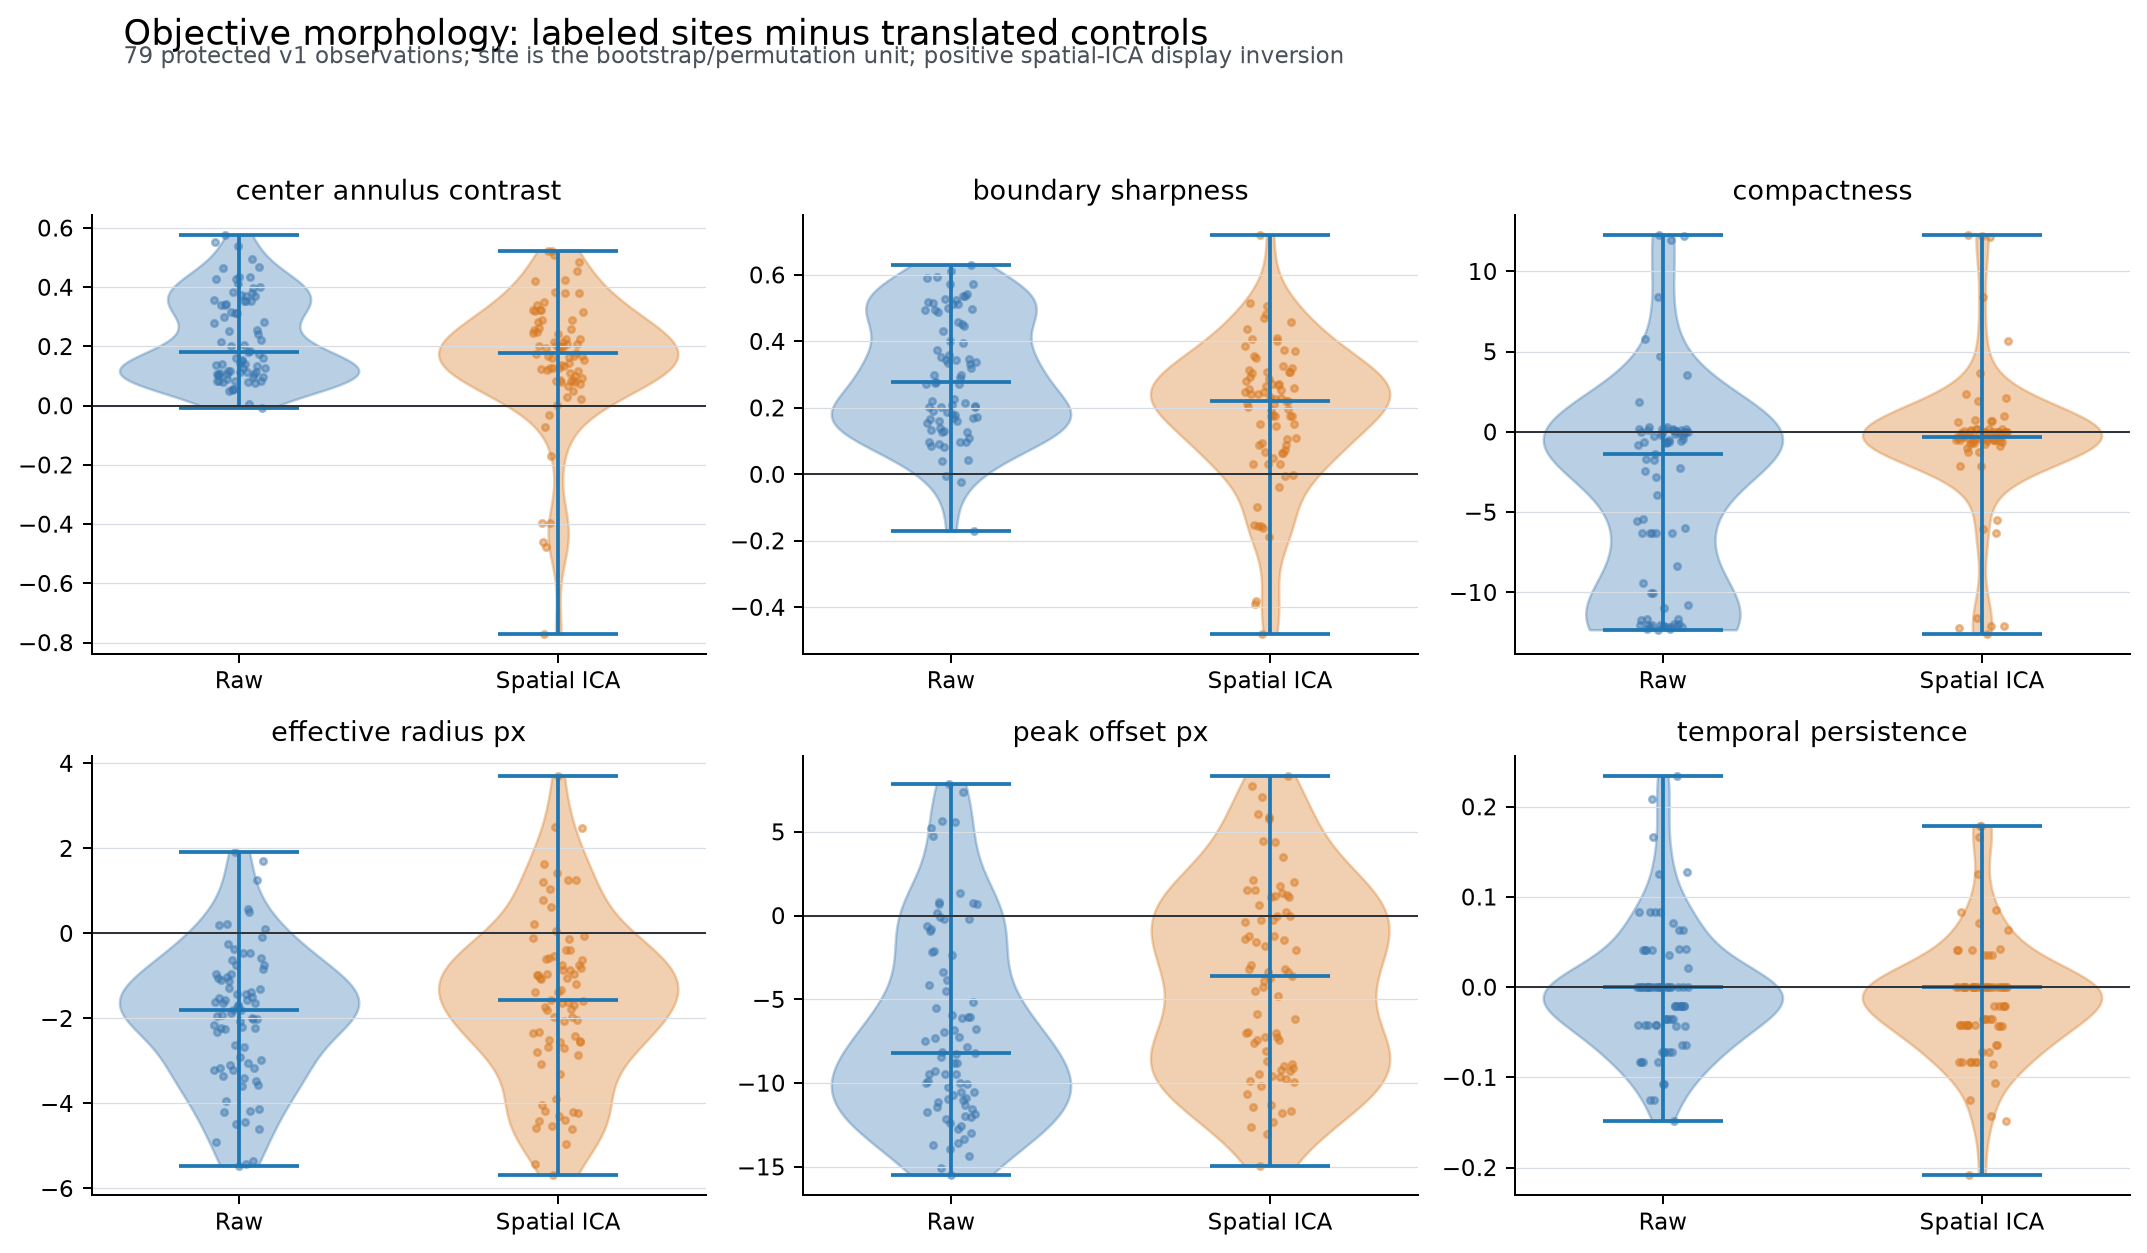
\includegraphics[width=0.98\linewidth]{figures/final/spatial_ica_objective_morphology.png}
  \caption{Objective morphology at protected-v1 coordinates and deterministic translated controls. Paired site-level effects show that Raw and spatial-ICA event maps are more centered and spatially concentrated at labeled locations. Translated locations are unlabeled controls, not verified negatives; units remain representation-specific.}
  \label{fig:spatial-ica-morphology}
\end{figure}

\subsection{Unstable ICA filters yield a highly stable reconstructed representation}

All eight spatial-ICA refits converged, but the filter-level interpretation gates failed. Across nonreference seeds, mean subspace cosine similarity ranged from 0.866 to 0.881 and median aligned individual-filter correlation ranged from 0.639 to 0.710. Leave-one-burst-window-out values ranged from 0.895 to 0.918 and 0.606 to 0.784, respectively. Individual spatial filters therefore cannot be assigned anatomical names or treated as reproducible neuronal components.

The reconstructed output was substantially more stable. Across seed and held-burst variants, the minimum pixel correlation was \SpatialICAMinPixelCorrelation{}, the minimum median event-map correlation was \SpatialICAMinEventMapCorrelation{}, and the minimum median morphology rank correlation was \SpatialICAMinMorphologySpearman{}. Median peak error was zero frames for every variant. Relative to reference known-positive recall of \SpatialICAReferenceRecall{}, seed changes ranged from $-0.0125$ to $+0.0109$, while every held-burst recall change was exactly zero. All prespecified reconstruction gates passed. Thus the defensible object is the reconstructed spatial-ICA representation, not any individual basis filter.

\begin{figure}[!htbp]
  \centering
  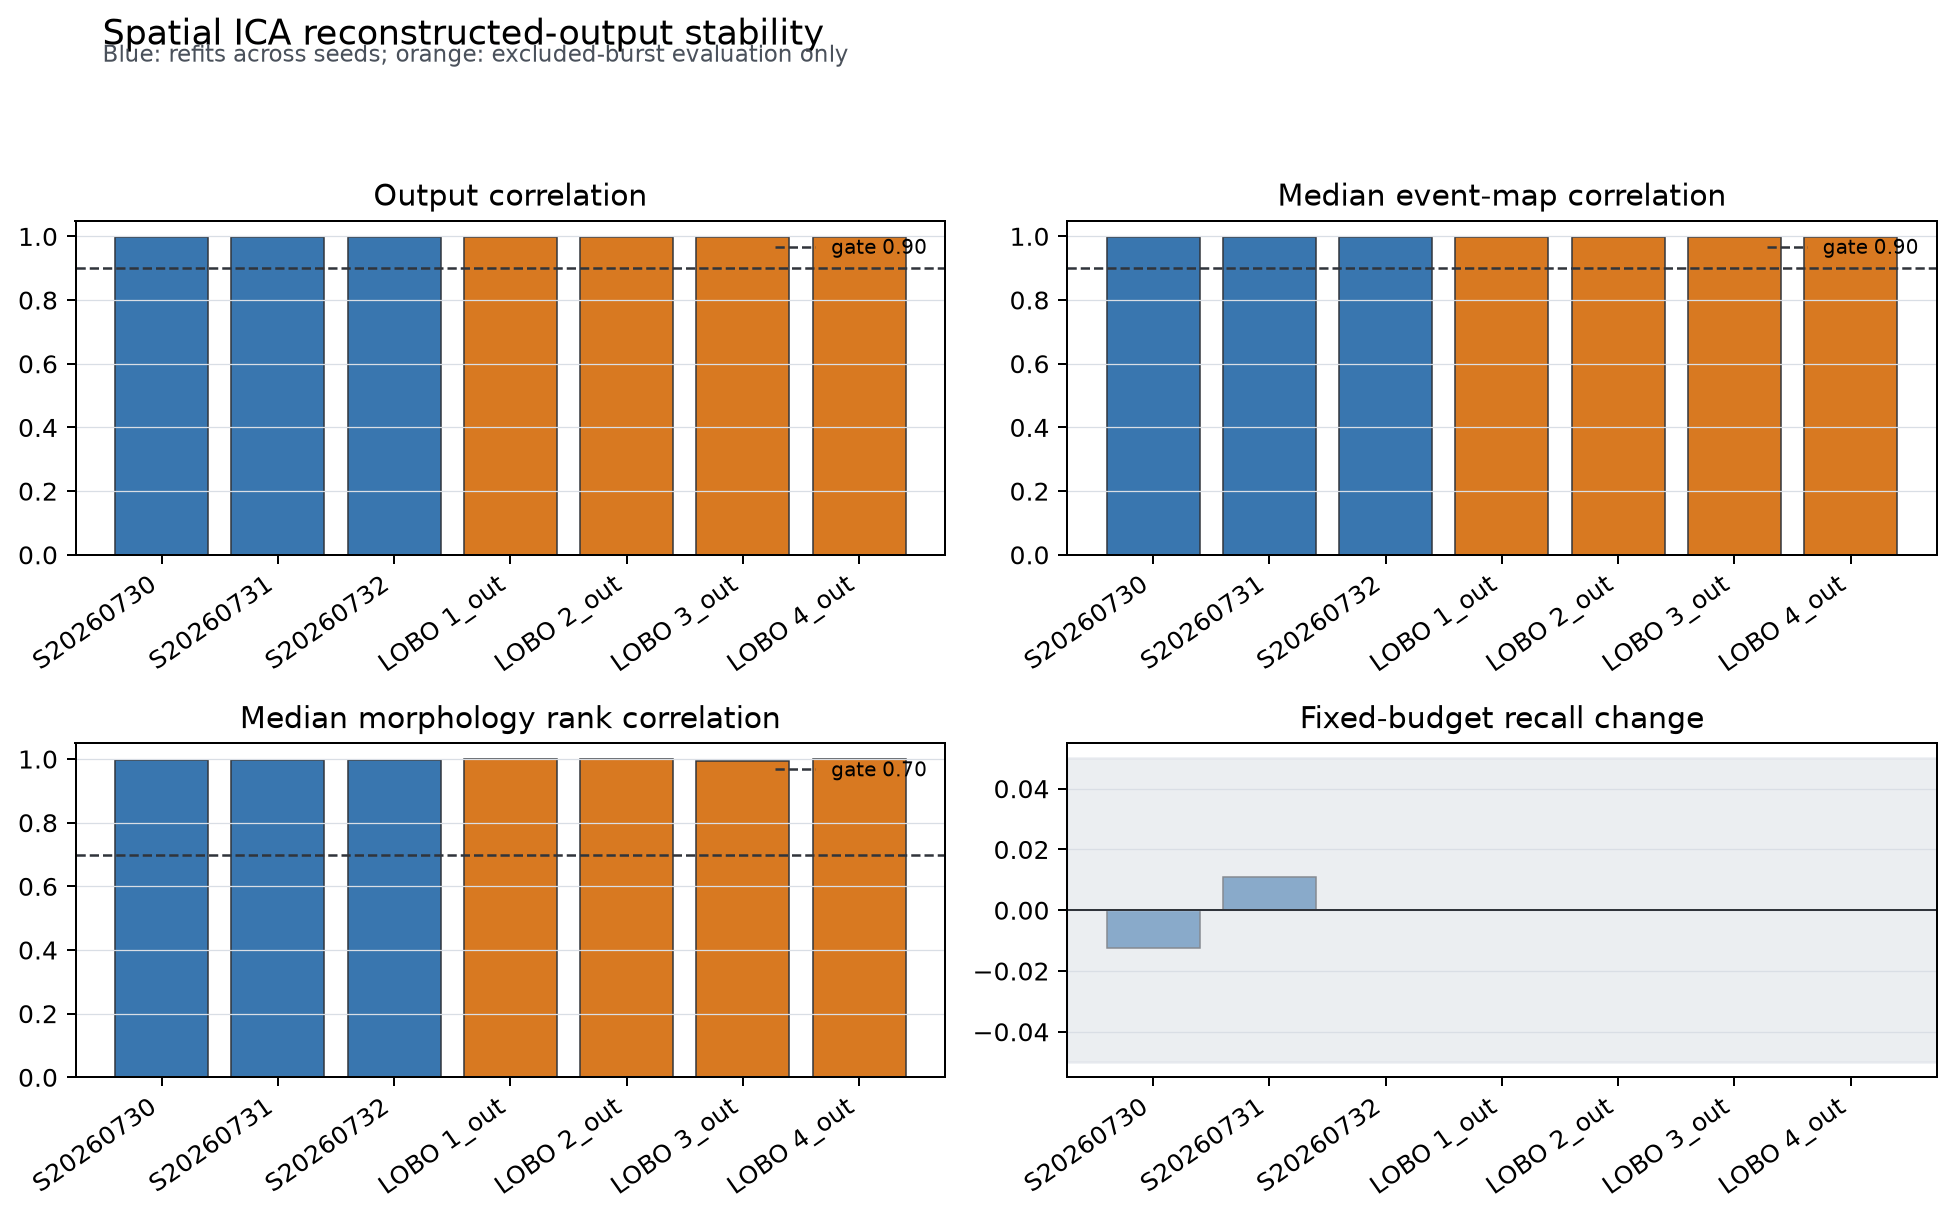
\includegraphics[width=0.98\linewidth]{figures/final/spatial_ica_reconstruction_stability.png}
  \caption{Spatial-ICA reconstructed-output stability across random seeds and leave-one-burst-window-out refits. Correlations, morphology-rank agreement, peak timing, and fixed-budget known-positive recall remained within the prespecified gates.}
  \label{fig:spatial-ica-reconstruction-stability}
\end{figure}

\subsection{Class and certainty alignment remain suggestive, not validated}

The 53 protected-v1 one-to-one matches collapsed to 17 immutable sites with dominant-class counts 7, 1, and 9. Only one Class~2 site made a protected three-class comparison inadmissible. Across 14 protected class--morphology tests, no spatial-ICA metric approached corrected significance; the two smallest corrected values ($q=0.0588$) were Raw contrast and Raw boundary sharpness, metrics partially overlapping the spatial-specificity feature used to fit the classes.

In candidate-assisted canonical v7, the 24 identities had dominant-class counts 3, 5, and 16. The strongest spatial-ICA association was boundary sharpness ($\epsilon^2=\SpatialICAVsevenBoundaryEpsilon{}$, nominal $p=0.00485$), but it did not survive the 14-test correction ($q=\SpatialICAVsevenBoundaryQ{}$). Its class medians were $-0.022$, $0.018$, and $0.263$, providing a concrete hypothesis for independent data rather than a confirmed class distinction.

Confirmed identities had dominant-class counts 3, 2, and 10, compared with 0, 3, and 6 for identity-uncertain identities. At the canonical-identity grain, the association was not supported (Cramer's $V=\CertaintyDominantClassCramersV{}$, permutation $p=\CertaintyDominantClassPermutationP{}$). After adjustment for class and burst, none of 14 Raw or spatial-ICA morphology metrics distinguished the 15 confirmed from nine uncertain identities after multiplicity correction, and every bootstrap interval included zero. The data therefore do not establish that the frozen classes or objective ICA morphology encode reviewer certainty.

\begin{figure}[!htbp]
  \centering
  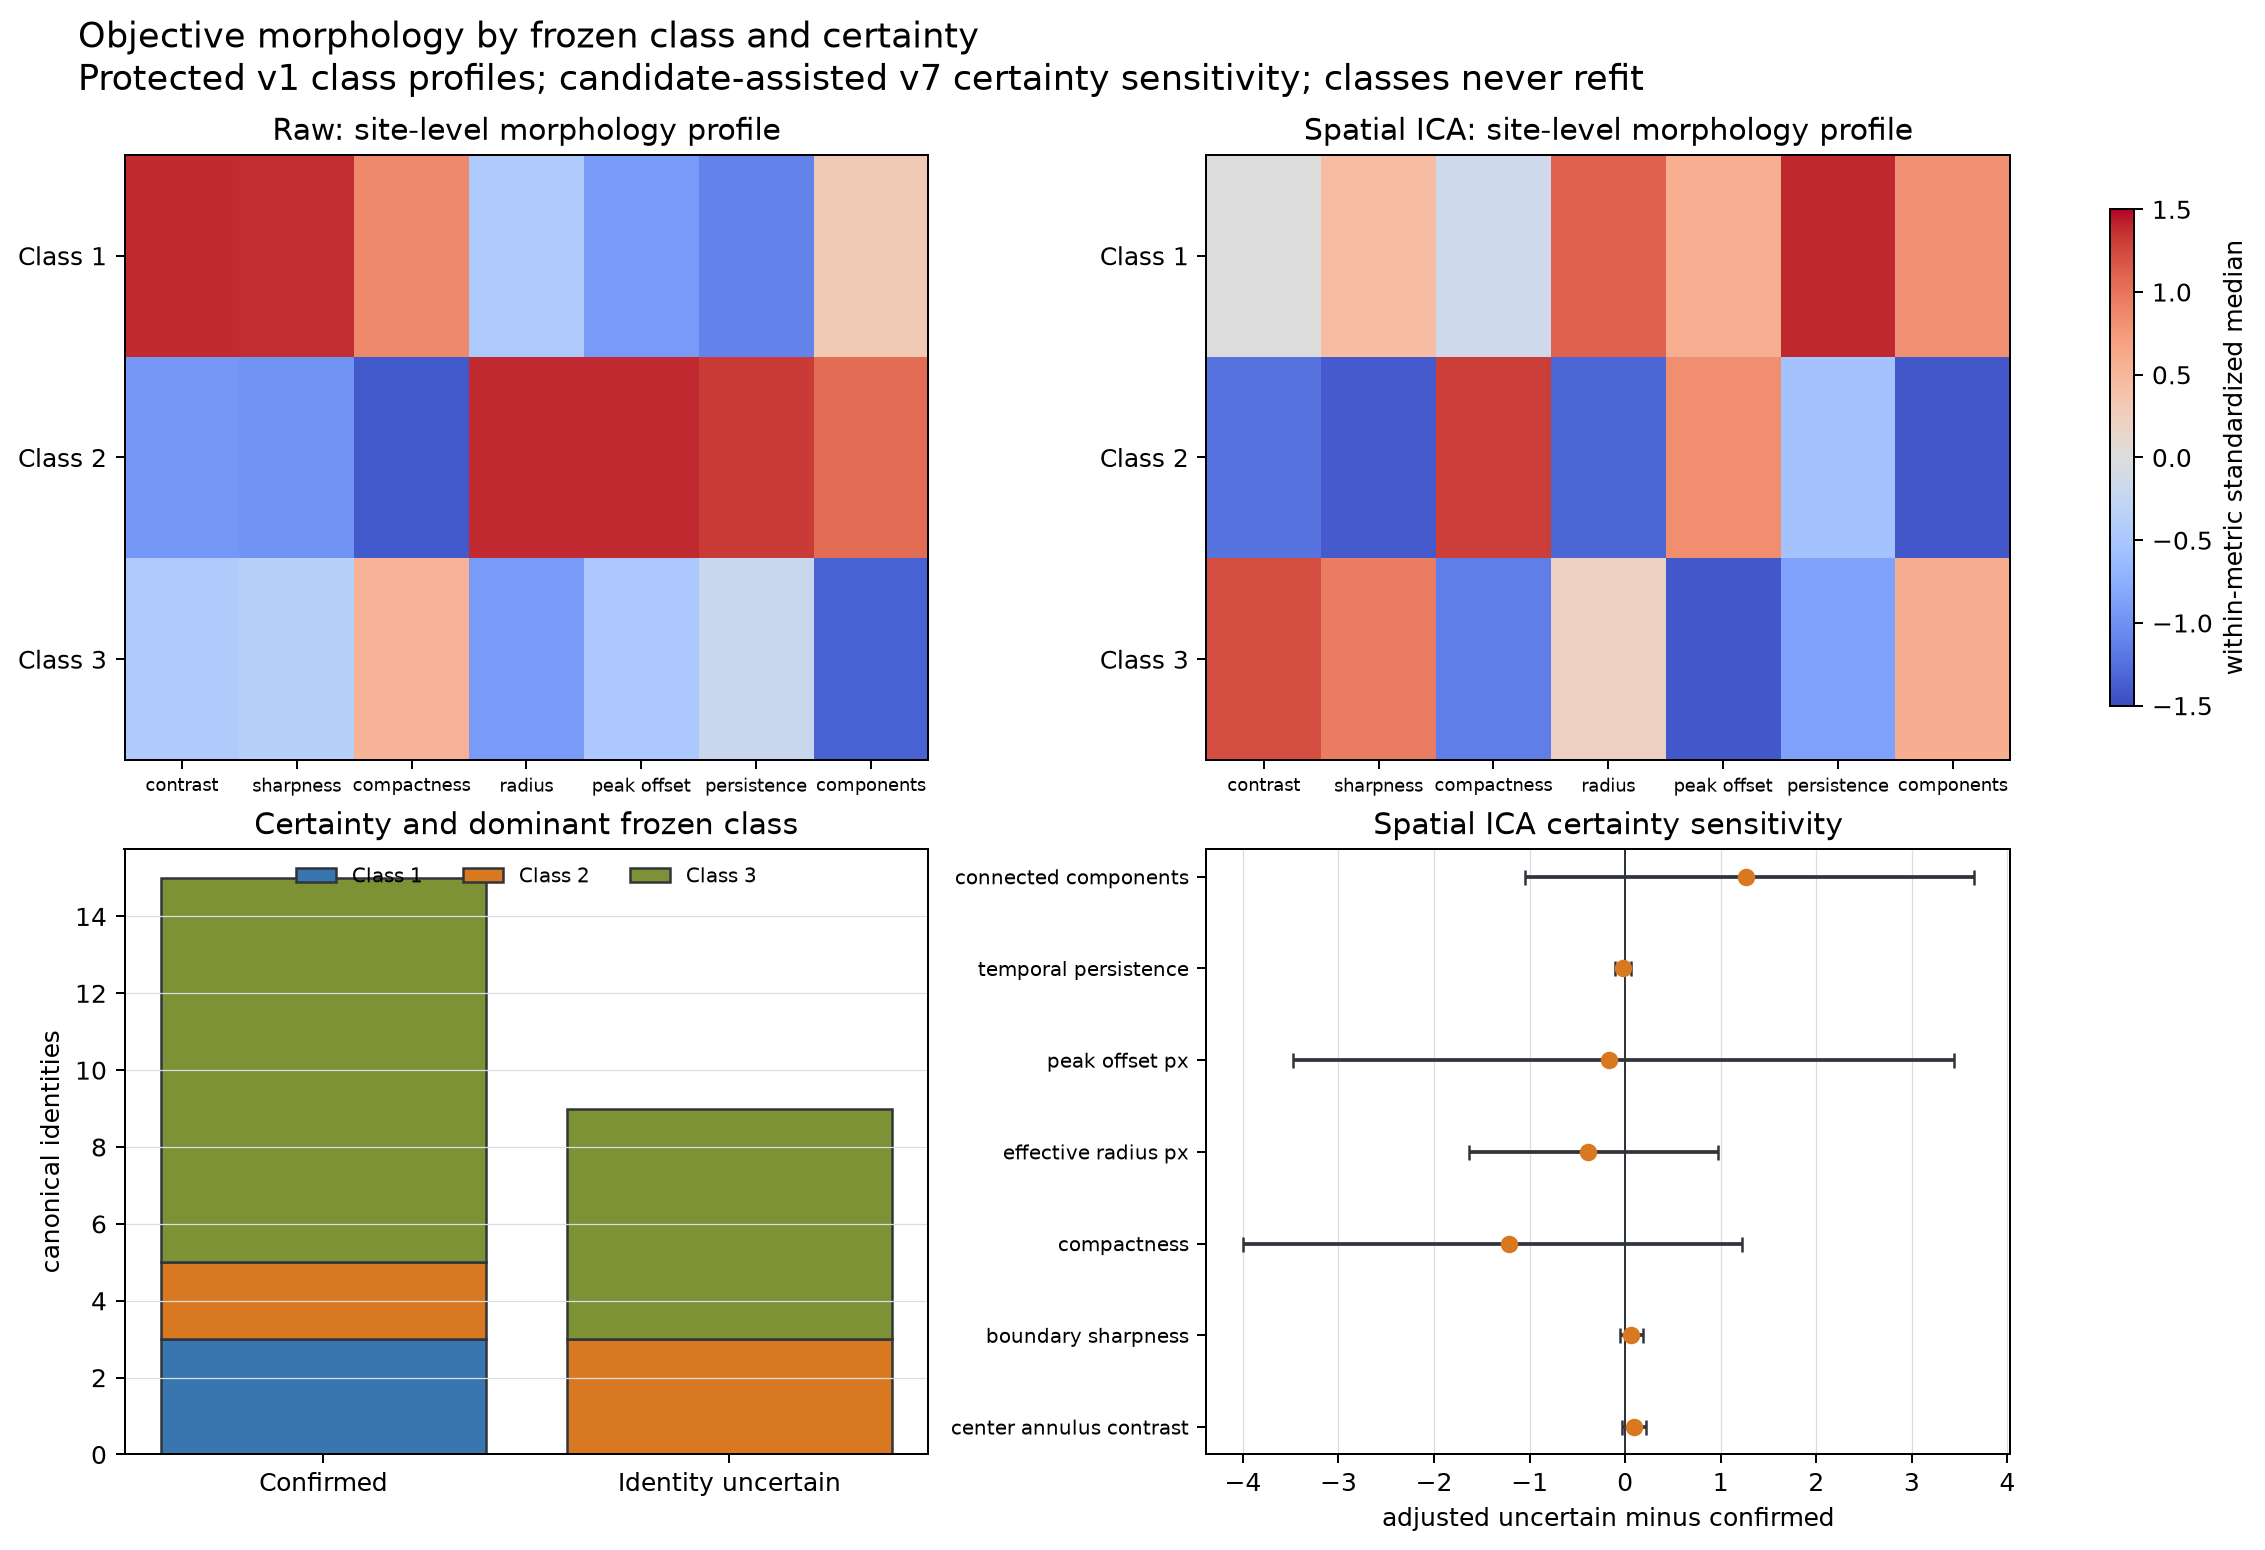
\includegraphics[width=0.98\linewidth]{figures/final/spatial_ica_class_certainty.png}
  \caption{Protected-v1 and canonical-v7 class/certainty alignment with objective morphology. Protected three-class inference is blocked by a single Class~2 site; canonical-v7 certainty comparisons are candidate-assisted and aggregated at canonical identity.}
  \label{fig:spatial-ica-class-certainty}
\end{figure}

\begin{figure}[!htbp]
  \centering
  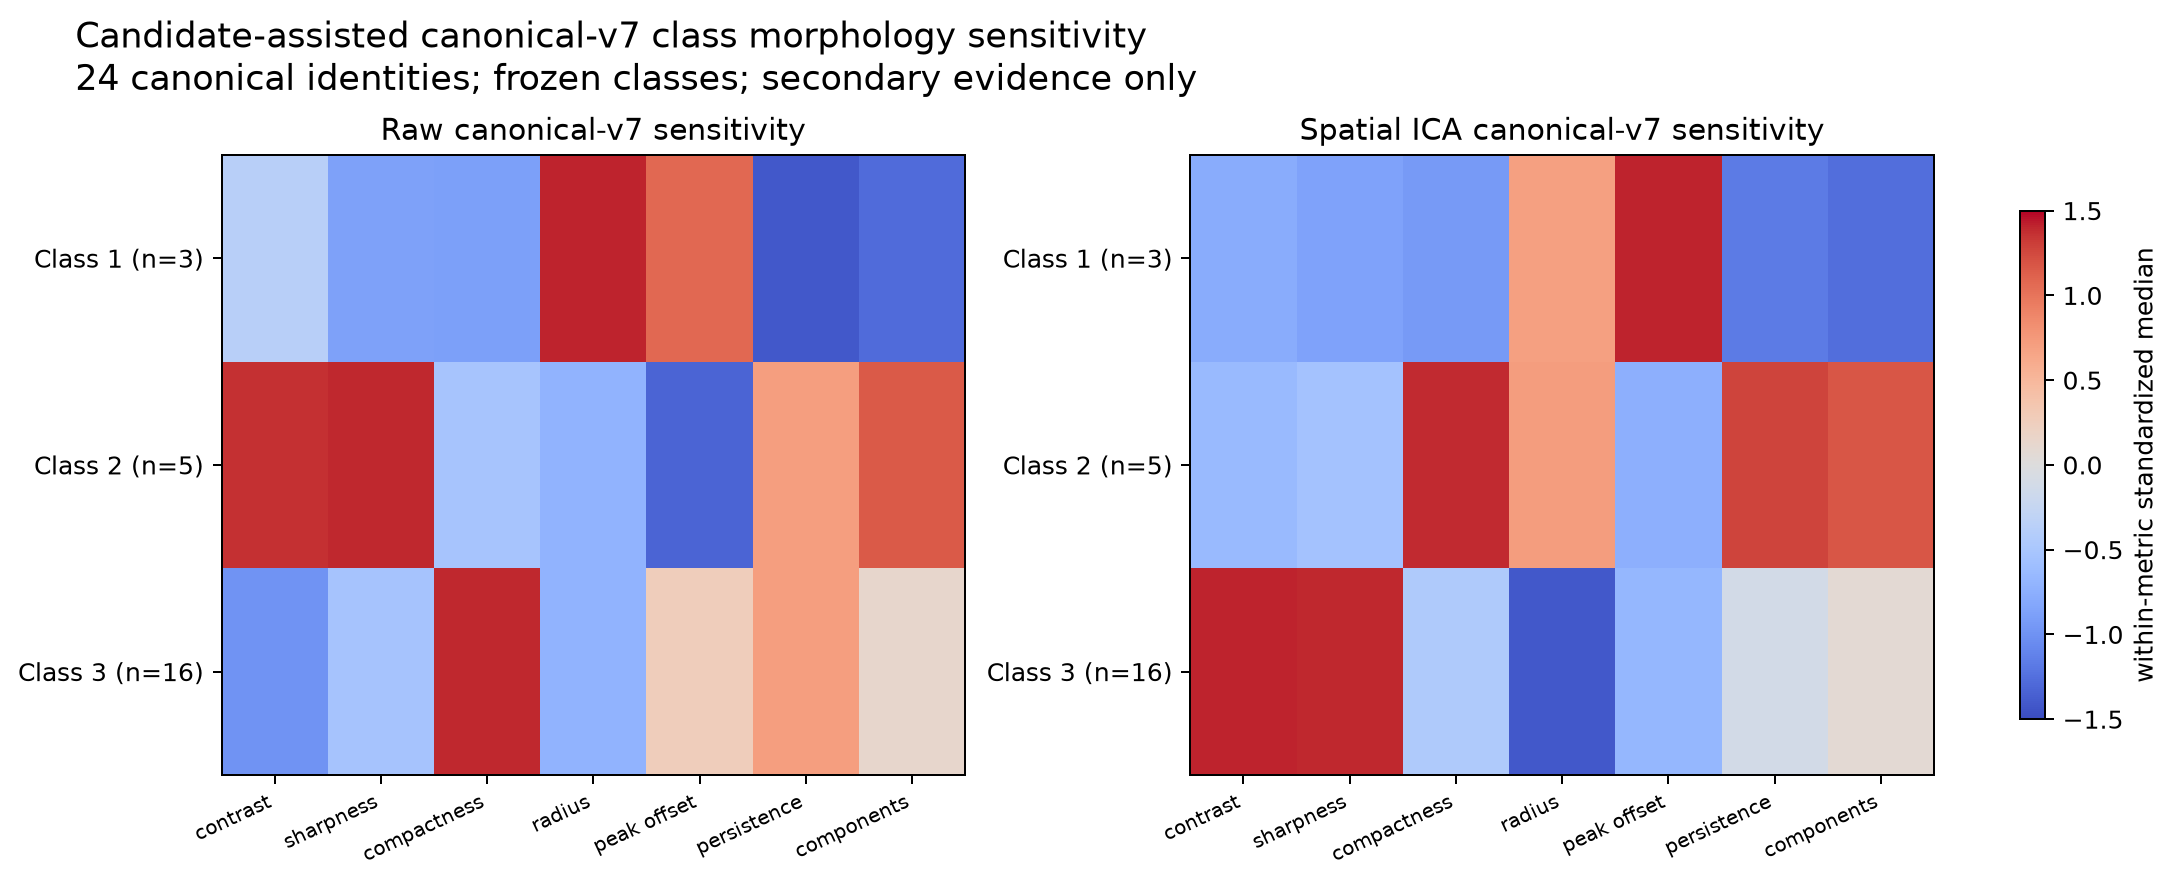
\includegraphics[width=0.98\linewidth]{figures/final/spatial_ica_canonical_v7_sensitivity.png}
  \caption{Candidate-assisted canonical-v7 sensitivity of objective morphology across dominant frozen classes. Spatial-ICA boundary sharpness is the strongest descriptive separation but does not survive family-wise false-discovery-rate control.}
  \label{fig:spatial-ica-v7-sensitivity}
\end{figure}

\subsection{Prespecified confirmatory hypotheses}

The protected rerun follows the hypothesis hierarchy in \Cref{tab:hypotheses}. Functional and tensor analyses are promoted only if trace completeness, held-out reconstruction, and component-stability gates pass. A null or heterogeneous result remains scientifically reportable because it defines the boundary between shared burst detection and neuron-specific identification.

\begingroup
\footnotesize
\setlength{\tabcolsep}{3pt}
\setlength{\LTpre}{0.4\baselineskip}
\setlength{\LTpost}{0.4\baselineskip}
\begin{longtable}{p{0.055\textwidth} >{\raggedright\arraybackslash}p{0.34\textwidth} >{\raggedright\arraybackslash}p{0.19\textwidth} >{\raggedright\arraybackslash}p{0.32\textwidth}}
\caption{Prespecified hypothesis hierarchy for the protected analysis.}\label{tab:hypotheses}\\
\toprule
ID & Hypothesis & Current status & Confirmatory decision rule \\
\midrule
\endfirsthead
\multicolumn{4}{l}{\small\itshape Table \thetable\ continued from previous page}\\
\toprule
ID & Hypothesis & Current status & Confirmatory decision rule \\
\midrule
\endhead
\midrule
\multicolumn{4}{r}{\small\itshape Continued on next page}\\
\endfoot
\bottomrule
\endlastfoot
H1 & Annotated events differ from matched ordinary times. & Supported provisionally. & Site/burst-aware block-shift effect and interval exclude the null region. \\
H2 & Event activity is spatially concentrated at the labeled site. & Partial amplitude evidence. & ROI contrasts outperform matched spatial controls; equivalence assessed only with frozen margins. \\
H3 & Sites or neurons possess stable activation gain/observability. & Strong exploratory motivation. & Cross-burst rank stability and site variance component pass preregistered reliability gates. \\
H4 & Neurons possess reproducible neuron-specific temporal waveforms. & Not established. & Functional site component improves held-out reconstruction and exceeds spatial controls. \\
H5 & Measurement phenotype explains known-positive recovery failures. & Suggestive. & Prespecified covariates improve held-out recovery model with stable coefficient direction. \\
H6 & Two-frame ICA adds information beyond temporal difference. & Provisionally rejected. & Promote only if repaired rerun breaks the analytic equivalence and adds utility/fidelity. \\
H7 & Compact spatial/contextual statistics add recovery information. & Supported provisionally. & Frozen same-proposal and proposal-union comparisons improve known-positive recall without disproportionate burden. \\
H8 & Directed or network interactions are identifiable. & Not established. & Exploratory only; no causal promotion from this recording. \\
\end{longtable}
\endgroup

